The di-Higgs analysis is divided in two channels depending on the di-$\tau$ decay mode: \lephad and \hadhad. Triggers and event selection requirements applied in the two channels are described in the following.

\subsection{Trigger}
\label{subsec:trigger}
\subsubsection{\lephad trigger selection}
\label{sec:lephadtrigger}
In the \lephad channel, events are selected using single lepton triggers (SLT) and lepton tau triggers (LTT). 

The priority is given to SLT events if a lepton ($e$ or $\mu$) fulfils the offline lepton \pT requirements.
Single muon triggers (SMT) require an event with a muon with \pT > 21 or > 27~\GeV, whereas single electron triggers (SET)
require an event with an electron with \pT > 25 or > 27~\GeV, depending on the data-taking period.
The SLT triggers used are listed in Table \ref{tab:SLTtriggers_lephad}. 

If the event fails the SLT, then the LTT is checked. The LTT requires either an electron with \pT >18~\GeV~or a
muon with \pT > 15~\GeV. The \pT threshold for \tauhad is 30 \GeV. The complete list of LTT triggers, along with the trigger-dependent offline \pT thresholds, are
shown in Table \ref{tab:LTTtriggers_lephad}, where the abbreviations for the trigger names are used.
The full name of these triggers can be found in Table \ref{tab:LTT_trigger_names} of Appendix \ref{sec:appendix_LTT_trigger_names}.

Both for muon and electron channels, \verb|*_tau25(_EF)| triggers require one additional jet with 25 \GeV\ at L1. 
That necessitates to require one jet with offline \pT > 80 \GeV~in the analysis.

Triggers with L1 seeds \verb|*_4J12| and \verb|*_3J12|, also require additional jets at L1,
which necessitates to require two jets with offline \pT > 45 \GeV~in the analysis.

There is no jet requirement at L1 for \verb|mu14_tau35(_EF)|. 

When an OR of multiple triggers is used in the electron channel (ETT), \verb|*_4J12| trigger is prioritized due to lower jet \pT thresholds. 
This means that, other triggers are checked if and only if  \verb|*_4J12| doesn't fire. The offline selection is adjusted accordingly, as shown in Table \ref{tab:LTTtriggers_lephad}.

For 2017 and 2018 data-taking periods, different muon tau triggers (MTT)
are used for two different regions defined by 30 \GeV~< $\pT^{\tau} \leq$ 40 \GeV~ and $\pT^{\tau}$ > 40 \GeV. 

For 2018 data-taking period, starting from Period K, the recommendation is to use a logical OR between 
BDT and RNN triggers.

Studies on the lepton tau trigger selection can be found in Appendix\ref{subsec:appendix_selection_trigger}.

\begin{table}
 % \centering
  \scriptsize
  \hspace{-43pt}
  \begin{tabular}{llclcc}
  %  \toprule
    %Trigger & Period \\
    \midrule
    \multicolumn{6}{c}{\textbf{Single Lepton Triggers (SLT)}} \\
    \midrule
    \textbf{Period} & \textbf{Single Electron Triggers (SET)} &  \textbf{$e$ \pT [GeV]}  & \textbf{Single Muon Triggers (SMT)} & \textbf{$\mu$ \pT [GeV]} &  \textbf{Leading (Sub-leading) jet \pT [GeV]}  \\
    \midrule 
    \multirow{3}{*}{2015} & HLT\_e24\_lhmedium\_L1EM20VH() & \multirow{3}{*}{25}&HLT\_mu20\_iloose\_L1MU15 & \multirow{3}{*}{21} & \multirow{3}{*}{45 (20)} \\
    & HLT\_e60\_lhmedium & & HLT\_mu50 & & \\
    & HLT\_e120\_lhloose & & & &\\
    \midrule
    \multirow{3}{*}{2016 \& 2017 \& 2018} & HLT\_e26\_lhtight\_nod0\_ivarloose &\multirow{3}{*}{27} & HLT\_mu26\_ivarmedium & \multirow{3}{*}{27} & \multirow{3}{*}{45 (20)} \\
    & HLT\_e60\_lhmedium\_nod0 & & HLT\_mu50 & &\\
    & HLT\_e140\_lhloose\_nod0 &  &	& & \\
 \bottomrule
  \end{tabular}
 \caption{SLT triggers used in the \lephad channel, along with the trigger-dependent offline \pT thresholds, for each year/period are shown.}
  \label{tab:SLTtriggers_lephad}
\end{table}


%\begin{table}[h]
%  \centering
% \scriptsize
%  \begin{tabular}{lll}
%  %  \toprule
%    %Trigger & Period \\
%    \midrule
%    \multicolumn{2}{c}{Lepton Tau Triggers (LTT)} \\
%    \midrule
%   Electron Tau Triggers (ETT)  &  Period   \\
%    \midrule
%      HLT\_e17\_lhmedium\_nod0\_tau25\_medium1\_tracktwo  & 15-16 A \\	
%      HLT\_e17\_lhmedium\_nod0\_ivarloose\_tau25\_medium1\_tracktwo  & 16 B-\\
%      HLT\_e17\_lhmedium\_nod0\_ivarloose\_tau25\_medium1\_tracktwo &  17 \\
%      HLT\_e17\_lhmedium\_nod0\_ivarloose\_tau25\_medium1\_tracktwo\_L1EM15VHI\_2TAU12IM\_4J12 & 17  \\
%      HLT\_e17\_lhmedium\_nod0\_ivarloose\_tau25\_medium1\_tracktwoEF & 18 B-\\
%      HLT\_e17\_lhmedium\_nod0\_ivarloose\_tau25\_medium1\_tracktwoEF\_L1EM15VHI\_2TAU12IM\_4J12& 18 B-   \\
%      HLT\_e17\_lhmedium\_nod0\_ivarloose\_tau25\_mediumRNN\_tracktwoMVA & 18 K-  \\
%      HLT\_e17\_lhmedium\_nod0\_ivarloose\_tau25\_mediumRNN\_tracktwoMVA\_L1EM15VHI\_2TAU12IM\_4J12 & 18 K- \\
%   \midrule
%    Muon Tau Triggers (MTT) & Period \\
%     \midrule
%      HLT\_mu14\_tau25\_medium1\_tracktwo & 15-16 A \\		
%      HLT\_mu14\_ivarloose\_tau25\_medium1\_tracktwo & 16 B- \\
%      HLT\_mu14\_ivarloose\_tau35\_medium1\_tracktwo  & 17~~~~~~($\mathrm{For}~\pt^{\tau} > 40$ \GeV) \\
%      HLT\_mu14\_ivarloose\_tau25\_medium1\_tracktwo\_L1MU10\_TAU12IM\_3J12 & 17~~~~~~($\mathrm{For}~\pt^{\tau} < 40$ \GeV)  \\
%      HLT\_mu14\_ivarloose\_tau35\_medium1\_tracktwoEF & 18 B- ($\mathrm{For}~\pt^{\tau} > 40$ \GeV) \\
%      HLT\_mu14\_ivarloose\_tau25\_medium1\_tracktwoEF\_L1MU10\_TAU12IM\_3J12 & 18 B- ($\mathrm{For}~\pt^{\tau} < 40$ \GeV) \\
%      HLT\_mu14\_ivarloose\_tau35\_mediumRNN\_tracktwoMVA & 18 K- ($\mathrm{For}~\pt^{\tau} > 40$ \GeV) \\
%      HLT\_mu14\_ivarloose\_tau25\_mediumRNN\_tracktwoMVA\_L1MU10\_TAU12IM\_3J12 & 18 K- ($\mathrm{For}~\pt^{\tau} < 40$ \GeV) \\
%    \bottomrule
%  \end{tabular}
%  \caption{LTT triggers used for data taking in the \lephad channel.}
%  \label{tab:LTTtriggers_lephad}
%\end{table}

\begin{table}
  \centering
 \scriptsize
  \begin{tabular}{llccc}
    \toprule
    %Trigger & Period \\
    \multicolumn{5}{c}{\textbf{LEPTON TAU TRIGGERS (LTT)}} \\
    \toprule
    \toprule
     \textbf{Period} & \textbf{Electron Tau Triggers (ETT)} & \textbf{$e$ \pT [GeV]} & \textbf{$\tau_{\mathrm{had}}$ \pT [GeV]} & \textbf{Leading (Sub-leading) jet \pT [GeV]}  \\
    \toprule
      15-16 A  & e17\_tau25 & 18 & 30 & 80 (20) \\	
     \midrule
      16 B-      & e17\_ivarloose\_tau25 & 18 & 30 & 80 (20)\\
      \midrule
      \multirow{2}{*}{17}  & e17\_ivarloose\_tau25\_4J12 OR &  \multirow{2}{*}{18} & \multirow{2}{*}{30} & if pass 4J12: 45 (45) \\
                                     & e17\_ivarloose\_tau25 &  & & else: 80 (20)\\
     \midrule
      \multirow{2}{*}{18 B-}  &e17\_ivarloose\_tau25\_EF\_4J12 OR &  \multirow{2}{*}{18} & \multirow{2}{*}{30} & if pass 4J12: 45 (45)\\
                                          & e17\_ivarloose\_tau25\_EF  &  & & else: 80 (20)\\
      \midrule
      \multirow{4}{*}{18 K-} & e17\_ivarloose\_tau25\_EF\_4J12  OR &  \multirow{4}{*}{18} & \multirow{4}{*}{30} & \multirow{2}{*}{if pass 4J12: 45 (45)}\\
      	                   & e17\_ivarloose\_tau25\_RNN\_4J12 OR &  & & \\
                           &  e17\_ivarloose\_tau25\_EF OR &  & &  \multirow{2}{*}{else: 80 (20)}\\
                           & e17\_ivarloose\_tau25\_RNN  & & &\\
   \bottomrule
   \toprule
    \textbf{Period} & \textbf{Muon Tau Triggers (MTT)} & \textbf{$\mu$ \pT [GeV]} & \textbf{$\tau_\mathrm{had}$ \pT [GeV]} & \textbf{Leading (Sub-leading) jet \pT [GeV]} \\
     \toprule
      15-16 A    & mu14\_tau25 &  15 & 30 & 80 (20)\\	
      \midrule	
      16 B-        & mu14\_ivarloose\_tau25 & 15 & 30 & 80 (20)\\
      \midrule
      \multirow{2}{*}{17} & mu14\_ivarloose\_tau25\_3J12  & 15 & (30,40] &45 (45) \\  \cmidrule{2-5}
                      & mu14\_ivarloose\_tau35 &15 & 40 & 45 (20) \\
      \midrule
      \multirow{2}{*}{18 B-}  & mu14\_ivarloose\_tau25\_EF\_3J12 & 15 & (30,40] & 45 (45) \\ \cmidrule{2-5}
                      & mu14\_ivarloose\_tau35\_EF & 15 & 40 & 45 (20) \\
      \midrule
        \multirow{4}{*}{18 K-}  & (mu14\_ivarloose\_tau25\_EF\_3J12 OR & \multirow{2}{*}{15} &  \multirow{2}{*}{(30,40]} & \multirow{2}{*}{45 (45)}\\
                     & mu14\_ivarloose\_tau25\_RNN\_3J12) & & &\\ \cmidrule{2-5}
                     & (mu14\_ivarloose\_tau35\_EF OR &\multirow{2}{*}{15} & \multirow{2}{*}{40}  & \multirow{2}{*}{45 (20)}\\
                     & mu14\_ivarloose\_tau35\_RNN) & & &\\                     
    \bottomrule
  \end{tabular}
  \caption{LTT triggers used in the \lephad channel, along with the trigger-dependent offline \pT thresholds, for each year/period are shown. 
  These triggers are checked when the event fails the SLT triggers. 
  When an OR of multiple triggers is used in the electron channel, 4J12 trigger is prioritized due to lower jet \pT thresholds. 
  This means that, other triggers are checked if and only if 4J12 doesn't fire. The offline selection is adjusted accordingly, as shown in the table.
 For 2017 and 2018 MTT triggers, different muon tau triggers (MTT) are used for two different regions defined by 30 \GeV~< $\pT^{\tau} \leq$ 40 \GeV~ and $\pT^{\tau}$ > 40 \GeV. 
  Abbreviations are used for the trigger names in this table. Table \ref{tab:LTT_trigger_names} of Appendix \ref{sec:appendix_LTT_trigger_names}.}
  \label{tab:LTTtriggers_lephad}
\end{table}

\subsubsection{\hadhad trigger selection}
\label{sec:hadhad_trigger_selection}

In the \tauhad\tauhad channel, events are selected using single (STT) and di-\tauhad
triggers (DTT). The list of triggers used can be found in Table~\ref{tab:triggers_hadhad}.

\begin{table}
  \centering

  \scriptsize

  \begin{tabular}{ll}
    \toprule
    Trigger & Period \\

    \midrule
    \multicolumn{2}{c}{Single \tauhad triggers (STT)} \\
    \midrule

    HLT\_tau80\_medium1\_tracktwo\_L1TAU60 & 15 -- 16 A \\
    HLT\_tau125\_medium1\_tracktwo & 16 B -- 16 D3 \\
    HLT\_tau160\_medium1\_tracktwo & 16 D4 -- 17 B4 \\
    HLT\_tau160\_medium1\_tracktwo\_L1TAU100 & 17 B5 -- 17 end \\
    HLT\_tau160\_medium1\_tracktwoEF\_L1TAU100 & 18 -- \\
    HLT\_tau160\_mediumRNN\_tracktwoMVA\_L1TAU100 & 18 K -- \\

    \midrule
    \multicolumn{2}{c}{Di-\tauhad triggers (DTT)} \\
    \midrule

    HLT\_tau35\_medium1\_tracktwo\_tau25\_medium1\_tracktwo\_L1TAU20IM\_2TAU12IM & 15 \\
    HLT\_tau35\_medium1\_tracktwo\_tau25\_medium1\_tracktwo & 16 -- 17 B4 \\
    HLT\_tau35\_medium1\_tracktwo\_tau25\_medium1\_tracktwo\_L1TAU20IM\_2TAU12IM\_4J12 & 17 \\
    HLT\_tau35\_medium1\_tracktwo\_tau25\_medium1\_tracktwo\_L1DR-TAU20ITAU12I-J25 & 17 B5 -- 17 end \\
    HLT\_tau35\_medium1\_tracktwoEF\_tau25\_medium1\_tracktwoEF\_L1TAU20IM\_2TAU12IM\_4J12.0ETA23 & 18 -- \\
    HLT\_tau35\_medium1\_tracktwoEF\_tau25\_medium1\_tracktwoEF\_L1DR-TAU20ITAU12I-J25 & 18 -- \\
    HLT\_tau35\_mediumRNN\_tracktwoMVA\_tau25\_mediumRNN\_tracktwoMVA\_L1TAU20IM\_2TAU12IM\_4J12.0ETA23 & 18 K -- \\
    HLT\_tau35\_mediumRNN\_tracktwoMVA\_tau25\_mediumRNN\_tracktwoMVA\_L1DR-TAU20ITAU12I-J25 & 18 K -- \\

    \bottomrule
  \end{tabular}

  \caption{Triggers used for data taking in the \tauhad\tauhad channel.}
  \label{tab:triggers_hadhad}
\end{table}

Priority is given to STT events if the reconstructed \tauhad fulfils the
\pT-threshold of the trigger (\SI{100}{\GeV} for \verb|tau80|, \SI{140}{\GeV}
for \verb|tau125| and \SI{180}{\GeV} for \verb|tau160|) and are geometrically
matched to the HLT object that fired the trigger.

If the event does not fulfil the STT criteria, then the DTT is checked. The
\pT-thresholds for \tauhad is \SI{40}{\GeV} (\SI{30}{\GeV}) for the leading
(subleading) \tauhad candidate.

For three runs (336506, 336548, 336567) during 2017 data taking, L1Topo-based
triggers were mistakenly disabled in the trigger firmware also affecting the
\verb|L1DR-TAU20ITAU12I-J25| trigger. As a backup the almost unprescaled
\verb|HLT_tau35_medium1_tracktwo_tau25_medium1_tracktwo| trigger was used.

In 2017 / 2018 two different di-\tauhad triggers with different L1 seeds are
used. The L1 seeds are \verb|L1TAU20IM_2TAU12IM_4J12| and
\verb|L1TAU20IM_2TAU12IM_4J12.0ETA23| (4J12) and \verb|L1DR-TAU20ITAU12I-J25|
(L1Topo) and differ in the requirements on \tauhad and additional jets.

The 4J12 trigger requires two additional jets at L1 with
$\ET > \SI{12}{\GeV}$.  Additionally, in 2018 the jets are required to
be in $|\eta| < 2.3$\footnote{This introduces an inefficiency of the
  order of 10\,\% due to the mismatch of the offline reconstruction of
  \tauhad and b-jets which goes up to $|\eta| < 2.5$. This
  inefficiency is recovered by the L1Topo category for resonances with
  masses beyond 350 GeV and for the SM non-resonant di-Higgs
  production. For Run~3 it would be favourable to harmonize the
  trigger selection with the offline reconstruction of \tauhad and
  b-jets.}. The L1Topo trigger uses the ATLAS topological trigger
introduced in 2017 to require a $\Delta R(\tauhad, \tauhad) < 2.8$ on
both \tauhad as well as one additional jet with $\ET > \SI{25}{\GeV}$
at L1.

Orthogonality between the 4J12 and L1Topo trigger channel is ensured by offline
cuts discussed in Section~\ref{subsec:selhh_hadhad}.

During TS1 new \tauhad triggers employing RNN-based \tauhad
identification and MVA-based energy calibration were
deployed. Starting from Period K, the recommendation is to use a
logical OR between the old (\verb|medium1_tracktwoEF|) and new
triggers (\verb|mediumRNN_tracktwoMVA|). Separate trigger efficiency
calibrations are provided centrally for both options. The calibrations
are dependent on the offline \tauhad selection criteria (in particular
\tauhad identification) while the offline \tauhad calibrations are
independent of the trigger selection.

A graphical summary of the trigger-selection is shown in~\Cref{fig:hadhad_trigger_flowchart}.

%Studies on the trigger selection are reported in Appendix~\ref{subsec:appendix_selection_trigger}.

\begin{figure}
  \centering
  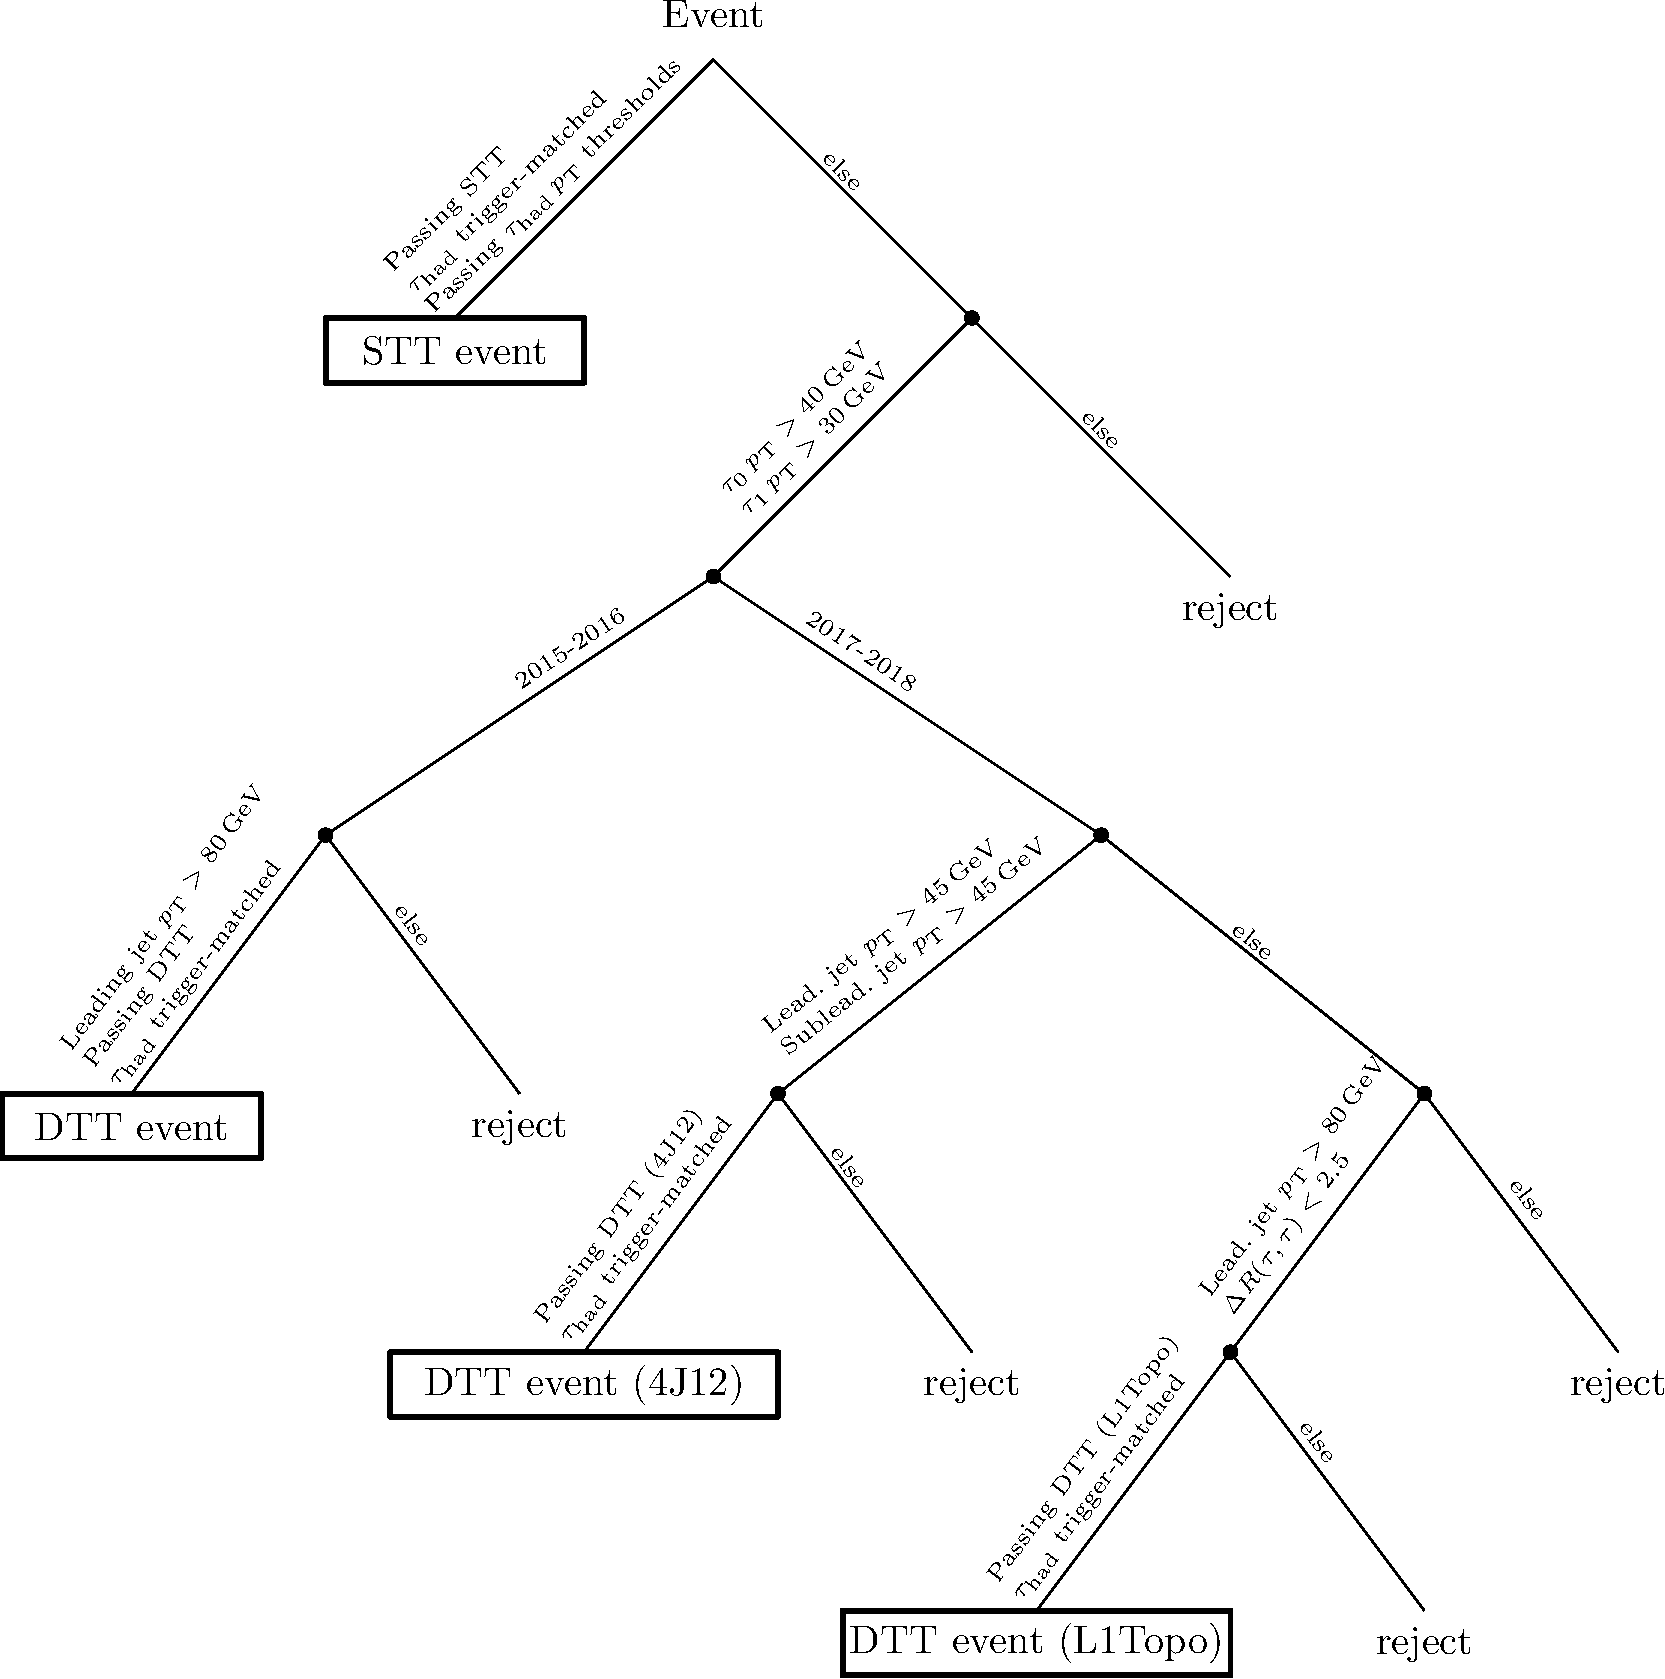
\includegraphics[width=0.8\textwidth]{figures/selection/HadHad_HH/trigger_flowchart_hadhad}
  \caption{Flowchart of the $\tauhad\tauhad$ trigger selection. ``Pass
    STT / DTT'' refers to checking whether the trigger selected the
    event (cf.~\Cref{tab:triggers_hadhad} for the triggers relevant
    for each run period).}
  \label{fig:hadhad_trigger_flowchart}
\end{figure}

A small inconsistency is present in the separation of the STT and DTT
trigger channels (c.f.\ first branching
in~\Cref{fig:hadhad_trigger_flowchart}). This is illustrated in the
following starting with the correct method that is used for the
sub-categorization of DTT events.

The categorization of DTT events is performed by first checking the
offline thresholds corresponding to the trigger of interest. Only if
these thresholds are fulfilled it is checked whether the trigger
selected the event and the reconstructed \tauhad are geometrically
matched to the HLT objects. If the offline thresholds are fulfilled
but the trigger did not select the event or the trigger-matching
failed, the event is rejected and not considered for any other
trigger-channel.

When distinguishing between STT and DTT categories this is not done
purely using offline reconstructed quantities since it is
simultaneously checked whether the event passes offline thresholds and
trigger-matching. This means that events that pass STT offline
thresholds but fail STT trigger-matching are still considered as
candidates in the DTT category (unlike the correct approach that is
used for DTT event sub-classification where these events are rejected
and not considered for further categorization). This would be
problematic when applying \tauhad trigger calibrations in the DTT
channel because there can be events that were explicitly checked to
fail STT-matching which violates the assumptions of the \tauhad
trigger calibration measurement. The fraction of events that pass the
STT thresholds but were not selected by the STT was checked and it was
found that only 0.1 to 0.2\,\% of events in the signal region are
affected. Therefore, this inconsistency has negligible effect on the
analysis.

More studies motivating the choices regarding the trigger strategy in
$bb\hadhad$ can be found in~\Cref{subsec:hadhad_trigger_studies}.


\subsection{Event cleaning}
\label{subsec:eventcleaning}
All events are subjected to the standard ATLAS event cleaning procedure, following the recommendations of the \href{https://twiki.cern.ch/twiki/bin/viewauth/Atlas/DataPreparationCheckListForPhysicsAnalysis}{\underline{DataPrep group}}.
Data events must be part of the runs listed in the GRLs as described in Section~\ref{sec:data}. 
A veto is applied to the following bad or corrupted events:
\begin{itemize}
\item LAr noise burst and data corruption (xAOD::EventInfo::LAr),
\item Tile corrupted events (xAOD::EventInfo::Tile),
\item events affected by the SCT recovery procedure for single event upsets (xAOD::EventInfo::SCT),
\item incomplete events (xAOD::EventInfo::Core).
\end{itemize}

Events are required to have a primary vertex with at least two associated tracks. The primary vertex is selected as the one with the largest $\sum \pT^2$, where the sum is over all tracks with transverse momentum \pt > 0.5 GeV that are associated with the vertex.

%\subsection{di-Higgs event selection}

%\subsubsection{\lephad event selection}
\subsection{\lephad event selection}
\label{subsec:selhh_lephad}
Event selection is applied that selects events compatible with containing a $\ell\tau_{\mathrm{had}}\bbbar$ final state. This selection forms the signal region containing the set of events that are used for the fit of the MVA discriminant distributions as described in Section~\ref{sec:fit}. Events must meet the following requirements
(using the object definitions described in section \ref{sec:reco}):
\begin{itemize}
\item SLT events:
	\begin{itemize}
		\item Exactly one electron passing the `tight' identification criteria, or one muon passing the `medium' identification criteria 
		%(that also includes a requirement that the muon must have | $\eta$ | < 2.5), 
		with $\pT$ 1 $\GeV$ above the corresponding trigger threshold used in that data-taking period.
		\item Exactly one hadronic $\tau$ with \pT > 20 $\GeV$ and |$\eta$| < 2.3.
		\item At least two jets in the event with \pT > 45 (20) $\GeV$ for the leading (sub-leading) jet.
	\end{itemize}
\item LTT events:
	\begin{itemize}
		\item Exactly one electron passing the `tight' identification criteria and with \pT > 18 $\GeV$, or one
 		muon passing the `medium' identification criteria with \pT > 15 GeV. 
		An upper limit on the \pT corresponding to the equivalent SLT thresholds for that data-taking period is applied.
		Electrons are required to pass the `tight' isolation working point for ETT, 
		since the single-leg electron trigger SFs are not available for loose iso electrons.  
		(Tightening the electron isolation cut leads to 4.7\% (4.1\%) lost in ggF (VBF) non-resonant signal yields in the LTT category.) 
		\item Exactly one hadronic $\tau$ with \pT > 30 $\GeV$ and |$\eta$| < 2.3.
		\item The \pT thresholds on the leading and sub-leading jets depend on the 
		corresponding trigger applied. Trigger list can be found in \ref{sec:lephadtrigger}.
		\begin{itemize}
			\item For the $e\tau$ trigger (2017-2018), since OR of two triggers are applied, the one that requires lower jet \pT threshold is prioritized.
			\item For the $\mu\tau$ trigger (2017-2018), two different jet \pT thresholds are applied for $\pT^{\tau}$ > 40 $\GeV$ and 30 < $\pT^{\tau}$ < 40 $\GeV$ since different triggers are applied for these two regions.
			\item The \pT thresholds applied are as follows:
				 \begin{itemize}
					\item If the applied trigger is seeded by L1 with J25 requirement, 
					at least two jets in the event with \pT > 80 (20) $\GeV$ for the leading (sub-leading) jet are required.
					\item If the applied trigger is seeded by L1 with 3J12 or 4J12 requirement,
					at least two jets in the event with \pT > 45 $\GeV$ are required.
					\item If there is no jet requirement at L1, at least two jets in the event with \pT > 45 (20) $\GeV$ for the leading (sub-leading) jets are required.
				\end{itemize}
		\end{itemize}
	\end{itemize}
\item No other electrons or muons in the event.
\item Opposite-sign charge between the $\tau$ and the light lepton ($e/\mu$).
\item Exactly two $b$-tagged jets (using DL1r 77\% working point).
\item The invariant mass of the \bbbar system, \mbb, is required to be < 150 GeV.
\item The invariant mass of the di-$\tau$ system (calculated using the Missing Mass Calculator (MMC) \cite{Elagin:2010aw}),
$\mMMC_{\tau\tau}$, must be > 60 $\GeV$.
\end{itemize}

\begin{figure}
\centering
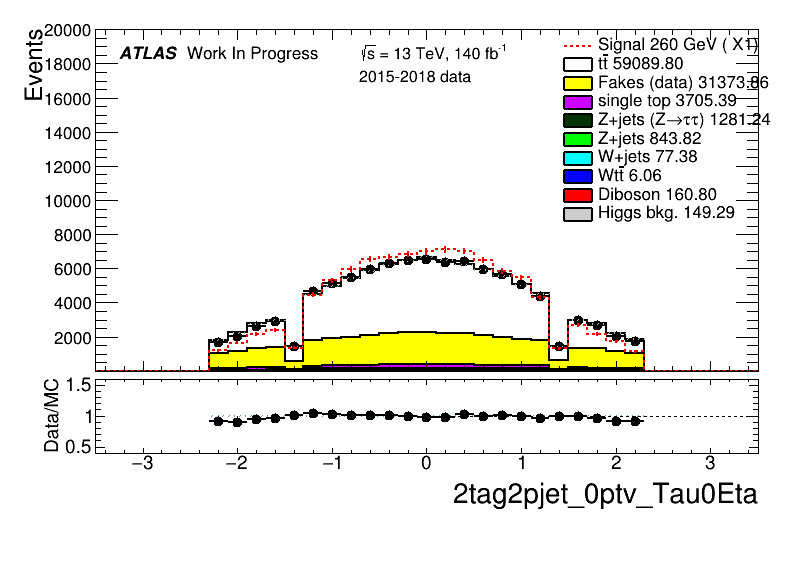
\includegraphics[width=.45\textwidth]{figures/selection/2tag2pjet_0ptv_Tau0Eta_SR_ALLFAKES_SLT_ALL_NR_TRBins.png}
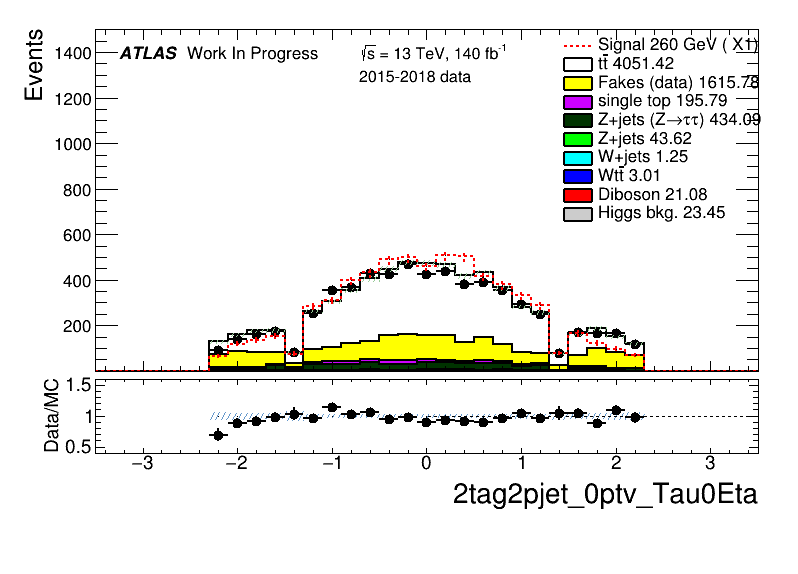
\includegraphics[width=.45\textwidth]{figures/selection/2tag2pjet_0ptv_Tau0Eta_SR_ALLFAKES_LTT_ALL_NR_TRBins.png} \\
\caption{Plots of $\tau$ $\eta$, demonstrating that the signal (scaled to the integral of the background) peaks more sharply at zero than the background in the \lephad channel. Included for the (left) single lepton trigger channel and (right) lepton-plus-tau trigger channel.}
\label{fig:tau_eta_23}
\end{figure}

The selection for $\tau$ $|\eta|$ to be less than 2.3 differs from the selection in the hadhad channel, and has been chosen as an analysis optimization choice from previous rounds of the analysis.  As you can see in Fig.~\ref{fig:tau_eta_23}, the signal is expected to peak more sharply at low |$\eta$| than the background, so the cut at 2.3 is expected to provide a modest background reduction.

	
  
\begin{table}
    \centering
    \scriptsize
    \begin{tabular}{|c|c|c|c|c|}
    	\hline
	\hline
	SampleName & Entries & Integral & Error & Error/Integ.\\

	\hline
 	\hline    
 	hhttbbggFSM     &151522 &5.86759 & 0.0179841&0.31\% \\ 
	hhttbbVBFSM	   	&36457  & 0.20024&0.0012615&0.63\% \\
	Hhhbbtautau251	& 22541 &	60.5803  & 0.416596	& 0.69\% \\
	Hhhbbtautau260	& 22252 &	60.8690  & 0.422004	& 0.69\% \\
	Hhhbbtautau280	& 24595 &	67.9352  & 0.447715	& 0.66\% \\
	Hhhbbtautau300	& 18398 &	77.1913  & 0.588118	& 0.76\% \\
	Hhhbbtautau325	& 20904 &	90.9350  & 0.649871	& 0.71\% \\
	Hhhbbtautau350	& 23593 &	106.391  & 0.716122	& 0.67\% \\
	Hhhbbtautau400	& 29280 &	140.007  & 0.845998	& 0.60\% \\
	Hhhbbtautau450	& 34665 &	175.289  & 0.973111	& 0.56\% \\
	Hhhbbtautau500	& 21332 &	210.657  & 1.48889	& 0.71\% \\
	Hhhbbtautau550	& 23571 &	240.878  & 1.62159	& 0.67\% \\
	Hhhbbtautau600	& 25917 &	273.858  & 1.75829	& 0.64\% \\
	Hhhbbtautau700	& 29596 &	327.036  & 1.96578	& 0.60\% \\
	Hhhbbtautau800	& 32606 &	374.464  & 2.14260	& 0.57\% \\
	Hhhbbtautau900	& 34392 &	405.559  & 2.26269	& 0.56\% \\
	Hhhbbtautau1000	& 35119 &	425.155  & 2.34509	& 0.55\% \\
	Hhhbbtautau1100	& 44157 &	416.216  & 2.04469	& 0.49\% \\
	Hhhbbtautau1200	& 32337 &	386.871  & 2.43156	& 0.63\% \\
	Hhhbbtautau1400	& 25539 &	251.079  & 1.62164	& 0.65\% \\
	Hhhbbtautau1600	& 14421 &	160.598  & 1.39334	& 0.87\% \\
	\hline
	
	Fake     	  &	2054613  & 35834.2   & 116.072    &	0.32\% \\
	ttbar     	  &	490058    & 61707.2   & 91.4456    & 0.15\% \\
	stopWt 	   &	25910      & 3068.72   & 19.8006    & 0.65\% \\
	stopt   	   &	5798        & 597.841   & 11.146      &	1.86\% \\
	stops 	   &	1450        & 38.0965   & 1.0672      &	 2.80\% \\
	Zbb 		   &	17645      & 577.445   & 18.6845    &	 3.24\% \\
	Zbc 		   &	1467        & 57.1754   & 7.31240    &	 12.79\% \\
	Zbl 	            &	1006        & 39.4660   & 5.89920    &	 14.95\% \\
	Zcc 	            &	278 	        & 63.3618   & 16.3586    &	 25.82\% \\
	Zcl	            &	135          & 23.1748   & 10.38491   & 44.81\% \\
	Zl	            &	30            & 5.1560     & 2.5307       & 49.08\% \\
	Zttbb 	    &	21473      & 1034.74   & 19.7203     & 1.91\% \\
	Zttbc 	    &	1746        & 100.9634 & 7.84392     & 7.77\% \\
	Zttbl 		    &	1184        & 62.7492   & 6.58925     & 10.50\% \\
	Zttcc 	    &	608          & 118.2826 & 21.84047   & 18.46\% \\
	Zttcl		    &	216          & 12.6376   & 9.48049     & 75.02\% \\
	Zttl 		    &	122          & 15.5227   & 5.58566     & 35.98\% \\
	W 		    &	747          & 77.4938   & 8.40607     & 10.85\% \\
	DY                &	68            & 13.5159   & 3.40597     & 25.20\% \\
	Wtt               &	76            & 5.51685   & 0.816626   & 14.80\% \\
	DYtt              &	9              & 2.6588     & 1.72628     & 64.93\% \\
	WW              &	110          & 14.0836   & 2.19759     & 15.60\% \\
	WZ               &	1992        & 60.1072   & 2.73295     & 4.55\% \\
	ZZ 		    &	6754        & 84.6051   & 2.08094     & 2.46\% \\
	VBFHtautau &	933          & 1.4224     & 0.0491357 & 3.45\% \\
	ggFHtautau  &	2159        & 17.1723   & 0.443422   & 2.58\% \\
	ggZHtautau  &	838          & 2.87863   & 0.10284     & 3.57\% \\
	ZHtautau      &	1923        & 8.497219 & 0.206055   & 2.42\% \\
	WHtautau     &	92            & 0.714224 & 0.0805373 & 11.28\% \\
	ZHbb            &	88889      & 23.4744   & 0.252781   & 1.08\% \\
	WHbb           &	6054        & 6.94652   & 0.143376   & 2.06\% \\
	ttH                &	37692      & 58.0919   & 0.312495   & 0.54\% \\
	\hline
	
 	\hline
	total bkg  & 2772080 & 103734.0 & &\\
	data         & 98456     & 98456	& &\\
 	\hline
 	\hline
	  
      \end{tabular}
      \caption{Pre-fit event yields in the di-Higgs $bb\lephad$ SLT signal region for the data, background and signal. Here, Zttjj represents the processes as $Z\rightarrow\tau\tau + jj$,
      whereas Zjj represents  $Z\rightarrow ee/\mu\mu + jj$.}
      \label{tab:LepHadSLTYields}
\end{table}
  

\begin{table}
    \centering
    \scriptsize
    \begin{tabular}{|c|c|c|c|c|}
	
	\hline
	\hline
	SampleName & Entries & Integral & Error & Error/Integ.\\
	
	\hline
	\hline
	hhttbbggFSM    &35045	 &1.416186  &	0.008843 & 0.62\%\\	
	hhttbbVBFSM	   &10188  	&0.054756 	&0.00063987&1.17\% \\
  	Hhhbbtautau251 & 6815	 & 17.9678  & 0.224815 & 1.25\% \\
  	Hhhbbtautau260 & 6930	 & 18.4965  & 0.22967   & 1.24\% \\
	Hhhbbtautau280 & 8145	 & 22.2273  & 0.25376   & 1.14\% \\
	Hhhbbtautau300 & 6319 	& 26.4815  & 0.34358   & 	1.30\% \\
 	Hhhbbtautau325 & 7085 	& 30.8642  & 0.37816   & 	1.23\% \\
  	Hhhbbtautau350 & 7896 	& 35.9407  & 0.41597   & 	1.16\% \\
  	Hhhbbtautau400 & 8780 	& 42.5375  & 0.46722   & 	1.10\% \\
        Hhhbbtautau450  & 9303 	& 47.4140  & 0.50589  &  	1.07\% \\
	Hhhbbtautau500  & 5177 	& 51.6729  & 0.73896  & 	1.43\% \\
	Hhhbbtautau550  & 5123 	& 53.3731  & 0.76570  & 	1.43\% \\
	Hhhbbtautau600   & 5026 	& 53.8328 & 0.78163  & 	1.45\% \\
	Hhhbbtautau700   &	4699	 & 52.8369 & 0.79526 & 	1.51\% \\
	Hhhbbtautau800   &	4534	 & 52.7574 & 0.80652 & 	1.53\% \\
	Hhhbbtautau900   &	4285	 & 51.5907 & 0.81138 & 	1.57\% \\
	Hhhbbtautau1000 &	3820	 & 47.4054 & 0.78933 & 	1.67\% \\
	Hhhbbtautau1100 &	4436	 & 42.8090 & 0.66043 & 	1.54\% \\
 	Hhhbbtautau1200 &	2878	 & 33.9867 & 0.71017 & 	2.09\% \\	
	Hhhbbtautau1400 &	2264	 & 22.6836 & 0.49023 & 	2.16\% \\
 	Hhhbbtautau1600 &	1412	 & 16.0911 & 0.44594 & 	2.77\% \\
  	\hline
  
  	Fake 	&  39074	&	2146.46	&	41.7068  &	1.94\% \\
	ttbar           & 32873 &	4213.13     &	24.0372  &	0.57\% \\
	stopWt       & 1408   &	169.8852   &	4.70386  &	2.77\% \\
	stopt          & 246     &	26.1433     &	2.43237  &	9.30\% \\
	stops          & 61      &	1.6708       &	0.22960  &	13.74\% \\
	Zbb            & 1230   &	33.5952     &	3.98824  &	11.87\% \\
	Zbc            & 92       &	3.7974       &	0.82655  &	21.77\% \\
	Zbl             & 58       &	1.2151       &	0.88899  &	73.16\% \\
	Zcc            & 14       &	4.08084     &	3.10603  &	76.11\% \\
	Zcl             & 5         &	0.8519       &	0.60706  &	71.26\% \\
	Zl               & 2         &	0.0510206 &	0.03608  &	70.71\% \\
	Zttbb          & 7271   &	352.1282   &	10.66373&	3.03\% \\
	Zttbc           & 634    &	34.7063     &	4.07317  &	11.74\% \\
	Zttbl            & 406    &	27.8580     &	3.23106  &	11.60\% \\	
	Zttcc           & 174    &	28.1896     &	7.23583  &	25.67\% \\	
	Zttcl            & 86      &	8.4072       &	4.96063  &	59.00\% \\
	Zttl              & 57      &	10.8339     &	7.33489  &	67.70\% \\
	W                & 16      &	1.3289       &	0.34673  &	26.09\% \\	
	DY              & 6         &	0.5694       &	0.28426  &	49.93\% \\
	Wtt              & 22      &	2.69751     &	0.96584  &	35.81\% \\
	DYtt             & 3        &	0.2597       &	0.16896  &	65.06\% \\
	WW             & 4        &	0.4316       &	0.23477  &	54.40\% \\
	WZ               & 119   &	3.56164     &	0.53030  &	14.89\% \\
	ZZ                & 1360 &	17.2611     &	0.94440  &	5.47\% \\
	VBFHtautau & 235   &	0.3715       &	0.02506  &	6.74\% \\	
	ggFHtautau  & 461   &	4.5775       &	0.24447  &	5.34\% \\
	ggZHtautau  & 218   &	0.7408       &	0.05219  &	7.05\% \\
	ZHtautau      & 458   &	2.1790       &	0.10592  &	4.86\% \\
	WHtautau     & 23     &	0.1783       &	0.03965  &	22.23\% \\
 	ZHbb            & 16172&	5.3097       &	0.14934 &	 	2.81\% \\
	WHbb           & 82     &	0.1735       &	0.02609 &		15.04\% \\
	ttH                 & 5121 &	8.1182       &	0.11766 &		1.45\% \\
	\hline

        \hline
	total bkg 	&	107991  &	   7110.77 &  & \\		
	data		& 	6351      &    6351 	&  &   \\
	\hline
	\hline

    \end{tabular}
    \caption{Pre-fit event yields in the di-Higgs $bb\lephad$ LTT signal region for signal, data and background. Here, Zttjj represents the processes as $Z\rightarrow\tau\tau + jj$, 
    whereas Zjj represents  $Z\rightarrow ee/\mu\mu + jj$.}
    \label{tab:LepHadLTTYields}
\end{table}

The event yields after applying the $bb\lephad$ SLT and LTT event selections are shown in Table \ref{tab:LepHadSLTYields} and \ref{tab:LepHadLTTYields} for signal, data and background. 

Figures~\ref{fig:LepHadAccEffSLT} and \ref{fig:LepHadAccEffLTT} show the acceptance times efficiency of the \lephad SLT and LTT channel selections, respectively, for the di-Higgs resonant signals as a function of the resonance mass. \begin{figure}
\centering
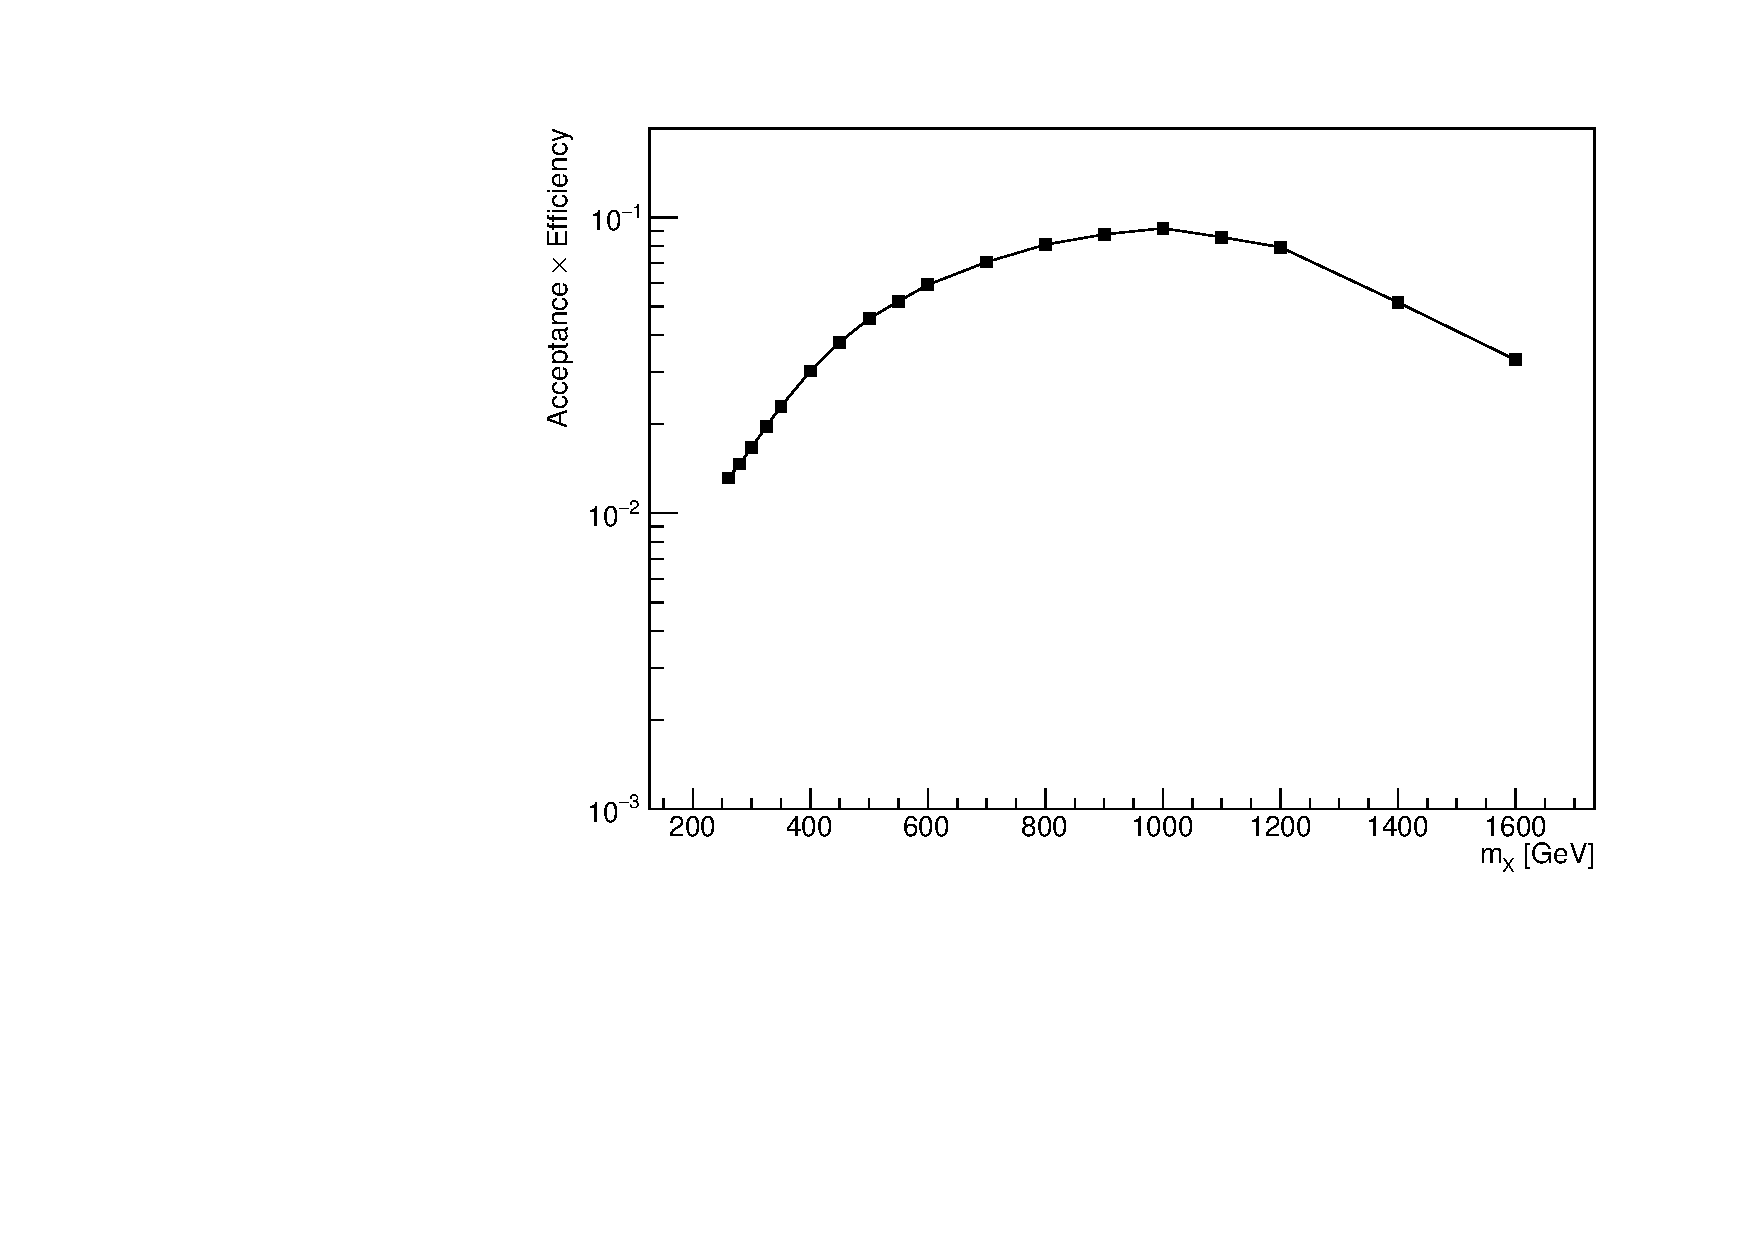
\includegraphics[width=.65\textwidth]{figures/selection/LepHad_HH/SLT_AccEff.pdf}
\caption{Acceptance times efficiency of the \lephad SLT channel selection for the di-Higgs resonant signals as a function of the resonance mass.}
\label{fig:LepHadAccEffSLT}
\end{figure}

\begin{figure}
\centering
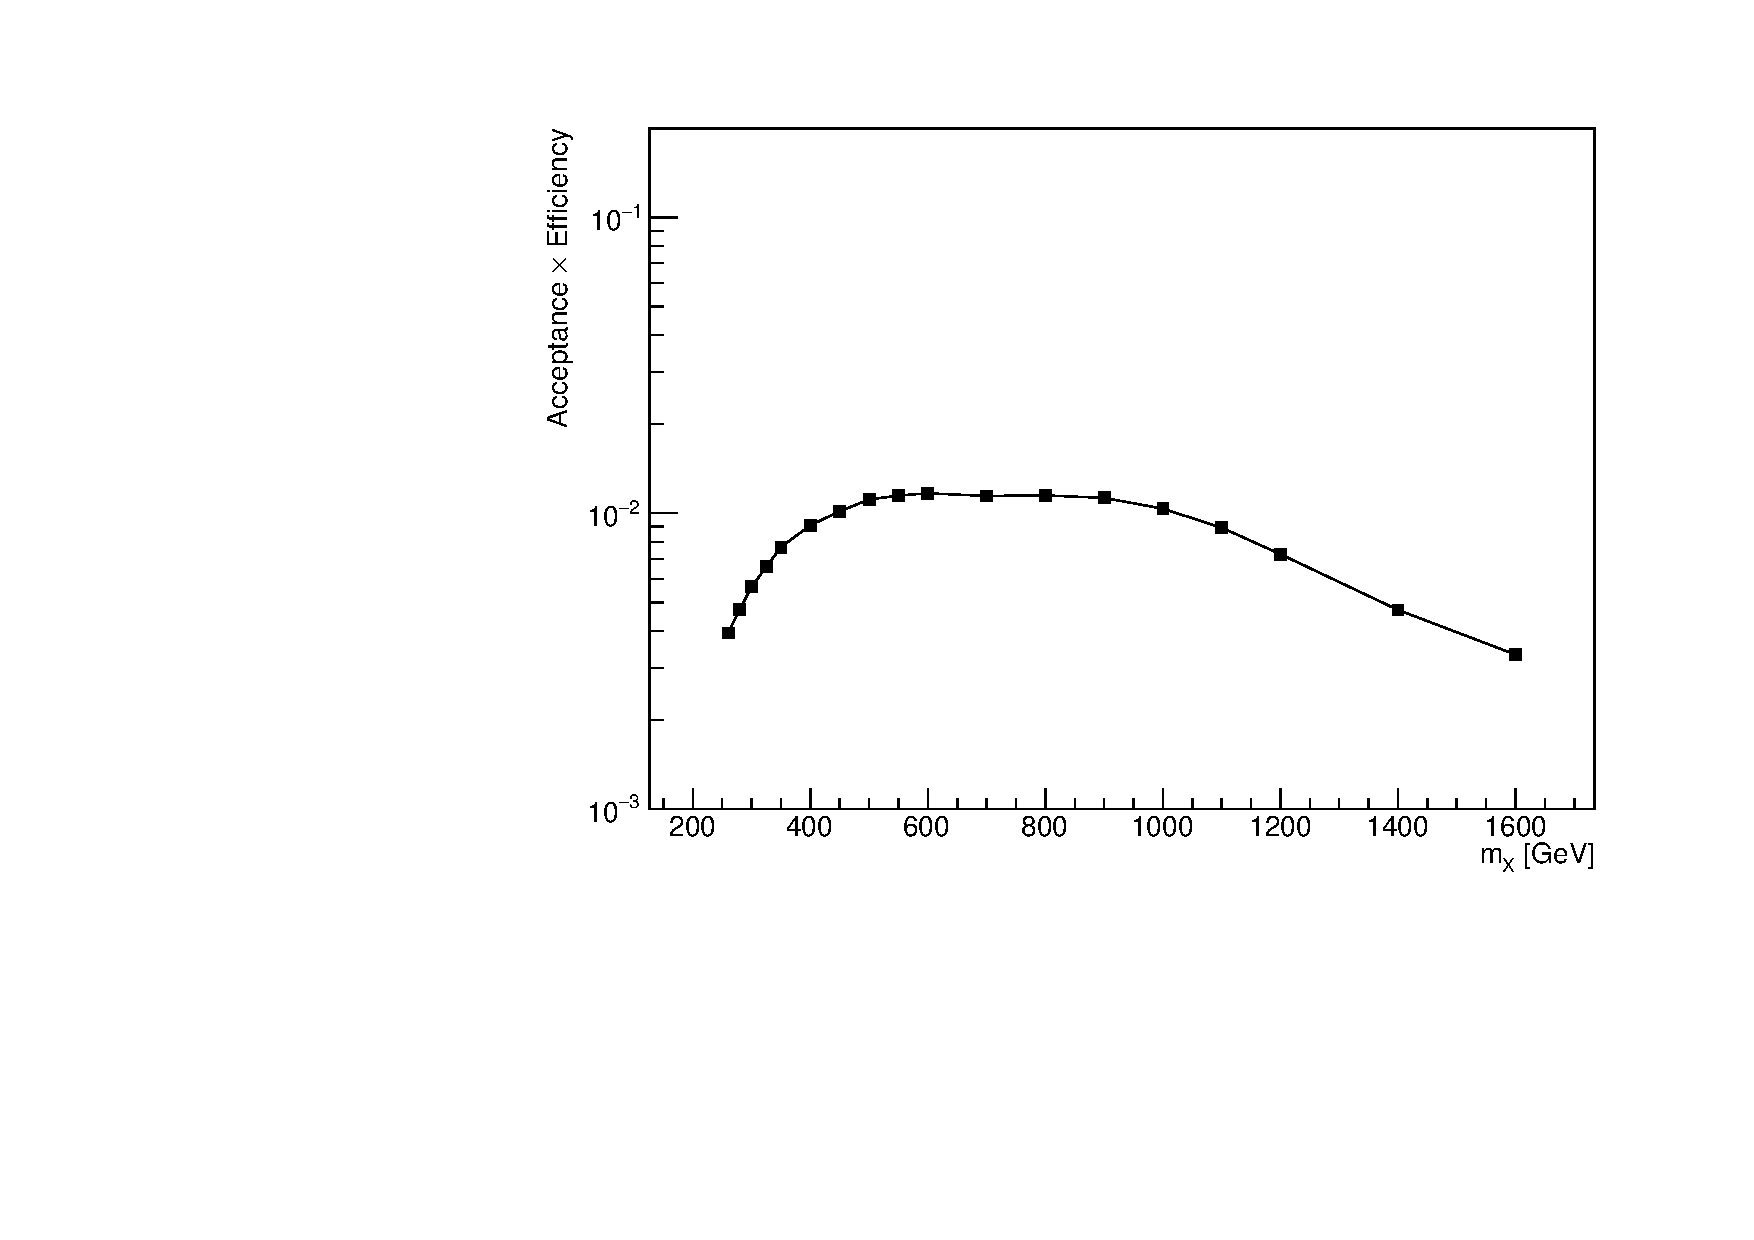
\includegraphics[width=.65\textwidth]{figures/selection/LepHad_HH/LTT_AccEff.pdf}
\caption{Acceptance times efficiency of the \lephad LTT channel selection for the di-Higgs resonant signals as a function of the resonance mass.}
\label{fig:LepHadAccEffLTT}
\end{figure}

\begin{landscape}
\begin{table}
\centering

\begin{tabular}{|c|cc|cc|cc|}
\hline
Description & \multicolumn{2}{c|}{Number of events} & \multicolumn{2}{c|}{Efficiency [\%]} & \multicolumn{2}{c|}{Relative Efficiency [\%] }\\
\hline
& SLT & LTT & SLT &  LTT &  SLT &  LTT \\
\hline
$HH$ & \multicolumn{2}{c|}{4313.87} & \multicolumn{2}{c|}{x} & \multicolumn{2}{c|}{x} \\
$HH\rightarrow bb\tau\tau$ & \multicolumn{2}{c|}{315.23} & \multicolumn{2}{c|}{x} & \multicolumn{2}{c|}{x} \\
$HH\rightarrow bb\tau_{lep}\tau_{h}$ & \multicolumn{2}{c|}{143.82} & \multicolumn{2}{c|}{100.00} & \multicolumn{2}{c|}{100.00} \\
Generator filter & \multicolumn{2}{c|}{91.98} &  \multicolumn{2}{c|}{63.96} &  \multicolumn{2}{c|}{63.96} \\
Derivation skimming & \multicolumn{2}{c|}{71.94} & \multicolumn{2}{c|}{50.02} & \multicolumn{2}{c|}{78.21} \\
Object preselection & \multicolumn{2}{c|}{27.53} & \multicolumn{2}{c|}{19.14} & \multicolumn{2}{c|}{38.26} \\
\hline
Trigger selection (online+offline) & \multicolumn{2}{c|}{21.68} & \multicolumn{2}{c|}{15.08} & \multicolumn{2}{c|}{100.00} \\ 
Trigger category & 16.79 & 4.90 & 11.67 & 3.40 & 77.42 & 22.58 \\
\hline
Random tau selection & 16.79 & 4.90 & 11.67 & 3.40 & 100.00 & 100.00 \\
Object selection ($n_\tau=2$, further requirements on jets and tau-jet OLR) & 15.43 & 4.48 & 10.73 & 3.11 & 91.93 & 91.51 \\
Lepton, $\tau$,trigger eff weight &14.25&	4.26&	9.91	&2.96	&92.34&	95.01\\
$\tau$ $\eta$ Cut & 14.01 & 4.16 & 9.74 & 2.90 & 98.35 & 98.55 \\
Trigger Specific \pT cut & 13.66	&3.30	&9.50	&2.29	&97.50	&79.24 \\
Opposite charge sign & 13.48 & 3.27	&9.37&	2.28&	98.62&	99.21\\
\hline
Both jets are $b$-tagged & 6.28 & 1.52	&4.36&	1.06&	46.58&	46.35 \\
MMC > 60 GeV & 6.18 & 1.50	&4.30&	1.04&	98.52&	98.62 \\
$m_{bb} < 150$ GeV & 5.87 & 1.42	&4.08&	0.98&	94.87	&94.63 \\
\hline
\end{tabular}
\caption{Non-resonant \lephad SM ggF signal cutflow (Powheg+Pythia8).}
\label{tab:SMHH_lephad_cutflow}
\end{table}
\end{landscape}

\begin{landscape}
    \begin{table}
    \centering
\begin{tabular}{|c|cc|cc|cc|}
 \hline
 Description & \multicolumn{2}{c|}{Number of events} & \multicolumn{2}{c|}{Efficiency [\%]} & \multicolumn{2}{c|}{Relative Efficiency [\%] }\\
 \hline
 & SLT & LTT & SLT &  LTT &  SLT &  LTT \\
 \hline
 $HH$ & \multicolumn{2}{c|}{239.798} &	\multicolumn{2}{c|}{x}   & \multicolumn{2}{c|}{x}  \\
 $HH\rightarrow bb\tau\tau$ & \multicolumn{2}{c|}{17.523}  &  \multicolumn{2}{c|}{x}   & \multicolumn{2}{c|}{x} \\
 $HH\rightarrow bb\tau_{lep\tau_{h}}$ & \multicolumn{2}{c|}{7.995}   &  \multicolumn{2}{c|}{100.00} &   \multicolumn{2}{c|}{x} \\
 Generator filter & \multicolumn{2}{c|}{4.587}   &  \multicolumn{2}{c|}{57.38} &    \multicolumn{2}{c|}{57.38} 	 \\
 Derivation skimming & \multicolumn{2}{c|}{3.429}   &  \multicolumn{2}{c|}{42.89} &    \multicolumn{2}{c|}{74.75} 	 \\
 Object preselection & \multicolumn{2}{c|}{1.302}   &  \multicolumn{2}{c|}{16.29} &    \multicolumn{2}{c|}{37.97} 	 \\
 \hline
 Trigger selection (online+offline) & \multicolumn{2}{c|}{0.99}   &  \multicolumn{2}{c|}{12.39} &    \multicolumn{2}{c|}{76.11} 	 \\
 Trigger category & 0.736   &   0.255   &  9.20  & 3.19  &    70.41 &   24.40 \\
 \hline
 Random tau selection & 0.736   &   0.255   &  9.20  & 3.19  &    100.00    &   100.00 \\
 Object selection ($n_\tau=2$, further requirements on jets and tau-jet OLR) & 0.628   &   0.216   &  7.86  & 2.70  &    85.35 &   84.78 \\
 Lepton, $\tau$,trigger eff weight & 0.588   &   0.206   &  7.35  & 2.58  &    93.59 &   95.32 \\
 $\tau$ $\eta$ Cut & 0.572   &   0.182   &  7.15  & 2.28  &    97.26 &   88.42 \\
 Trigger Specific \pT cut & 0.540   &   0.147   &  6.76  & 1.84  &    94.49 &   80.93 \\
 Opposite charge sign & 0.531   &   0.146   &  6.64  & 1.83  &    98.31 &   99.03 \\
 \hline
 Both jets are $b$-tagged & 0.218   &   0.061   &  2.72  & 0.76  &    40.97 &   41.65 \\
 MMC > 60 GeV & 0.214   &   0.060   &  2.68  & 0.75  &    98.32 &   98.59 \\
 $m_{bb} < 150$ GeV & 0.204   &   0.057   &  2.55  & 0.71  &    95.17 &   94.57 \\
 \hline
 \end{tabular}
 \caption{Non-resonant \lephad SM VBF signal cutflow (Powheg+Pythia8).}
 \label{tab:SMHH_lephad_VBF_cutflow}
 \end{table}
 \end{landscape}
 
 \begin{landscape}
     \begin{table}
     \centering
 \begin{tabular}{|c|cc|cc|cc|}
     \hline
     Description & \multicolumn{2}{c|}{Number of events} & \multicolumn{2}{c|}{Efficiency [\%]} & \multicolumn{2}{c|}{Relative Efficiency [\%] }\\
     \hline
     & SLT & LTT & SLT &  LTT &  SLT &  LTT \\
     \hline
$HH$                                                                          &  \multicolumn{2}{c|}{138933.42} & 	 \multicolumn{2}{c|}{x} &  \multicolumn{2}{c|}{x}\\
$HH\rightarrow bb\tau\tau$                                                                        &  \multicolumn{2}{c|}{10152.37} &  \multicolumn{2}{c|}{x} &  \multicolumn{2}{c|}{x} \\
$HH\rightarrow bb\tau_{lep\tau_{h}}$                                                                        &  \multicolumn{2}{c|}{4632.02} & 		 \multicolumn{2}{c|}{100.00} &     \multicolumn{2}{c|}{x} \\
Generator filter                                                                          &  \multicolumn{2}{c|}{2418.50} & 		 \multicolumn{2}{c|}{52.21} & 		 \multicolumn{2}{c|}{52.21}\\
Derivation skimming                                                                       &  \multicolumn{2}{c|}{1731.94} & 		 \multicolumn{2}{c|}{37.39} & 		 \multicolumn{2}{c|}{71.61}\\
Object preselection                                                                       &  \multicolumn{2}{c|}{585.27} & 		 \multicolumn{2}{c|}{12.64} & 		 \multicolumn{2}{c|}{33.79} \\
\hline
Trigger selection (online+offline)                                                                        &  \multicolumn{2}{c|}{409.06} & 		 \multicolumn{2}{c|}{8.83} &  		 \multicolumn{2}{c|}{69.89}\\
Trigger category                                                                          & 279.01 & 	130.05 &    	6.02 &	2.81 &	67.29 &	31.36 \\
\hline
Random tau selection                                                                          & 279.01 & 	130.05 &    	6.02 &	2.81 &	100.00 &	100.00 \\
Object selection ($n_\tau=2$, further requirements on jets and tau-jet OLR)               & 247.43 & 	117.08 &    	5.34 &	2.53 &	88.68 &	90.02 \\
Lepton, $\tau$,trigger eff weight                                                                         & 237.84 & 	112.24 &    	5.13 &	2.42 &	96.12 &	95.87 \\
$\tau$ $\eta$ Cut                                                                         & 232.58 & 	99.56 & 	5.02 &	2.15 &	97.79 &	88.70 \\
Trigger Specific \pT cut                                                                          & 204.50 & 	66.30 & 	4.41 &	1.43 &	87.92 &	66.60 \\
Opposite charge sign                                                                          & 201.58 & 	65.74 & 	4.35 &	1.42 &	98.57 &	99.15 \\
\hline
Both jets are $b$-tagged                                                                          & 82.56 & 	28.27 & 	1.78 &	0.61 &	40.96 &	43.01 \\
MMC > 60 GeV                                                                          & 82.21 & 	28.20 & 	1.77 &	0.61 &	99.57 &	99.74 \\
$m_{bb} < 150$ GeV                                                                        & 77.19 & 	26.33 & 	1.67 &	0.57 &	93.90 &	93.39 \\
\hline
\end{tabular}
\caption{300 GeV mass point resonant \lephad signal cutflow (Madgraph+Herwig7).}
\label{tab:SMHH_lephad_resonant_300_cutflow}
\end{table}
\end{landscape}

\begin{landscape}
    \begin{table}
    \centering
\begin{tabular}{|c|cc|cc|cc|}
    \hline
    Description & \multicolumn{2}{c|}{Number of events} & \multicolumn{2}{c|}{Efficiency [\%]} & \multicolumn{2}{c|}{Relative Efficiency [\%] }\\
    \hline
    & SLT & LTT & SLT &  LTT &  SLT &  LTT \\
    \hline
$HH$              &  \multicolumn{2}{c|}{138933.42} &		 \multicolumn{2}{c|}{x}	&	 \multicolumn{2}{c|}{x} \\
$HH\rightarrow bb\tau\tau$              &  \multicolumn{2}{c|}{10152.37} &		 \multicolumn{2}{c|}{x}	&	 \multicolumn{2}{c|}{x} \\
$HH\rightarrow bb\tau_{lep\tau_{h}}$              &  \multicolumn{2}{c|}{4632.02} &		 \multicolumn{2}{c|}{100.00}	&	 \multicolumn{2}{c|}{x} \\
Generator filter              &  \multicolumn{2}{c|}{3352.31} &		 \multicolumn{2}{c|}{72.37}	&	 \multicolumn{2}{c|}{72.37} \\
Derivation skimming              &  \multicolumn{2}{c|}{2595.68} &		 \multicolumn{2}{c|}{56.04}	&	 \multicolumn{2}{c|}{77.43} \\
Object preselection              &  \multicolumn{2}{c|}{1030.53} &		 \multicolumn{2}{c|}{22.25}	&	 \multicolumn{2}{c|}{39.70} \\
\hline	
Trigger selection (online+offline)              &  \multicolumn{2}{c|}{826.51} &		 \multicolumn{2}{c|}{17.84}	&	 \multicolumn{2}{c|}{80.20} \\
Trigger category              & 640.82 &	185.69 &	13.83 &	4.01 &	71.03 &	20.58 \\
\hline
Random tau selection              & 640.82 &	185.69 &	13.83 &	4.01 &	100.00 &	100.00 \\
Object selection ($n_\tau=2$, further requirements on jets and tau-jet OLR)              & 599.70 &	173.81 &	12.95 &	3.75 &	93.58 &	93.61 \\
Lepton, $\tau$,trigger eff weight              & 519.90 &	151.90 &	11.22 &	3.28 &	86.69 &	87.39 \\
$\tau$ $\eta$ Cut              & 510.61 &	129.54 &	11.02 &	2.80 &	98.21 &	85.28 \\
Trigger Specific \pT cut              & 503.77 &	121.67 &	10.88 &	2.63 &	98.66 &	93.93 \\
Opposite charge sign              & 497.22 &	120.84 &	10.73 &	2.61 &	98.70 &	99.32 \\
\hline
Both jets are $b$-tagged              & 225.07 &	55.13 &	4.86 &	1.19 &	45.26 &	45.63 \\
MMC > 60 GeV              & 222.13 &	54.33 &	4.80 &	1.17 &	98.70 &	98.54 \\
$m_{bb} < 150$ GeV              & 210.66 &	51.29 &	4.55 &	1.11 &	94.83 &	94.41 \\
\hline
\end{tabular}
\caption{500 GeV mass point resonant \lephad signal cutflow (Madgraph+Herwig7).}
\label{tab:SMHH_lephad_resonant_500_cutflow}
\end{table}
\end{landscape}


\begin{landscape}
    \begin{table}
    \centering
\begin{tabular}{|c|cc|cc|cc|}
    \hline
    Description & \multicolumn{2}{c|}{Number of events} & \multicolumn{2}{c|}{Efficiency [\%]} & \multicolumn{2}{c|}{Relative Efficiency [\%] }\\
    \hline
    & SLT & LTT & SLT &  LTT &  SLT &  LTT \\
    \hline
$HH$       & \multicolumn{2}{c|}{138933.42} &		\multicolumn{2}{c|}{x}	&	\multicolumn{2}{c|}{x}	\\
$HH\rightarrow bb\tau\tau$       & \multicolumn{2}{c|}{10152.37} &		\multicolumn{2}{c|}{x}	&	\multicolumn{2}{c|}{x}	\\
$HH\rightarrow bb\tau_{lep\tau_{h}}$       & \multicolumn{2}{c|}{4632.02} &		\multicolumn{2}{c|}{100.00}	&	\multicolumn{2}{c|}{x}	\\
Generator filter       & \multicolumn{2}{c|}{3811.20} &		\multicolumn{2}{c|}{82.28}	&	\multicolumn{2}{c|}{82.28}	\\
Derivation skimming       & \multicolumn{2}{c|}{3129.45} &		\multicolumn{2}{c|}{67.56}	&	\multicolumn{2}{c|}{82.11}	\\
Object preselection       & \multicolumn{2}{c|}{1397.05} &		\multicolumn{2}{c|}{30.16}	&	\multicolumn{2}{c|}{44.64}	\\
\hline
Trigger selection (online+offline)       & \multicolumn{2}{c|}{1195.31} &		\multicolumn{2}{c|}{25.81}	&	\multicolumn{2}{c|}{85.56}	\\
Trigger category       & 1039.84 & 	155.47 & 	22.45 & 	3.36 &	76.81  	& 11.48 \\
\hline
Random tau selection       & 1039.84 & 	155.47 & 	22.45 & 	3.36 &	100.00  	& 100.00 \\
Object selection ($n_\tau=2$, further requirements on jets and tau-jet OLR)       & 1016.54 & 	151.13 & 	21.95 & 	3.26 &	97.76  	& 97.21 \\
Lepton, $\tau$,trigger eff weight       & 942.87 & 	141.71 & 	20.36 & 	3.06 &	92.75  	& 93.77 \\
$\tau$ $\eta$ Cut       & 933.70 & 	109.03 & 	20.16 & 	2.35 &	99.03  	& 76.94 \\
Trigger Specific \pT cut       & 931.28 & 	107.74 & 	20.11 & 	2.33 &	99.74  	& 98.82 \\
Opposite charge sign       & 918.39 & 	106.69 & 	19.83 & 	2.30 &	98.62  	& 99.03 \\
\hline
Both jets are $b$-tagged       & 462.52 & 	52.28 & 	9.99 & 	1.13 &	50.36  	& 49.00 \\
MMC > 60 GeV       & 447.51 & 	49.34 & 	9.66 & 	1.07 &	96.76  	& 94.37 \\
$m_{bb} < 150$ GeV       & 425.16 & 	47.16 & 	9.18 & 	1.02 &	95.00  	& 95.58 \\
\hline
\end{tabular}
\caption{1000 GeV mass point resonant \lephad signal cutflow (Madgraph+Herwig7).}
\label{tab:SMHH_lephad_resonant_1000_cutflow}
\end{table}
\end{landscape}


The non-resonant \lephad SM ggF signal cutflow is shown in \cref{tab:SMHH_lephad_cutflow}. 
The cutflow table starts with the theoretical yileds of the ggF di-Higgs production, followed by 
the yields in the \bbtt decay and \lephad channel. 
The generator filter cut is done in the MC generation.
The derivation skimming cut is done in the AOD to DAOD process of the data. 
The object preselection selection cut is done in the DAOD to CxAOD process to 
apply loose cuts on the physical objects. 
The trigger selection (online+offline) cut is done to select events triggered by the SLT and the
LTT triggers, followed by more requirements on the physical objects. 
Then the efficiency of the physical objects weight is applied. 
Then we require the $\eta$ of the hadronic $\tau$ to be smaller than 2.3. 
In the next cut we apply \pt cut with exactly 1 GeV greater than the \pt requirements
in the trigger selection. 
The we require the lepton and the hadronic $\tau$ to have opposite signs, and both of the
jets to be b-tagged at DL1r 77\% working point. Finally we require the mass of the 
reconstructed $Z$ boson to be greater than 60 GeV and the mass of the two b-jets to be
smaller than 150 GeV.


The acceptance times efficiency for the SM ggF signal in the \lephad channel is 4.08\% for the SLT channel and 0.985\% for the LTT channel.
In addition, the non-resonant \lephad SM VBF signal cutflow is shown in \cref{tab:SMHH_lephad_VBF_cutflow}. The acceptance times efficiency for the VBF SLT channel is 2.50\% and for the LTT channel is 0.685\%. 

To demonstrate the modeling of the events after this selection and that there is no significant mismodeling due to the $\tau$, electron or muon, and L1 jet trigger requirements, distributions are included to show the $\tau$ $p_T$ and $\eta$, the lepton (electron or muon) $p_T$ and $\eta$ (Fig.~\ref{fig:lh_taulepsel}), and the jet $p_T$ and $\eta$ both over the full dataset and for each year (Fig.~\ref{fig:lh_jetpteta}) since the jet requirements differ across data periods.  The most notable features from the jet requirements can be seen in the 2015-2016 data plot, where the leading $p_T$ jet is required to have $p_T > 80$~GeV, and the shoulder at 45~\GeV\ observed in later years. 

\begin{figure}
\centering
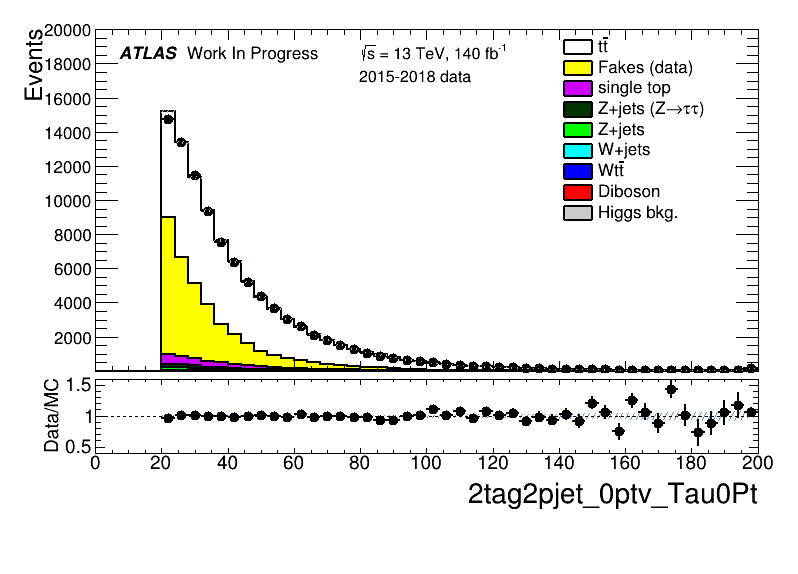
\includegraphics[width=.45\textwidth]{figures/selection/LepHad_HH/2tag2pjet_0ptv_Tau0Pt_SR_ALLFAKES_SLT_ALL_NR_TRBins.png}
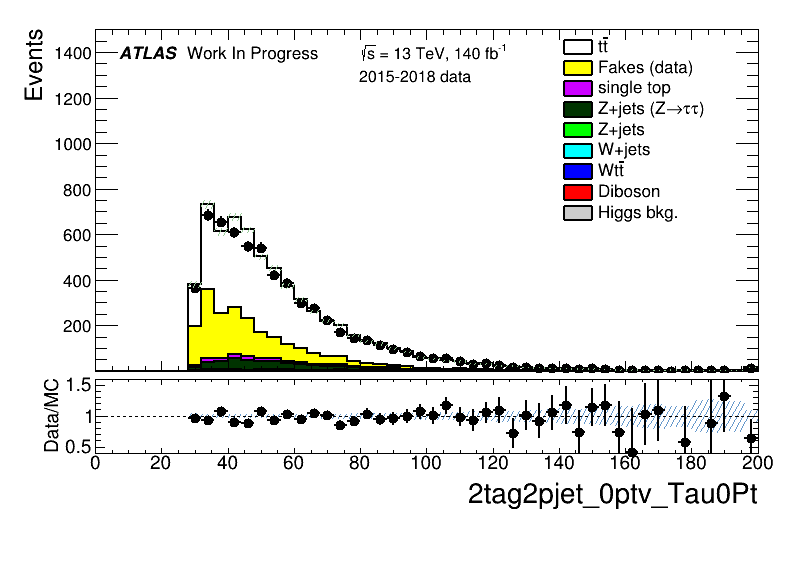
\includegraphics[width=.45\textwidth]{figures/selection/LepHad_HH/2tag2pjet_0ptv_Tau0Pt_SR_ALLFAKES_LTT_ALL_NR_TRBins.png} \\
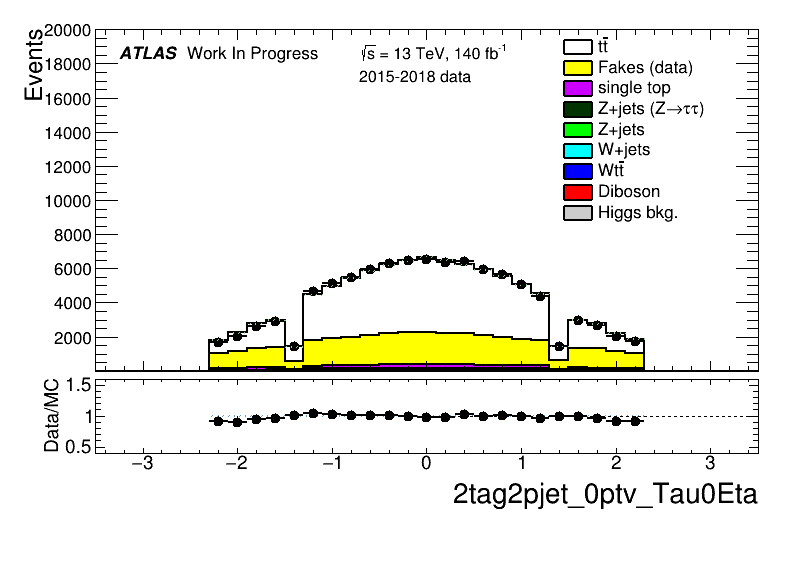
\includegraphics[width=.45\textwidth]{figures/selection/LepHad_HH/2tag2pjet_0ptv_Tau0Eta_SR_ALLFAKES_SLT_ALL_NR_TRBins.png}
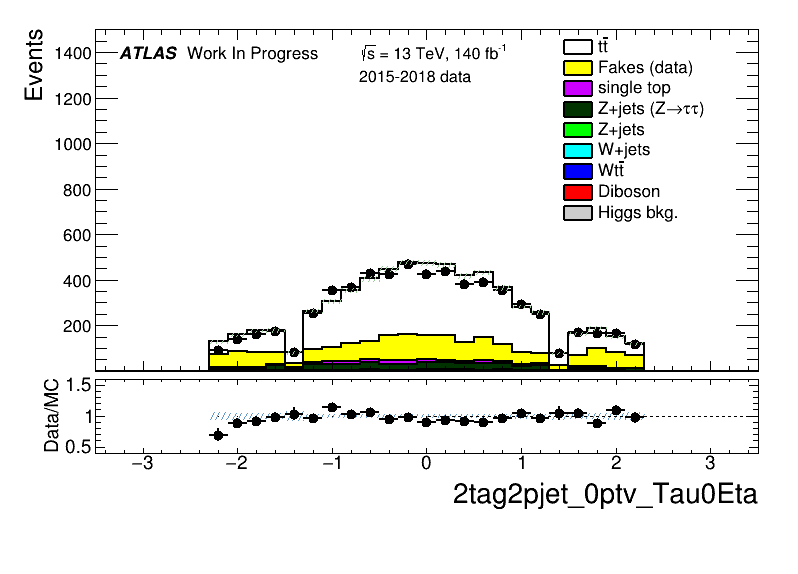
\includegraphics[width=.45\textwidth]{figures/selection/LepHad_HH/2tag2pjet_0ptv_Tau0Eta_SR_ALLFAKES_LTT_ALL_NR_TRBins.png} \\
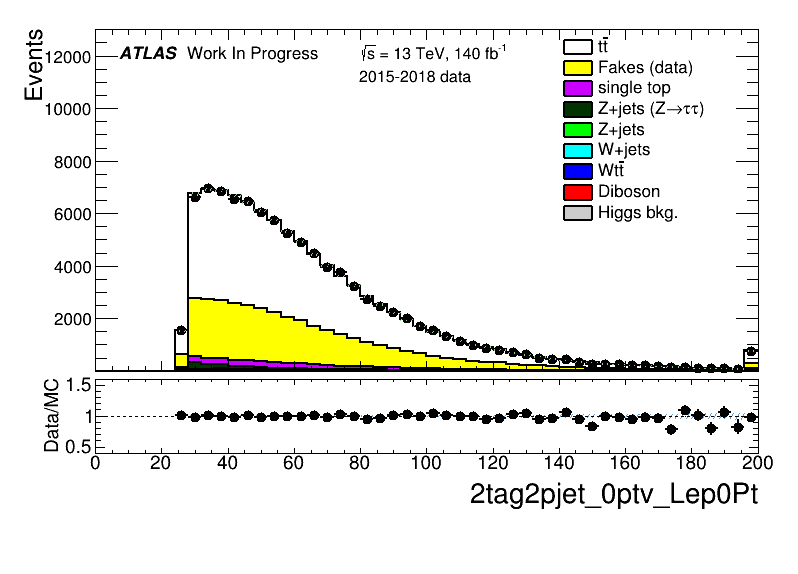
\includegraphics[width=.45\textwidth]{figures/selection/LepHad_HH/2tag2pjet_0ptv_Lep0Pt_SR_ALLFAKES_SLT_ALL_NR_TRBins.png}
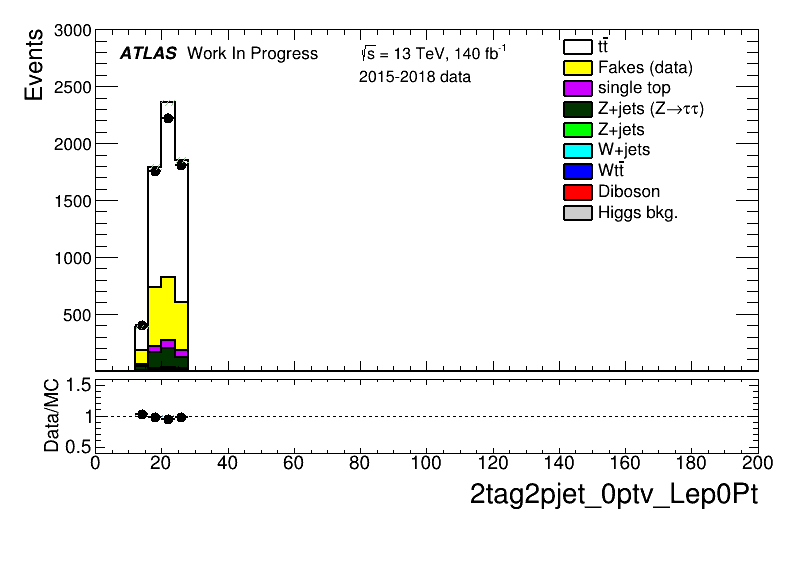
\includegraphics[width=.45\textwidth]{figures/selection/LepHad_HH/2tag2pjet_0ptv_Lep0Pt_SR_ALLFAKES_LTT_ALL_NR_TRBins.png} \\
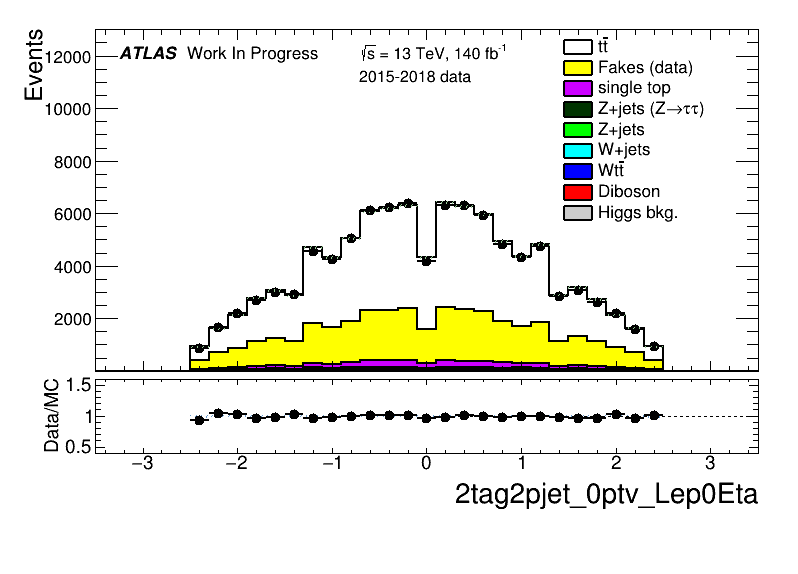
\includegraphics[width=.45\textwidth]{figures/selection/LepHad_HH/2tag2pjet_0ptv_Lep0Eta_SR_ALLFAKES_SLT_ALL_NR_TRBins.png}
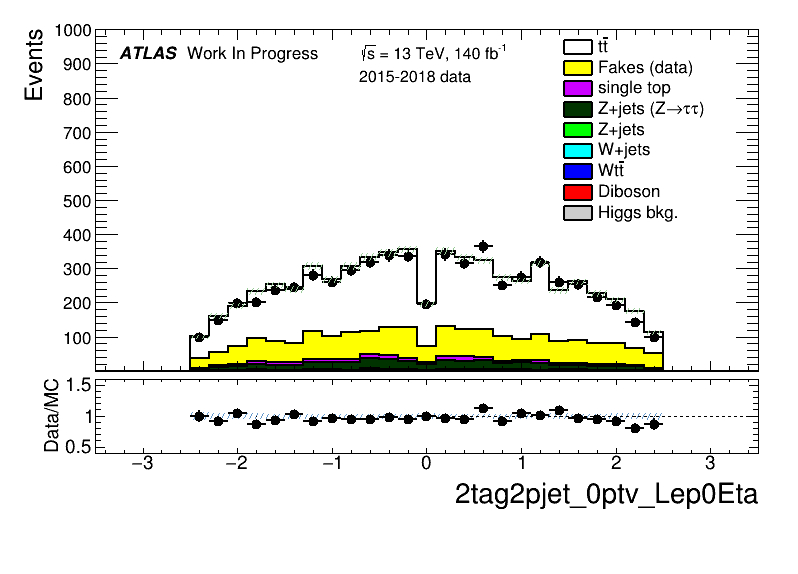
\includegraphics[width=.45\textwidth]{figures/selection/LepHad_HH/2tag2pjet_0ptv_Lep0Eta_SR_ALLFAKES_LTT_ALL_NR_TRBins.png} \\
\caption{Plots of (top row) $\tau$ $p_T$, (second row) $\tau$ $\eta$, (third row) lepton (electron or muon) $p_T$ and (bottom) $\eta$,  for the (left) SLT and (right) LTT trigger channels.}
\label{fig:lh_taulepsel}
\end{figure}


\begin{figure}
\centering
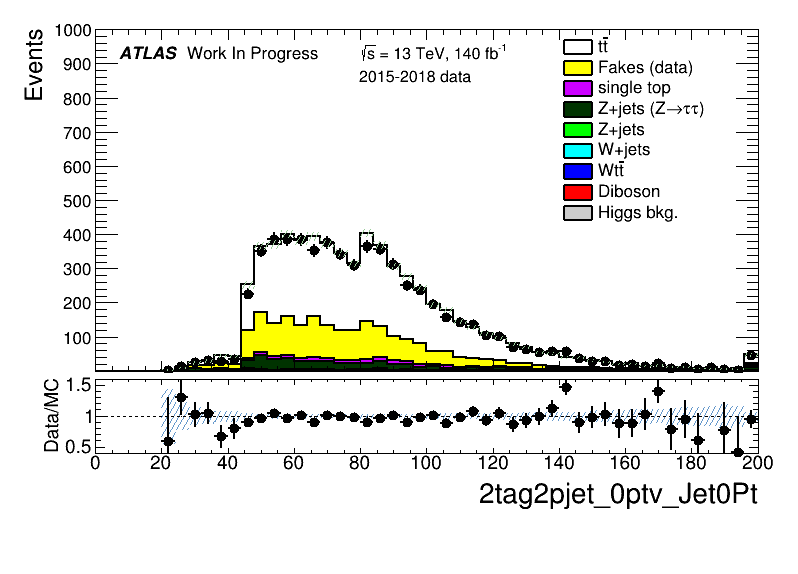
\includegraphics[width=.24\textwidth]{figures/selection/LepHad_HH/2tag2pjet_0ptv_Jet0Pt_SR_ALLFAKES_LTT_ALL_NR_TRBins.png} 
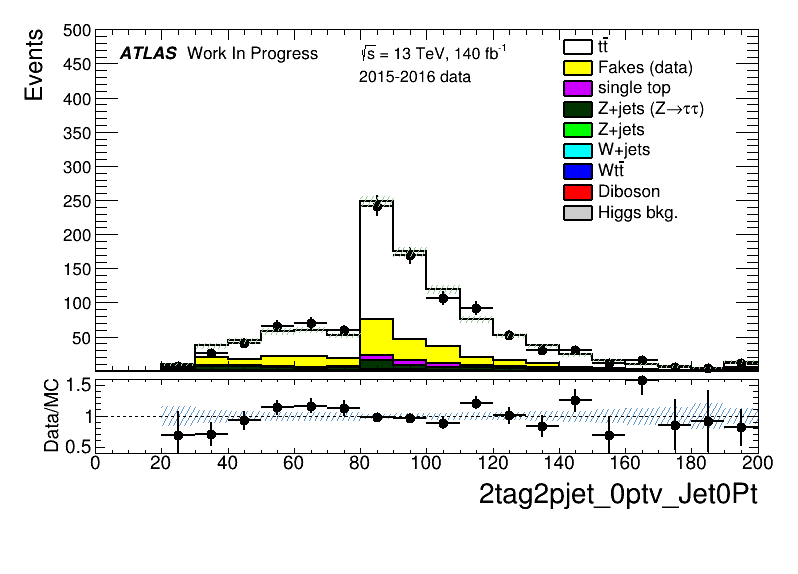
\includegraphics[width=.24\textwidth]{figures/selection/LepHad_HH/2tag2pjet_0ptv_Jet0Pt_SR_ALLFAKES_LTT_2016_TRBins.png} 
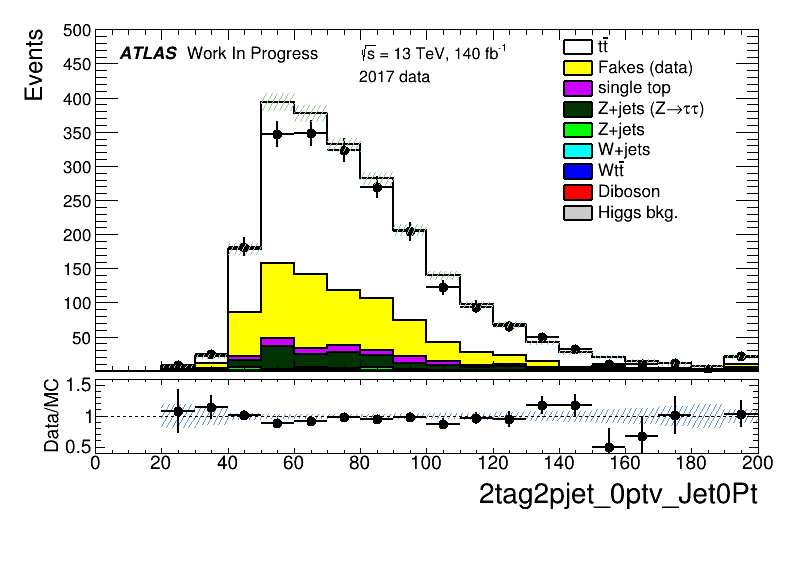
\includegraphics[width=.24\textwidth]{figures/selection/LepHad_HH/2tag2pjet_0ptv_Jet0Pt_SR_ALLFAKES_LTT_2017_TRBins.png} 
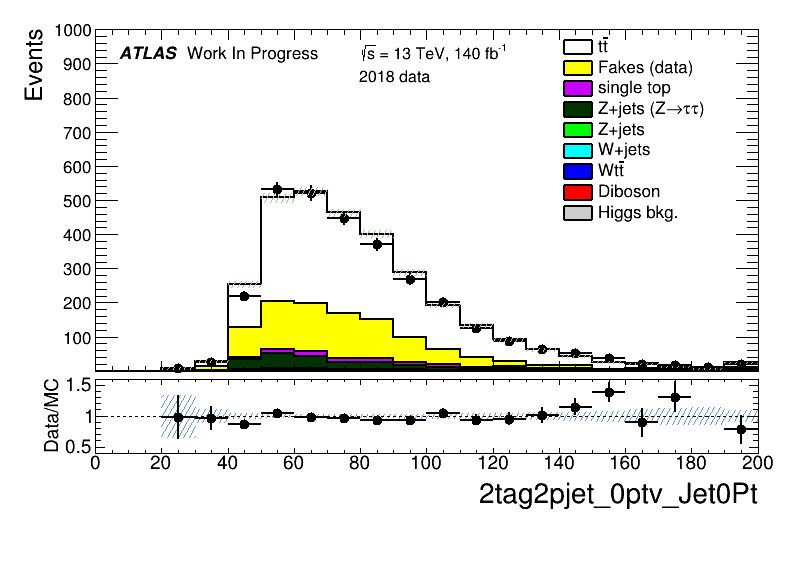
\includegraphics[width=.24\textwidth]{figures/selection/LepHad_HH/2tag2pjet_0ptv_Jet0Pt_SR_ALLFAKES_LTT_2018_TRBins.png} \\
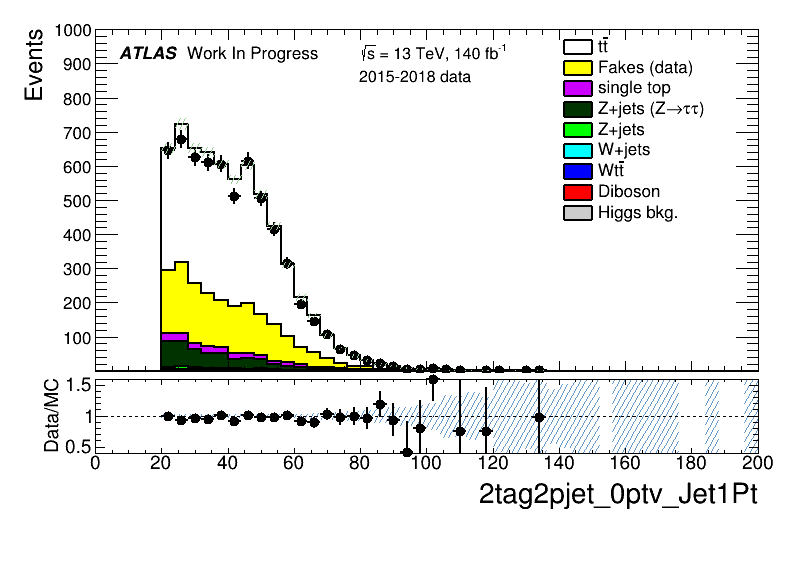
\includegraphics[width=.24\textwidth]{figures/selection/LepHad_HH/2tag2pjet_0ptv_Jet1Pt_SR_ALLFAKES_LTT_ALL_NR_TRBins.png}
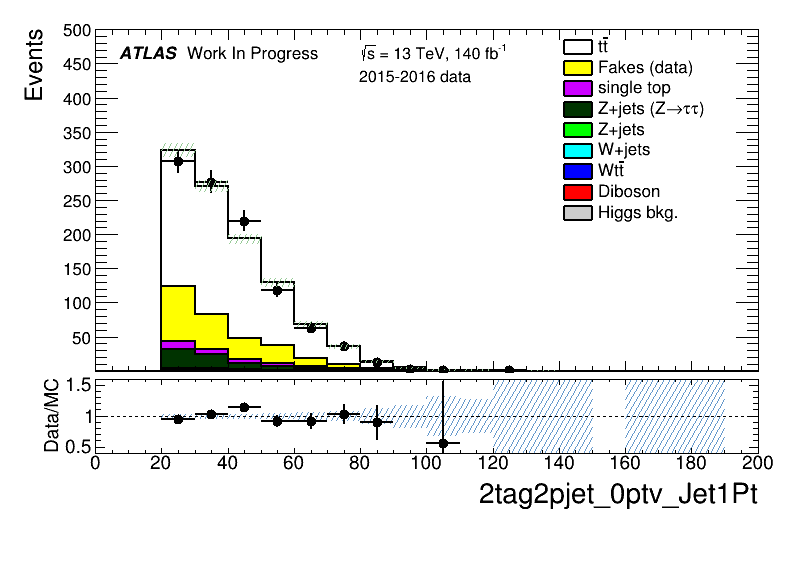
\includegraphics[width=.24\textwidth]{figures/selection/LepHad_HH/2tag2pjet_0ptv_Jet1Pt_SR_ALLFAKES_LTT_2016_TRBins.png}
 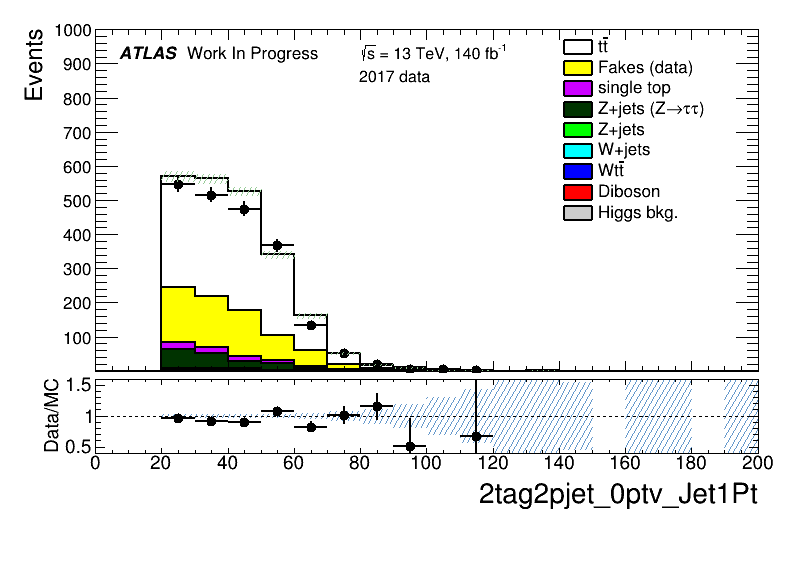
\includegraphics[width=.24\textwidth]{figures/selection/LepHad_HH/2tag2pjet_0ptv_Jet1Pt_SR_ALLFAKES_LTT_2017_TRBins.png}
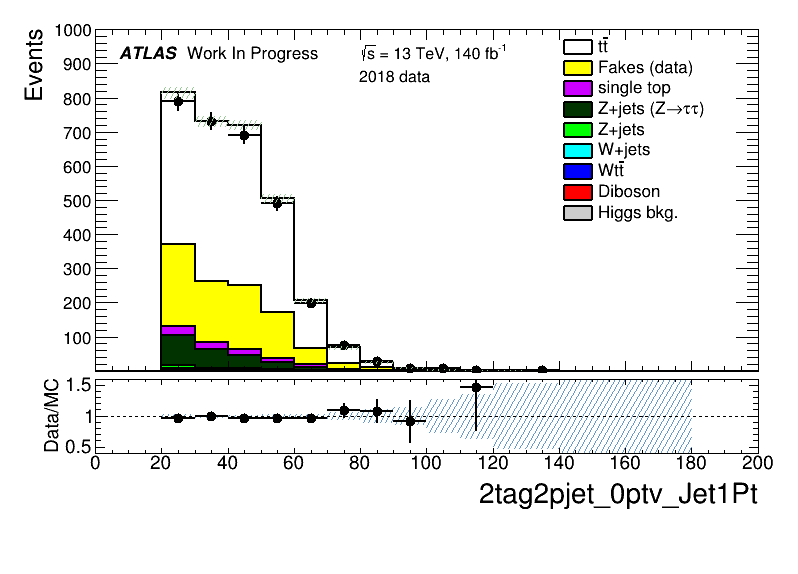
\includegraphics[width=.24\textwidth]{figures/selection/LepHad_HH/2tag2pjet_0ptv_Jet1Pt_SR_ALLFAKES_LTT_2018_TRBins.png} \\
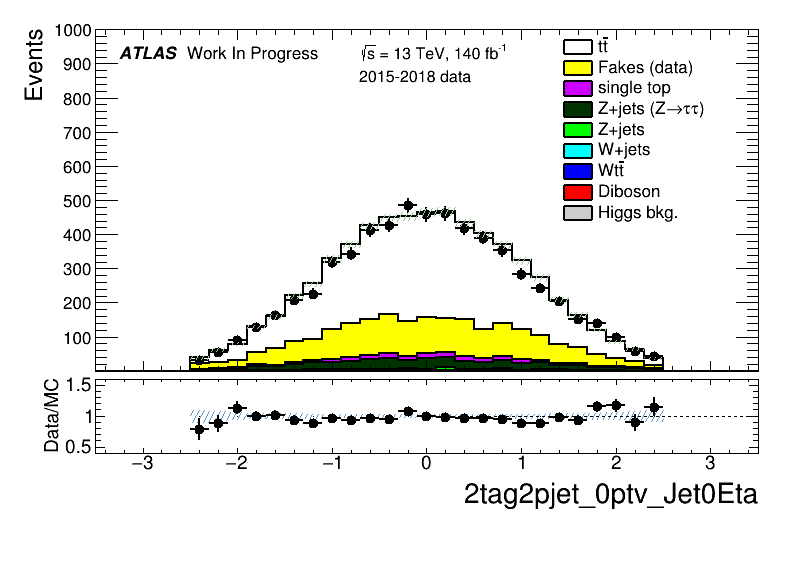
\includegraphics[width=.24\textwidth]{figures/selection/LepHad_HH/2tag2pjet_0ptv_Jet0Eta_SR_ALLFAKES_LTT_ALL_NR_TRBins.png} 
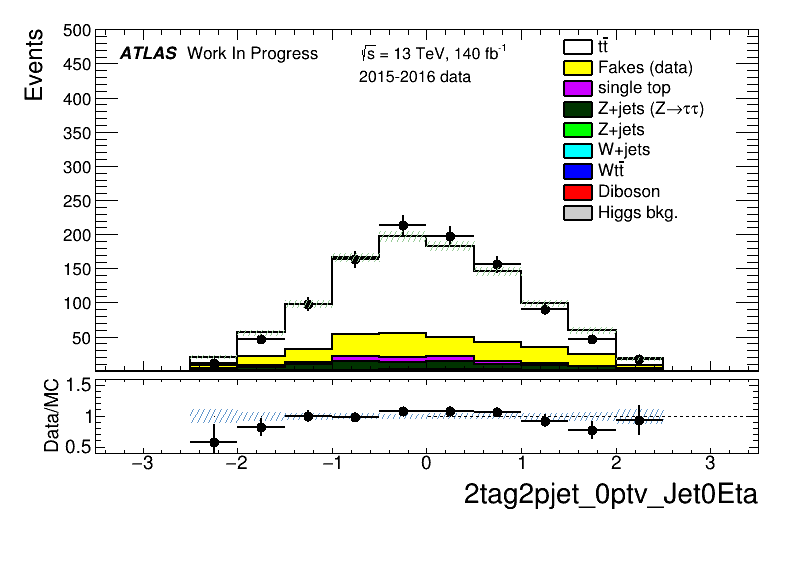
\includegraphics[width=.24\textwidth]{figures/selection/LepHad_HH/2tag2pjet_0ptv_Jet0Eta_SR_ALLFAKES_LTT_2016_TRBins.png} 
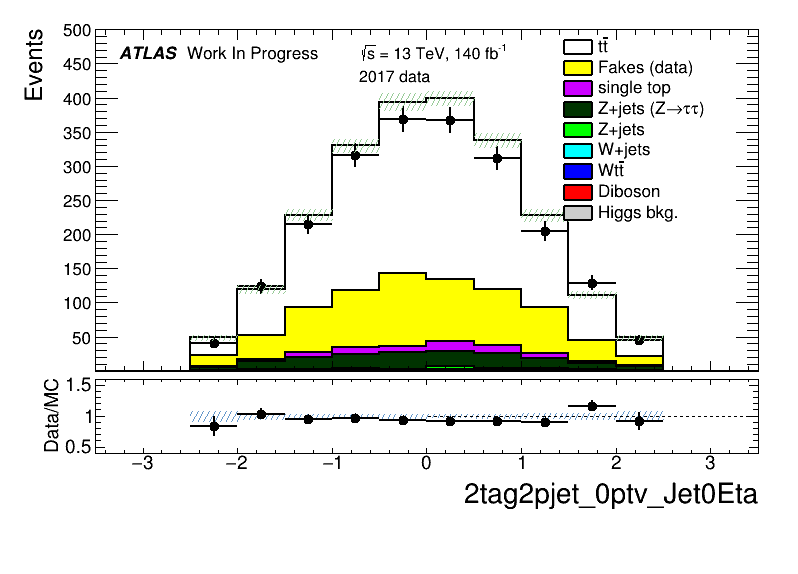
\includegraphics[width=.24\textwidth]{figures/selection/LepHad_HH/2tag2pjet_0ptv_Jet0Eta_SR_ALLFAKES_LTT_2017_TRBins.png} 
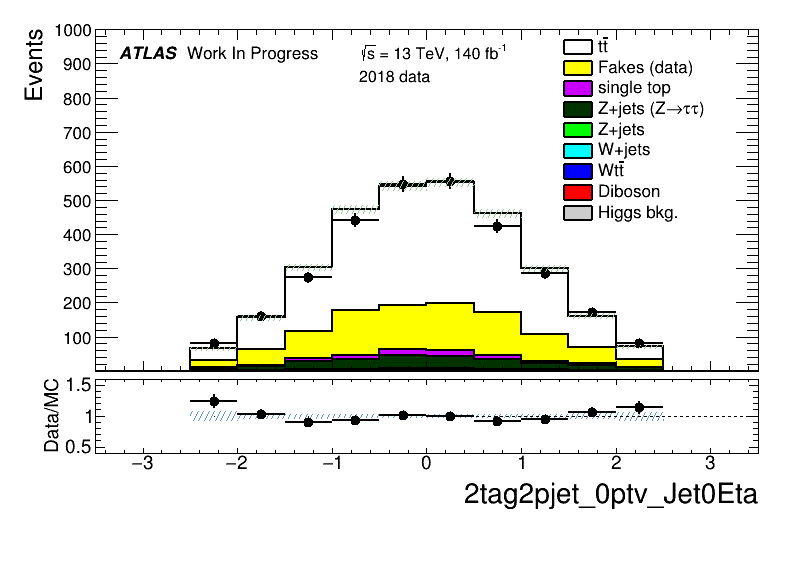
\includegraphics[width=.24\textwidth]{figures/selection/LepHad_HH/2tag2pjet_0ptv_Jet0Eta_SR_ALLFAKES_LTT_2018_TRBins.png} \\
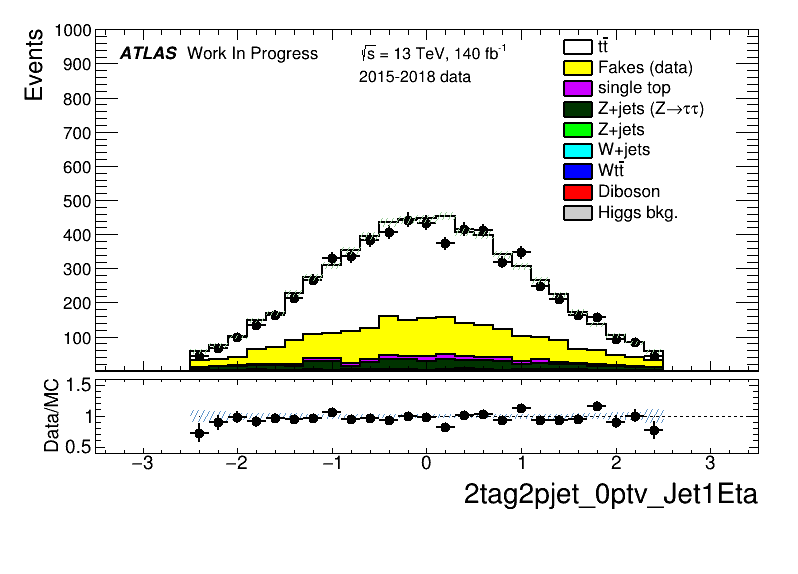
\includegraphics[width=.24\textwidth]{figures/selection/LepHad_HH/2tag2pjet_0ptv_Jet1Eta_SR_ALLFAKES_LTT_ALL_NR_TRBins.png}
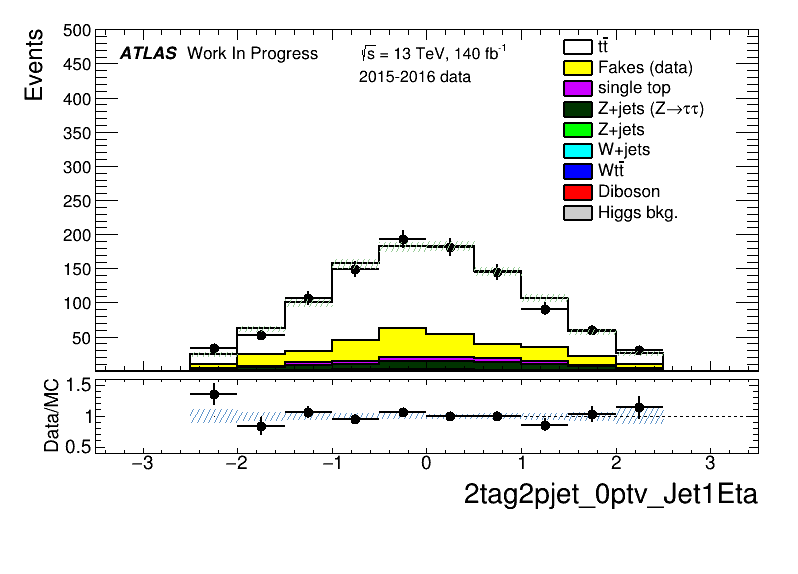
\includegraphics[width=.24\textwidth]{figures/selection/LepHad_HH/2tag2pjet_0ptv_Jet1Eta_SR_ALLFAKES_LTT_2016_TRBins.png}
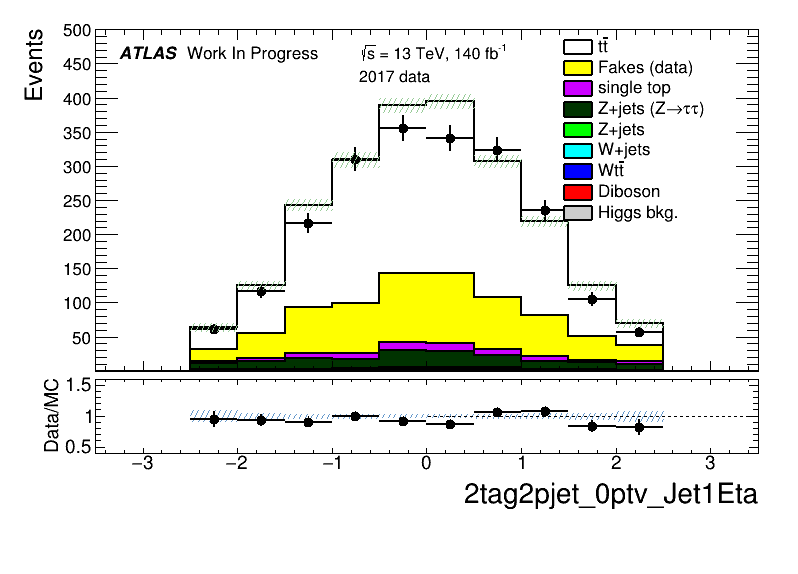
\includegraphics[width=.24\textwidth]{figures/selection/LepHad_HH/2tag2pjet_0ptv_Jet1Eta_SR_ALLFAKES_LTT_2017_TRBins.png}
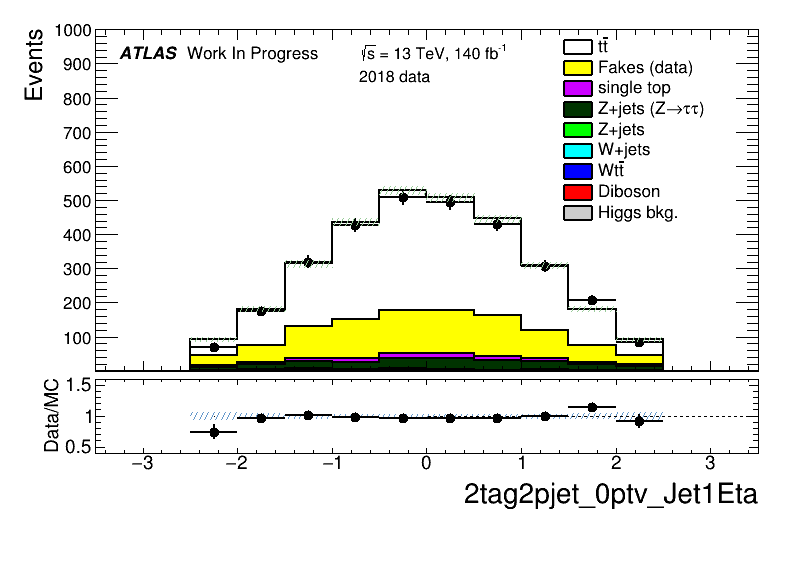
\includegraphics[width=.24\textwidth]{figures/selection/LepHad_HH/2tag2pjet_0ptv_Jet1Eta_SR_ALLFAKES_LTT_2018_TRBins.png}
\caption{Plots of jet $p_T$ and $\eta$ for the LTT trigger channels, specifically the $p_T$ of the (1st row) leading $p_T$ $b$-tagged jet, the (2nd row) second leading $p_T$ $b$-tagged jet, $\eta$ of the (3rd row) leading $p_T$ $b$-tagged jet, and the (4th row) second leading $p_T$ $b$-tagged jet. Shown are the total combined dataset (1st column), the 2015-2016 dataset (2nd column), the 2017 dataset (3rd column) and 2018 dataset (last column). Discontinuities correspond to the offline cuts required by trigger requirements at 80 GeV and 45 GeV for particular data periods.}
\label{fig:lh_jetpteta}
\end{figure}



\FloatBarrier

%\subsubsection{\hadhad event selection}
\subsection{\hadhad event selection}
\label{subsec:selhh_hadhad}
Selections are applied to selects events compatible with containing a $bb\tau_{had}\tau_{had}$ final state. This selection forms the signal region containing the set of events that are used for the fit of the MVA discriminant distributions as described in Section~\ref{sec:fit}. 

All events passing the trigger selection must then meet the following requirements (using the object definitions described in Section~\ref{sec:reco}):

\begin{itemize}
\item At least two jets;
\item Exactly two $\tau$-leptons passing the `loose' identification criteria;
\item No electrons or muons in the event;
\item Exactly two $b$-tagged jets (using DL1r 77\% working point);
\item Opposite-sign charge between the two $\tau$-leptons;
\item The invariant mass of the di-$\tau$ system (calculated using the Missing Mass Calculator (MMC) \cite{Elagin:2010aw}),
  $\mMMC_{\tau\tau}$, must be > 60 $\GeV$;
\item At least one \bjet with \pT > \SI{45}{\GeV}. %\todo{Chris: maybe we
  % shoulddrop this selection?}
\item The subleading \tauhad candidate is required to have $\pT > \SI{25}{\GeV}$
  (this is due to a $\SI{23}{\GeV}$ requirement in the HIGG4D3 derivation skim)
\end{itemize}

For STT events one of the two $\tau_{had}$ has to be matched to the object that fired the trigger, for DTT events both $\tau_{had}$ have to be matched to the objects that fired the trigger.

The \pt thresholds applied on the jets and the $\tau$-leptons depend on the trigger applied. The summary of the \pT thresholds applied is as follows:
\begin{itemize}
\item STT events: \tauhadvis are required to pass a trigger-dependent
  \pT threshold as described in
  \cref{sec:hadhad_trigger_selection}. Only if the event was not
  selected by the STT relevant for the particular run (even if the
  event was selected by a di-\tauhad trigger), it is checked whether
  the event passes the DTT selection (i.e.\ STT events are prioritized
  over DTT events).

\item DTT events in 2015-2016: The leading jet is required to have \pT >
  \SI{80}{\GeV} due to the additional jet requirement (J25) at L1 in 2016. This
  ensures that the L1 trigger is close to its efficiency plateau, minimizing the
  impact of a mismatch in trigger efficiency in data / MC.

\item DTT events in 2017-2018: Are categorised into two categories depending on
  the triggers to be checked: %\todo{Chris: need to check treatment of non-L1Topo trigger at the beginning of 2017}
  \begin{itemize}
  \item If leading and subleading jet $\pT > \SI{45}{\GeV}$: Event is considered a
    4J12 event. This cut ensures that the additional jet requirement at L1 (J12)
    is fulfilled.
  \item Else if leading jet $\pT > \SI{80}{\GeV}$ and $\dRtautau \leq 2.5$:
    Event is considered a L1Topo event. The jet \pT and \dRtautau cut ensure
    that the additional J25 and \dRtautau requirement at L1 are fulfilled.
  \end{itemize}
\end{itemize}

Figure~\ref{fig:HadHadPreselectionPtDistributions} shows data/prediction comparison for \tauhad \pt and $\eta$ and $b$-jets \pt pre-fit after applying the $bb\tau_{had}\tau_{had}$ event selection (these distributions are not blinded as the definition of the signal region selection is very loose as to define a pre-selection region and MVAs are then used in this region to separate background and signal). The background estimation and the systematic uncertainties included in these plots are discussed in Section~\ref{sec:bkg} and Section~\ref{sec:systs} respectively. Figures~\ref{fig:HadHadPreselectionPtDistributions2015}-~\ref{fig:HadHadPreselectionPtDistributions2018} show the same distributions split by data-taking period.

Additional plots split by trigger and also in validation regions are given in Appendix~\ref{subsec:appendix_bkg_validation_hadhad}.

%\begin{figure}
%\centering
%\subfloat[]
%   {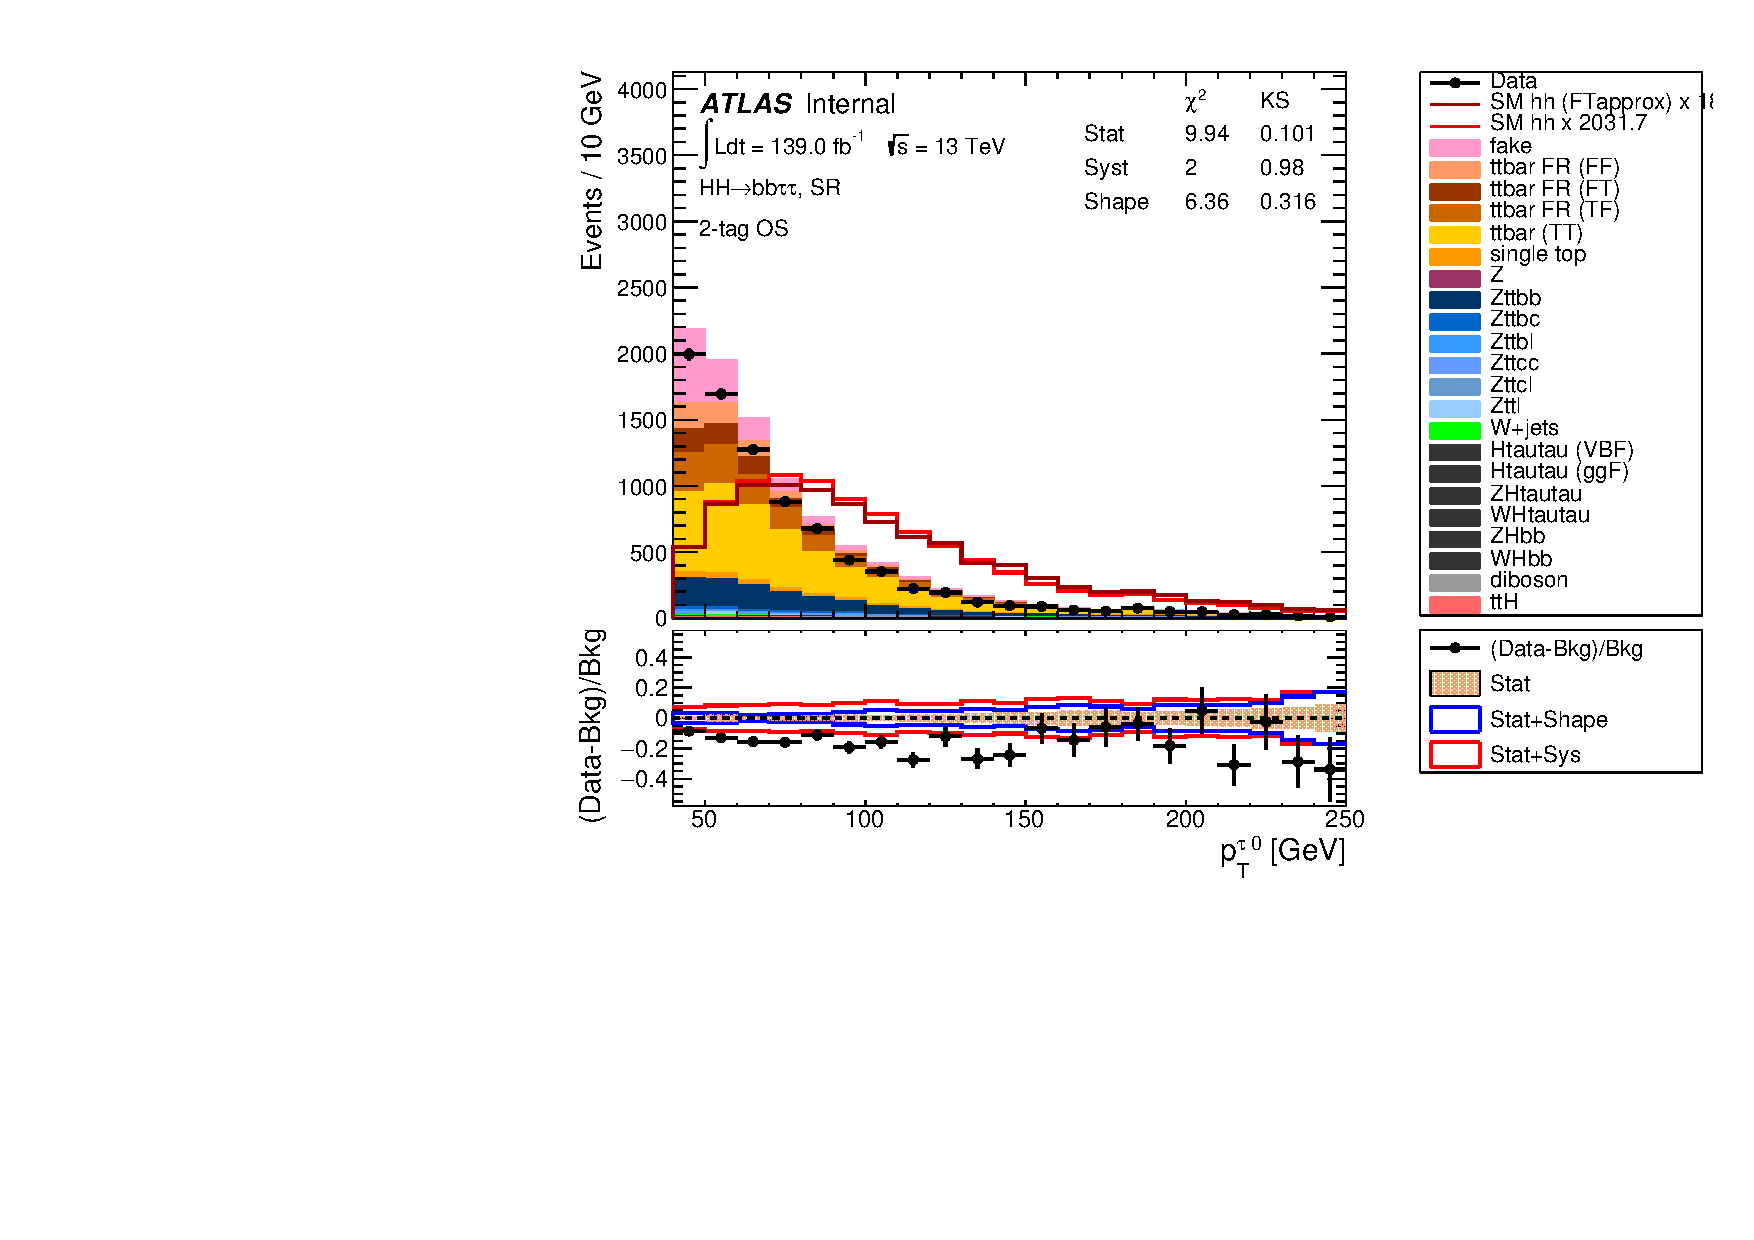
\includegraphics[width=.45\textwidth]{figures/selection/HadHad_HH/C_2tag2pjet_0ptv_LL_OS_Tau0Pt.pdf}}\quad
%\subfloat[]
%   {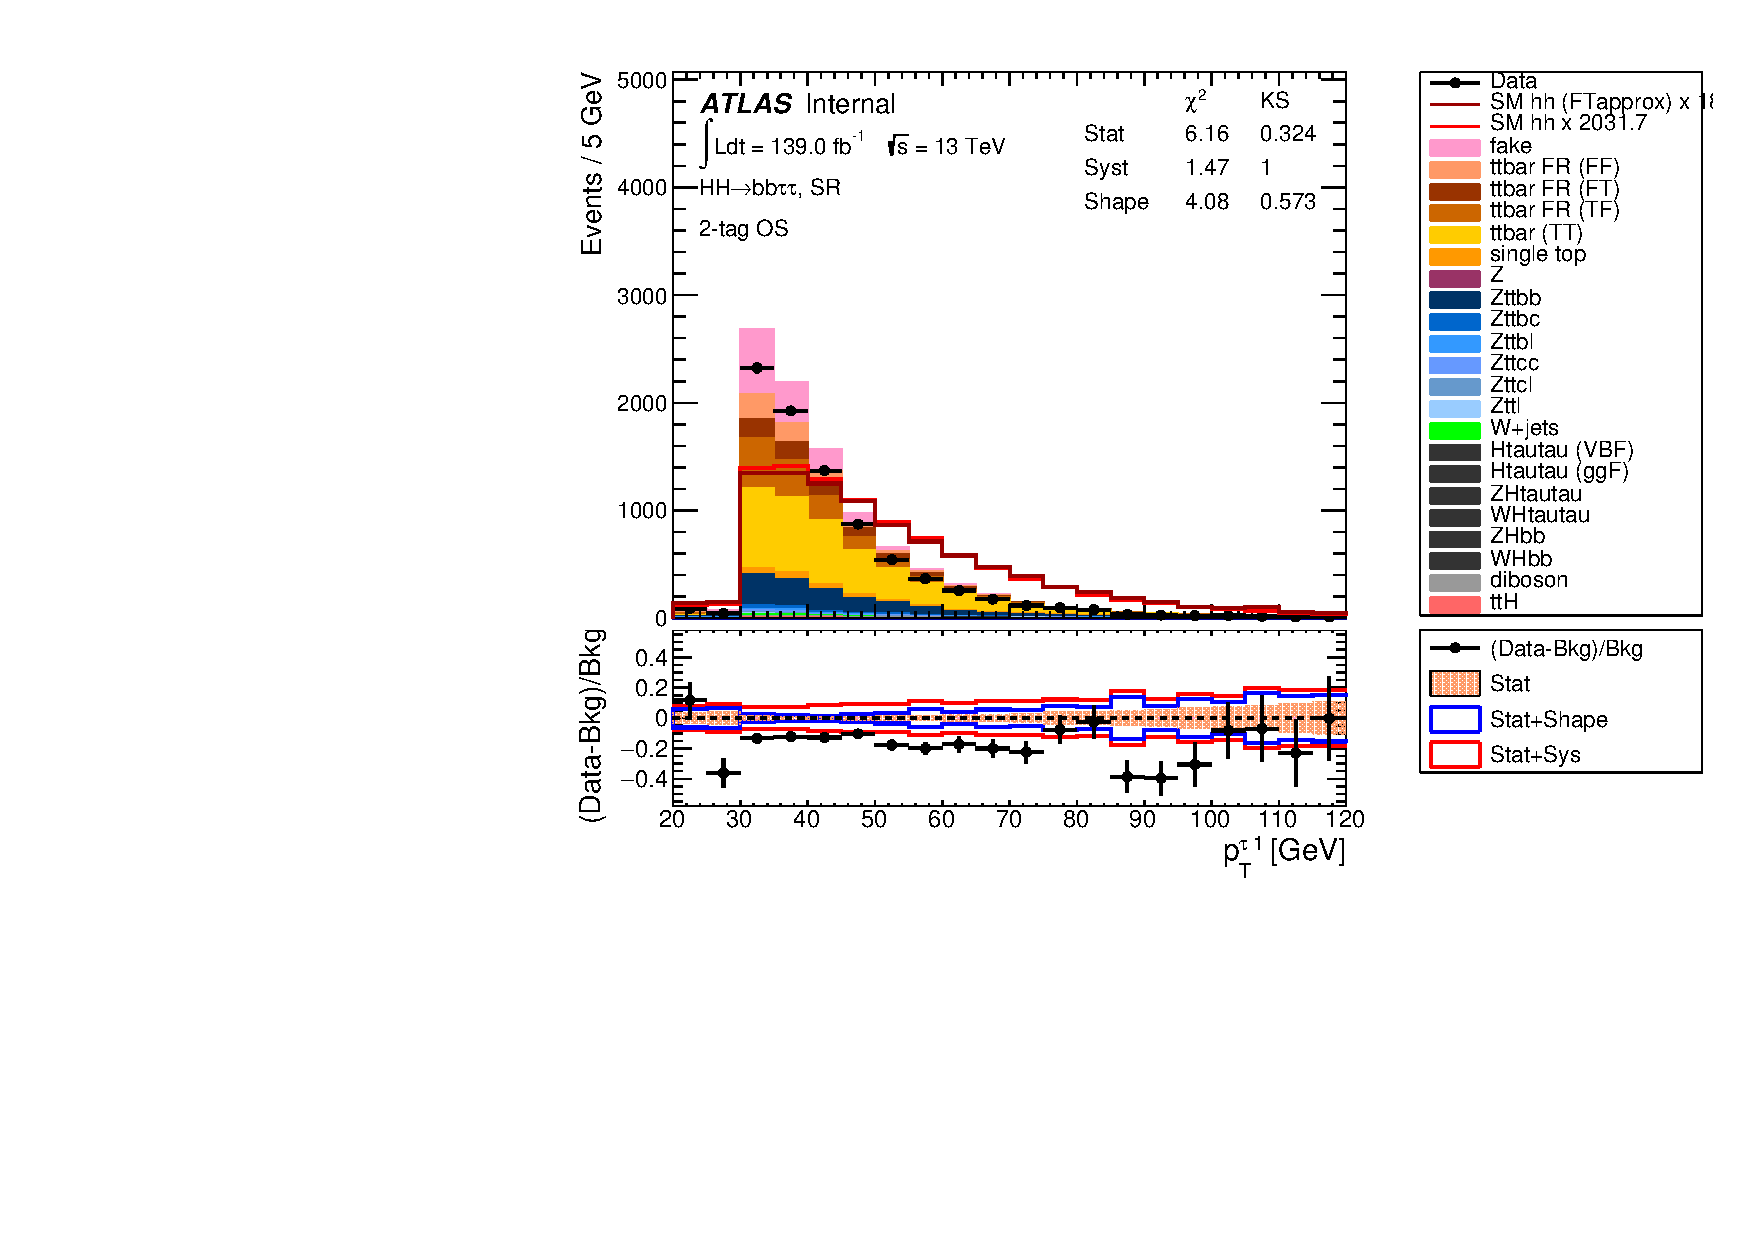
\includegraphics[width=.45\textwidth]{figures/selection/HadHad_HH/C_2tag2pjet_0ptv_LL_OS_Tau1Pt.pdf}} \quad
%\subfloat[]
%   {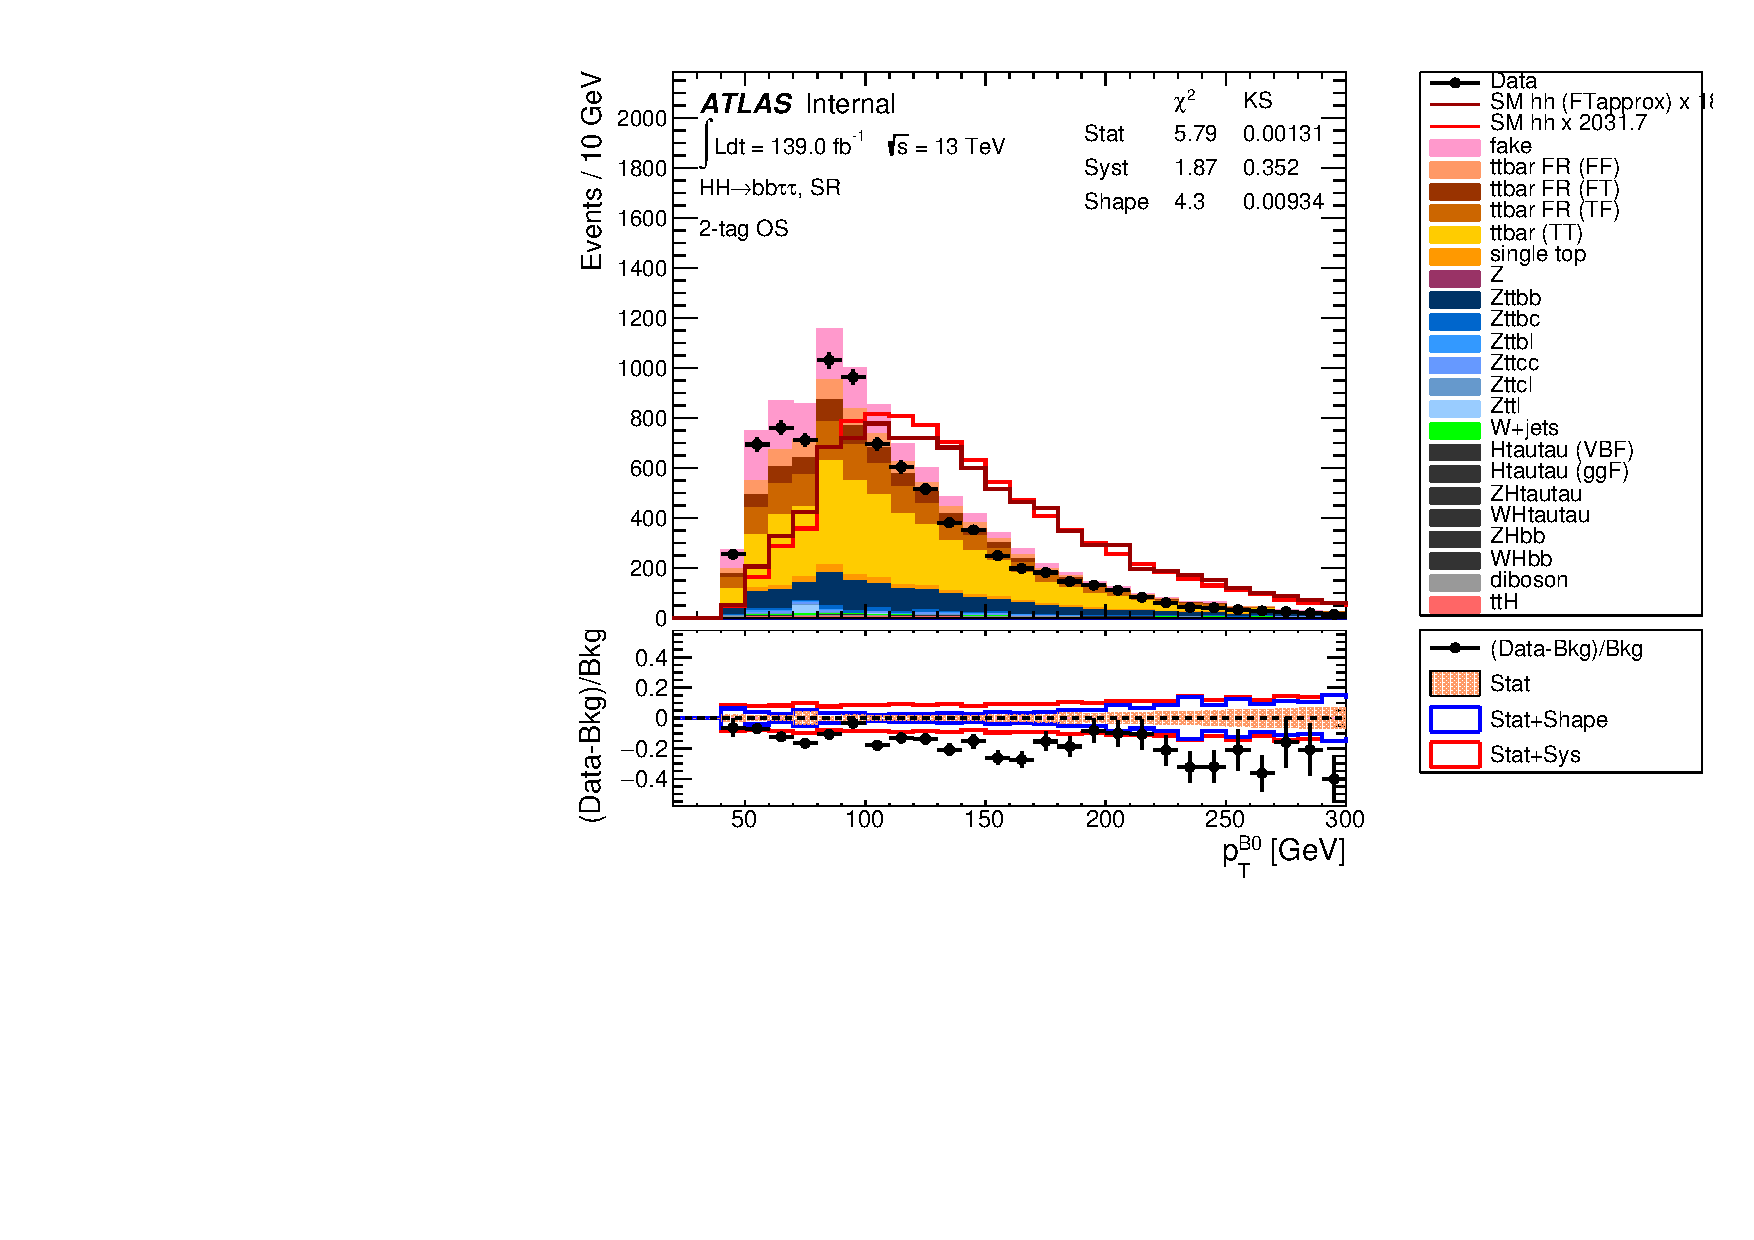
\includegraphics[width=.45\textwidth]{figures/selection/HadHad_HH/C_2tag2pjet_0ptv_LL_OS_pTB0.pdf}}\quad
%\subfloat[]
%   {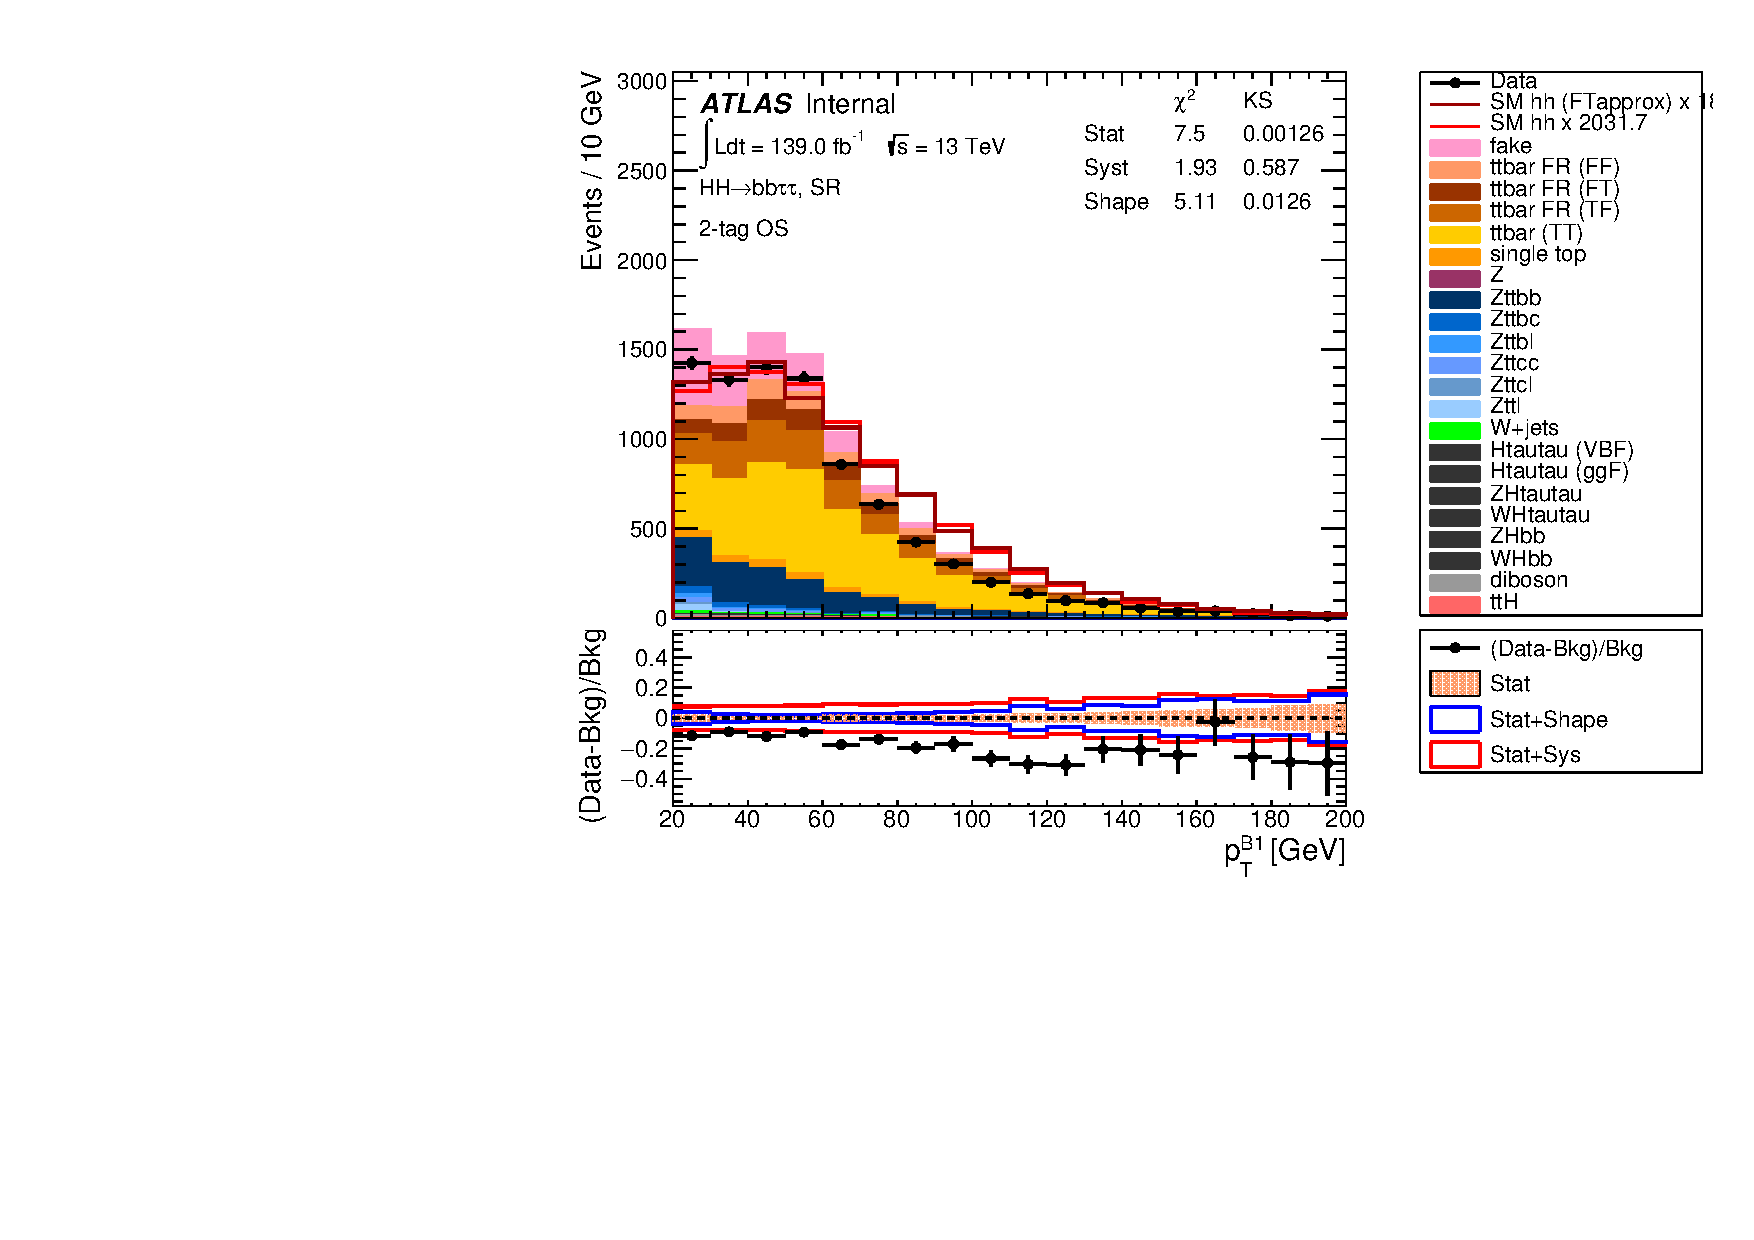
\includegraphics[width=.45\textwidth]{figures/selection/HadHad_HH/C_2tag2pjet_0ptv_LL_OS_pTB1.pdf}} \quad
%\caption{Leading and sub-leading $\tau_{had}$ and $b$-jet pre-fit \pt
%  distributions in the di-Higgs $bb\tau_{had}\tau_{had}$ signal region. The yields for Zttbb, Zttbc and Zttcc are scaled by 1.3. The uncertainty band includes CP uncertainties and $t\bar{t}$ and fake-$\tau_{had}$ backgrounds modelling uncertainties. (Inputs from 2020\_10\_16) (\textcolor{red}{To do: replace with plots from WSMaker including all uncertainties})}
%\label{fig:HadHadPreselectionPtDistributions}
%\end{figure}

\begin{figure}
\centering
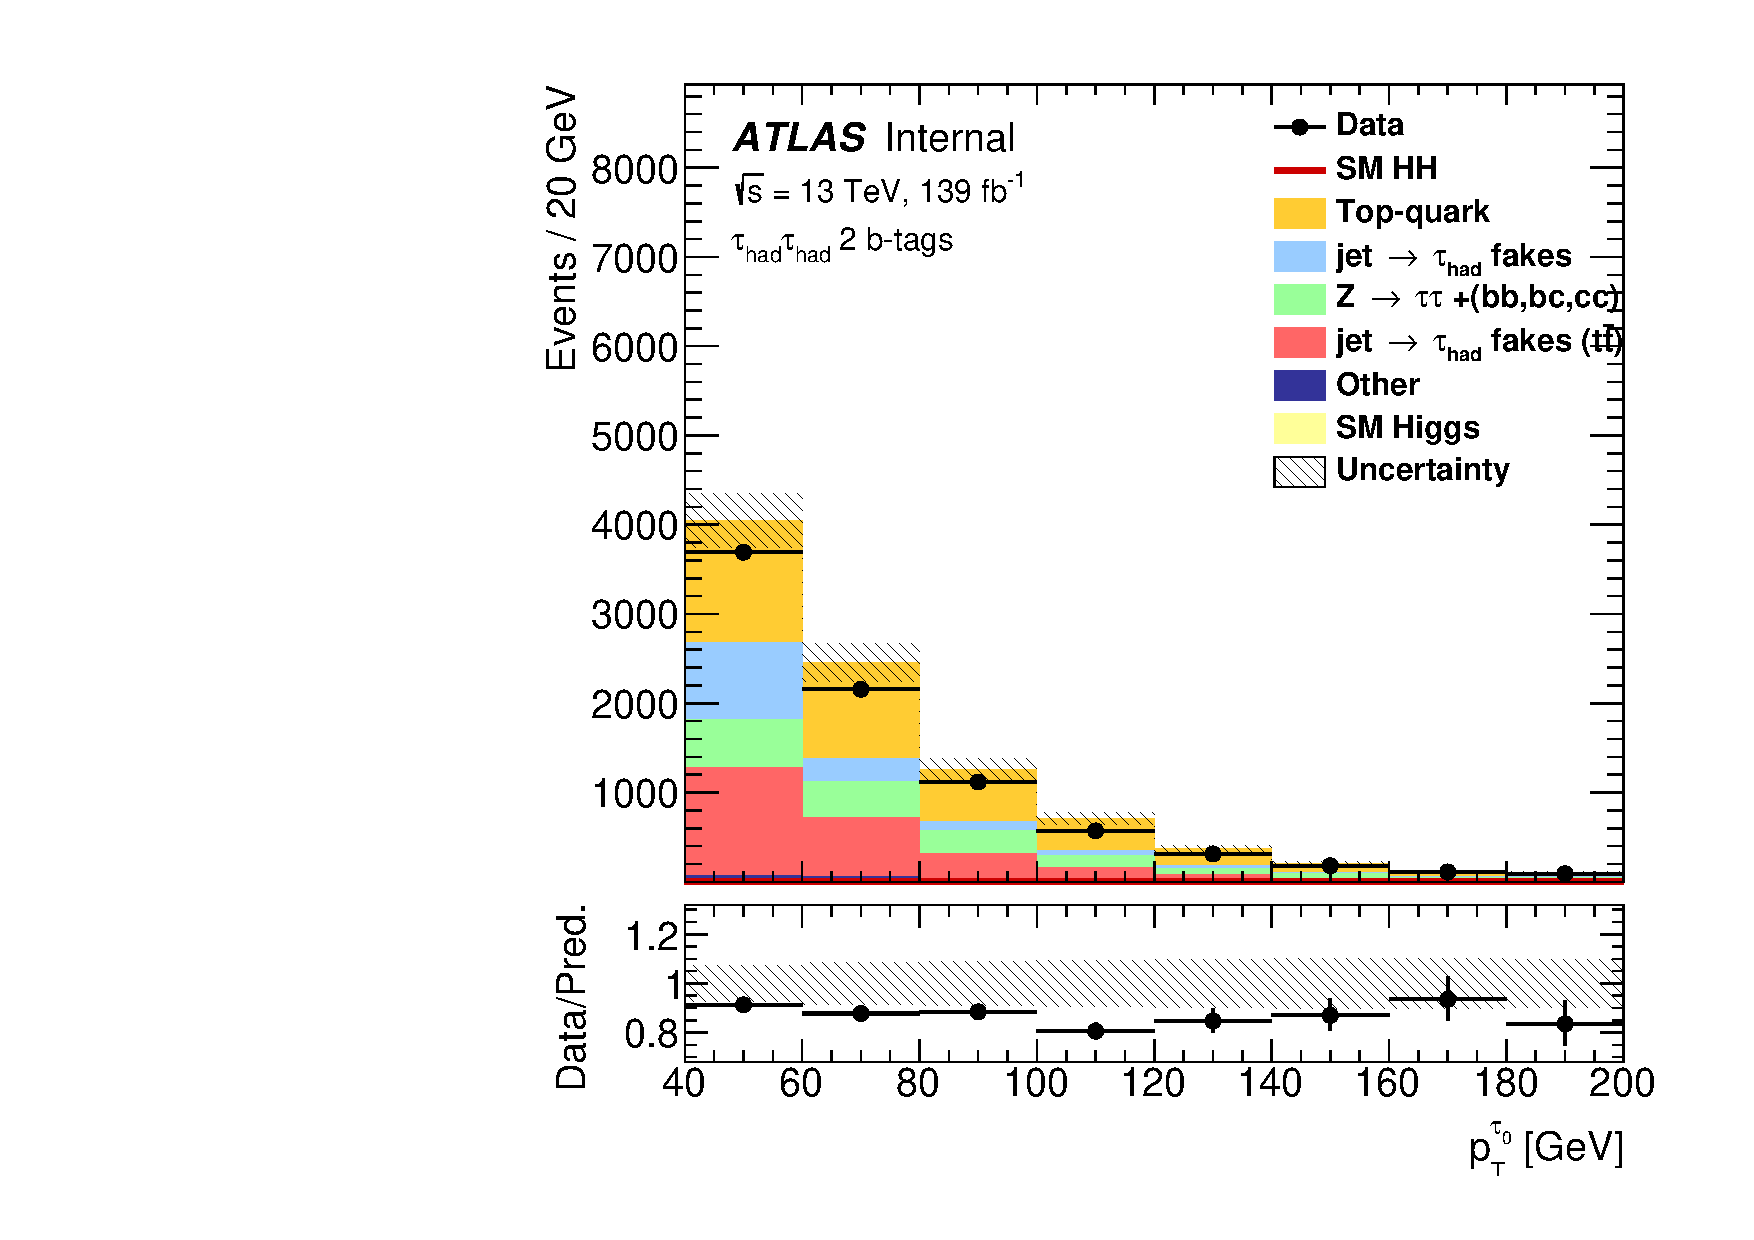
\includegraphics[width=.45\textwidth]{figures/selection/HadHad_HH/Region_BMin0_incJet1_distTau0Pt_J2_Y2015_DLLOS_T2_SpcTauHH_L0_Prefit.pdf}
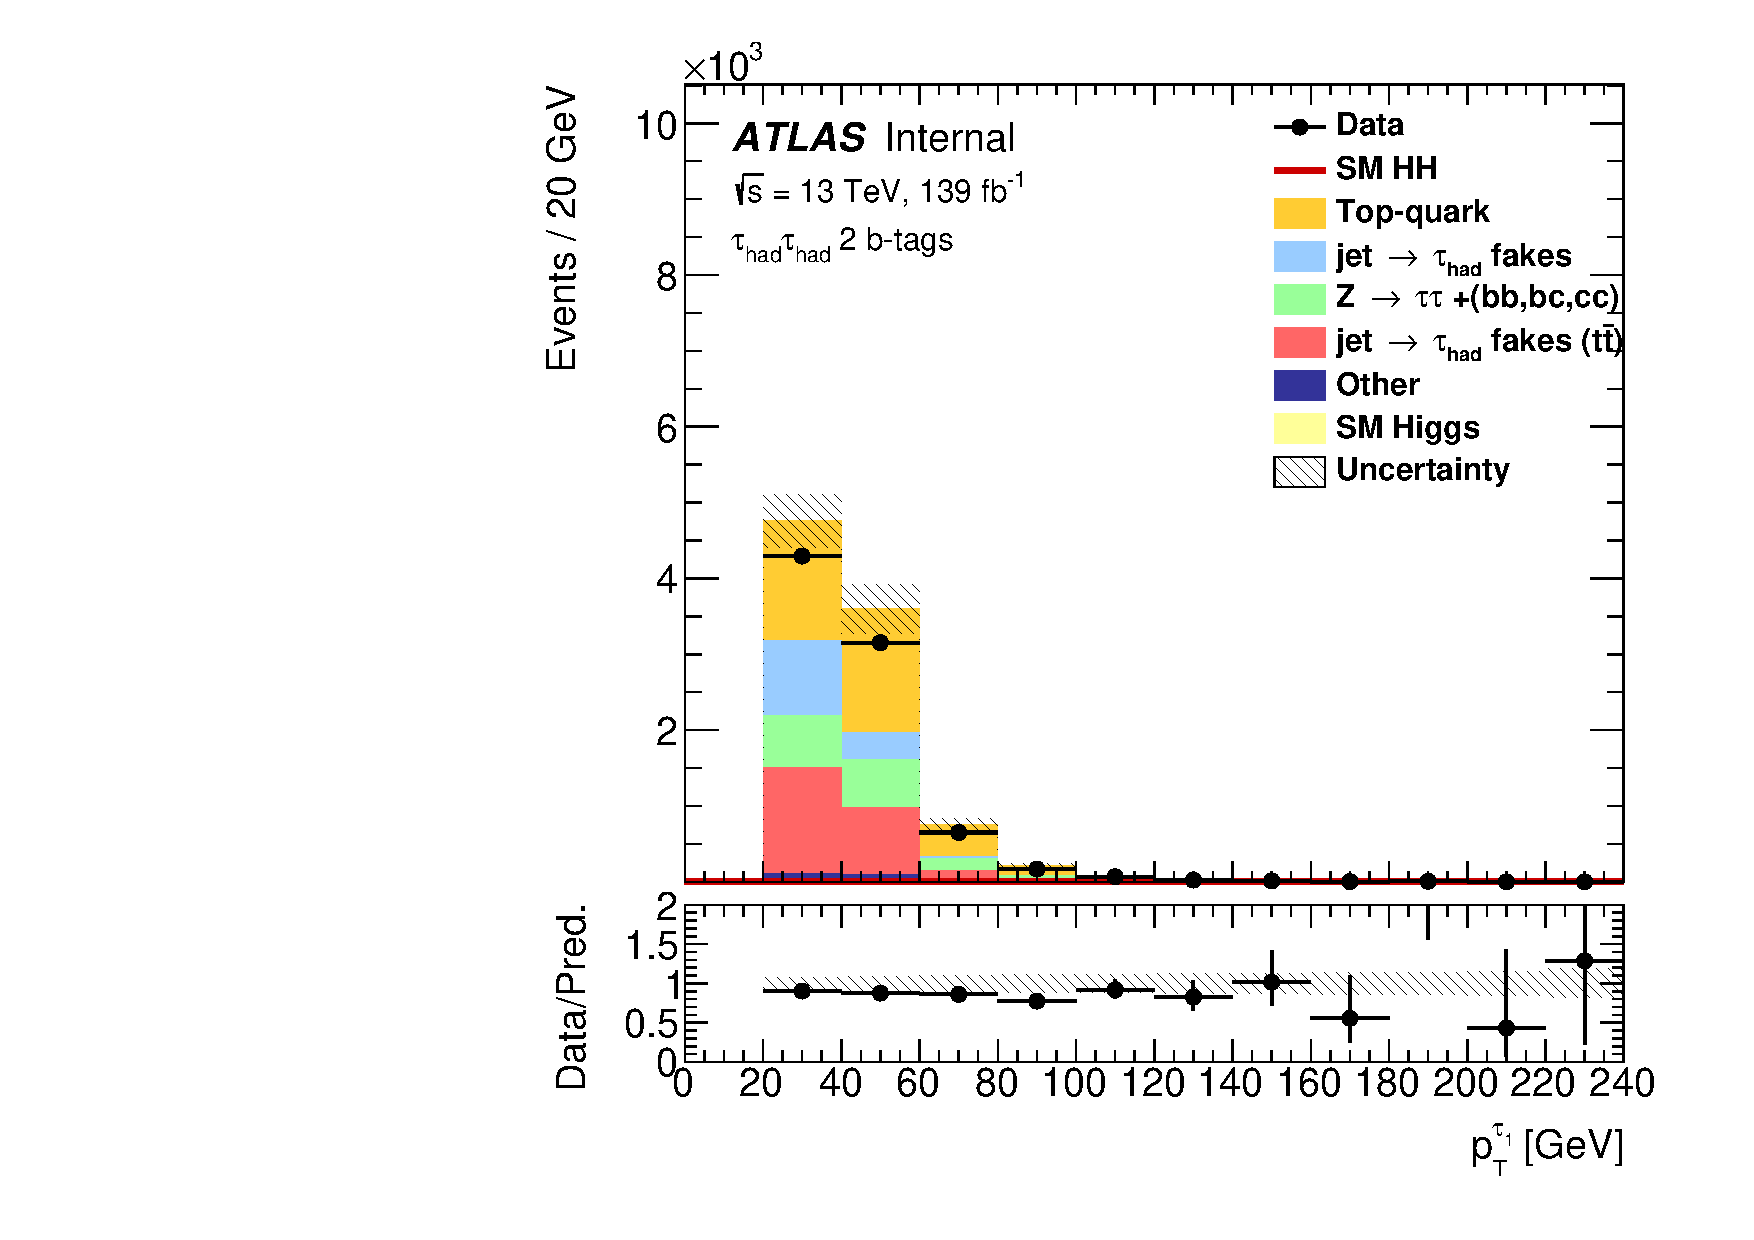
\includegraphics[width=.45\textwidth]{figures/selection/HadHad_HH/Region_BMin0_incJet1_distTau1Pt_J2_Y2015_DLLOS_T2_SpcTauHH_L0_Prefit.pdf}\\
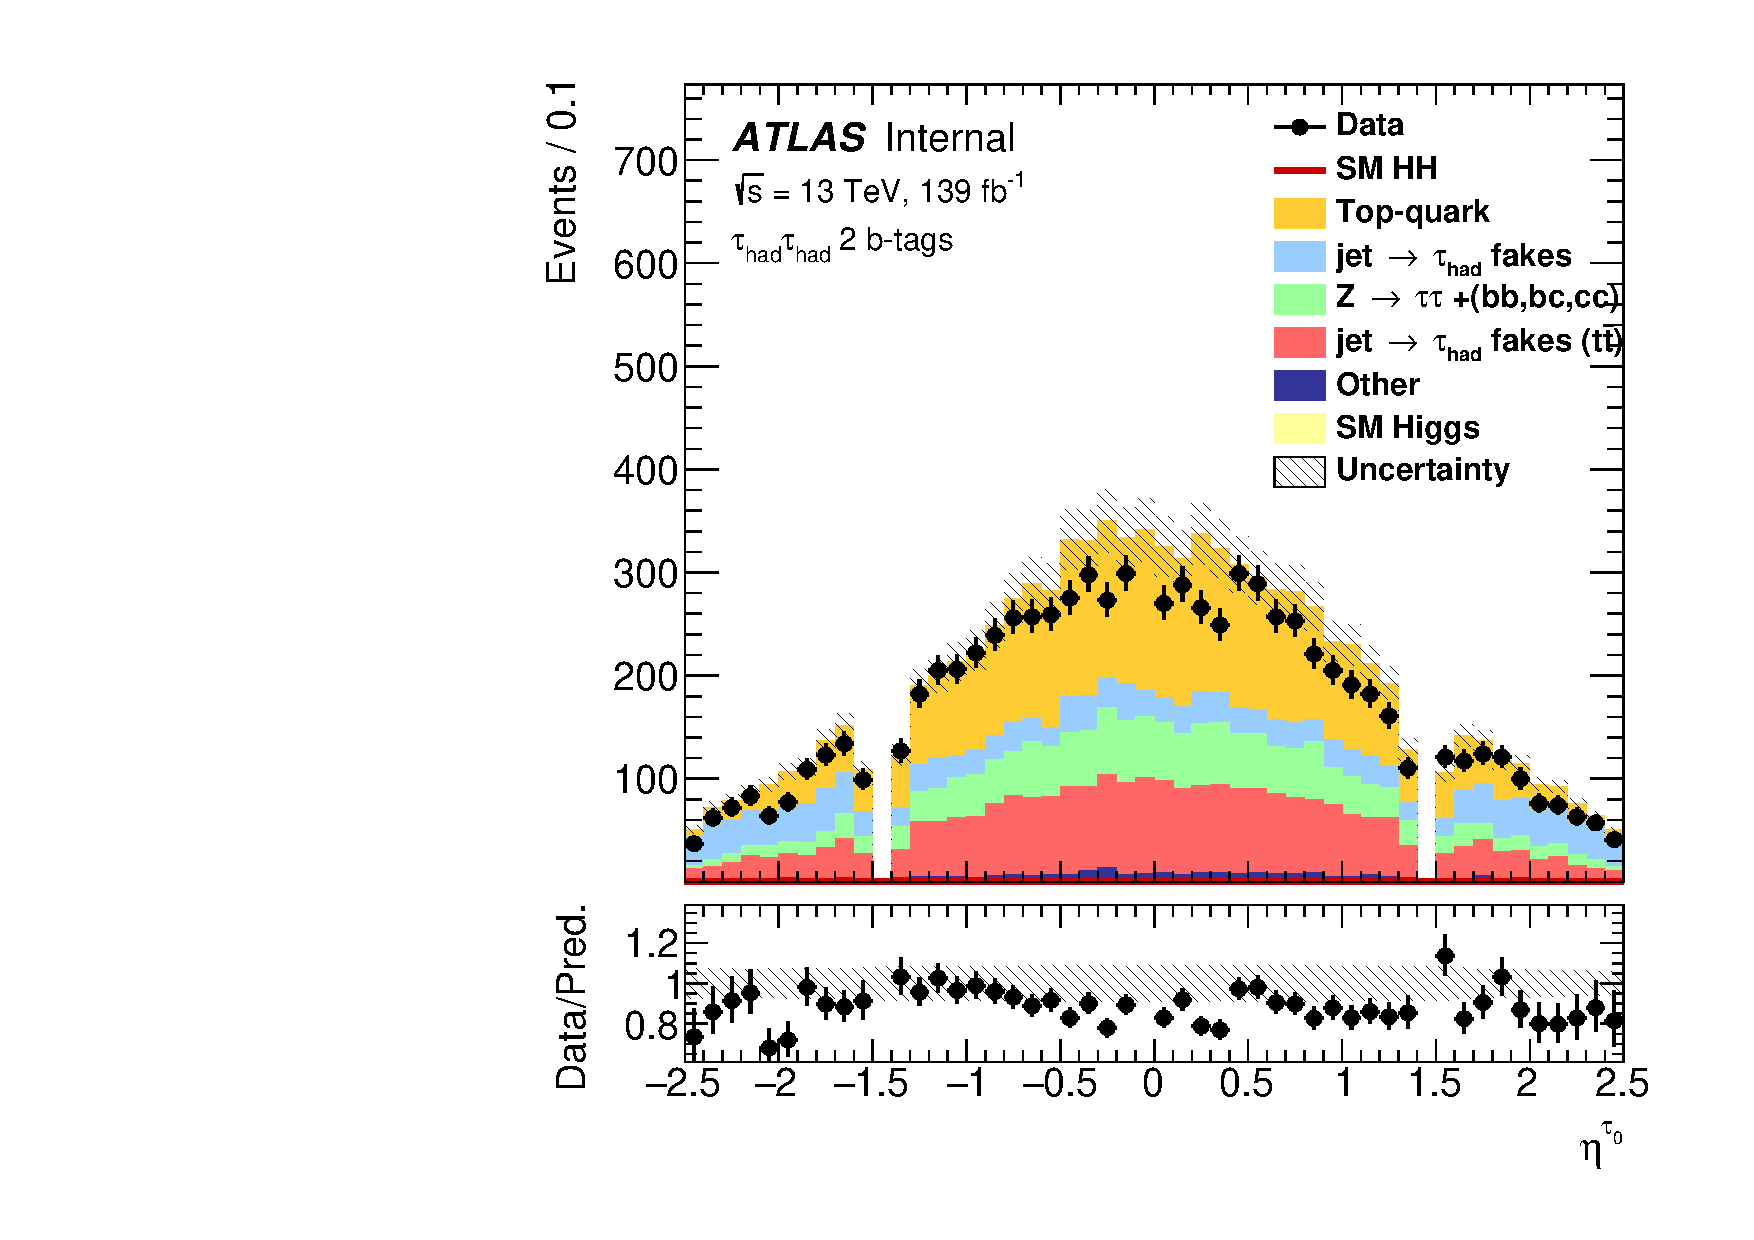
\includegraphics[width=.45\textwidth]{figures/selection/HadHad_HH/Region_BMin0_incJet1_distTau0Eta_J2_Y2015_DLLOS_T2_SpcTauHH_L0_Prefit.pdf}
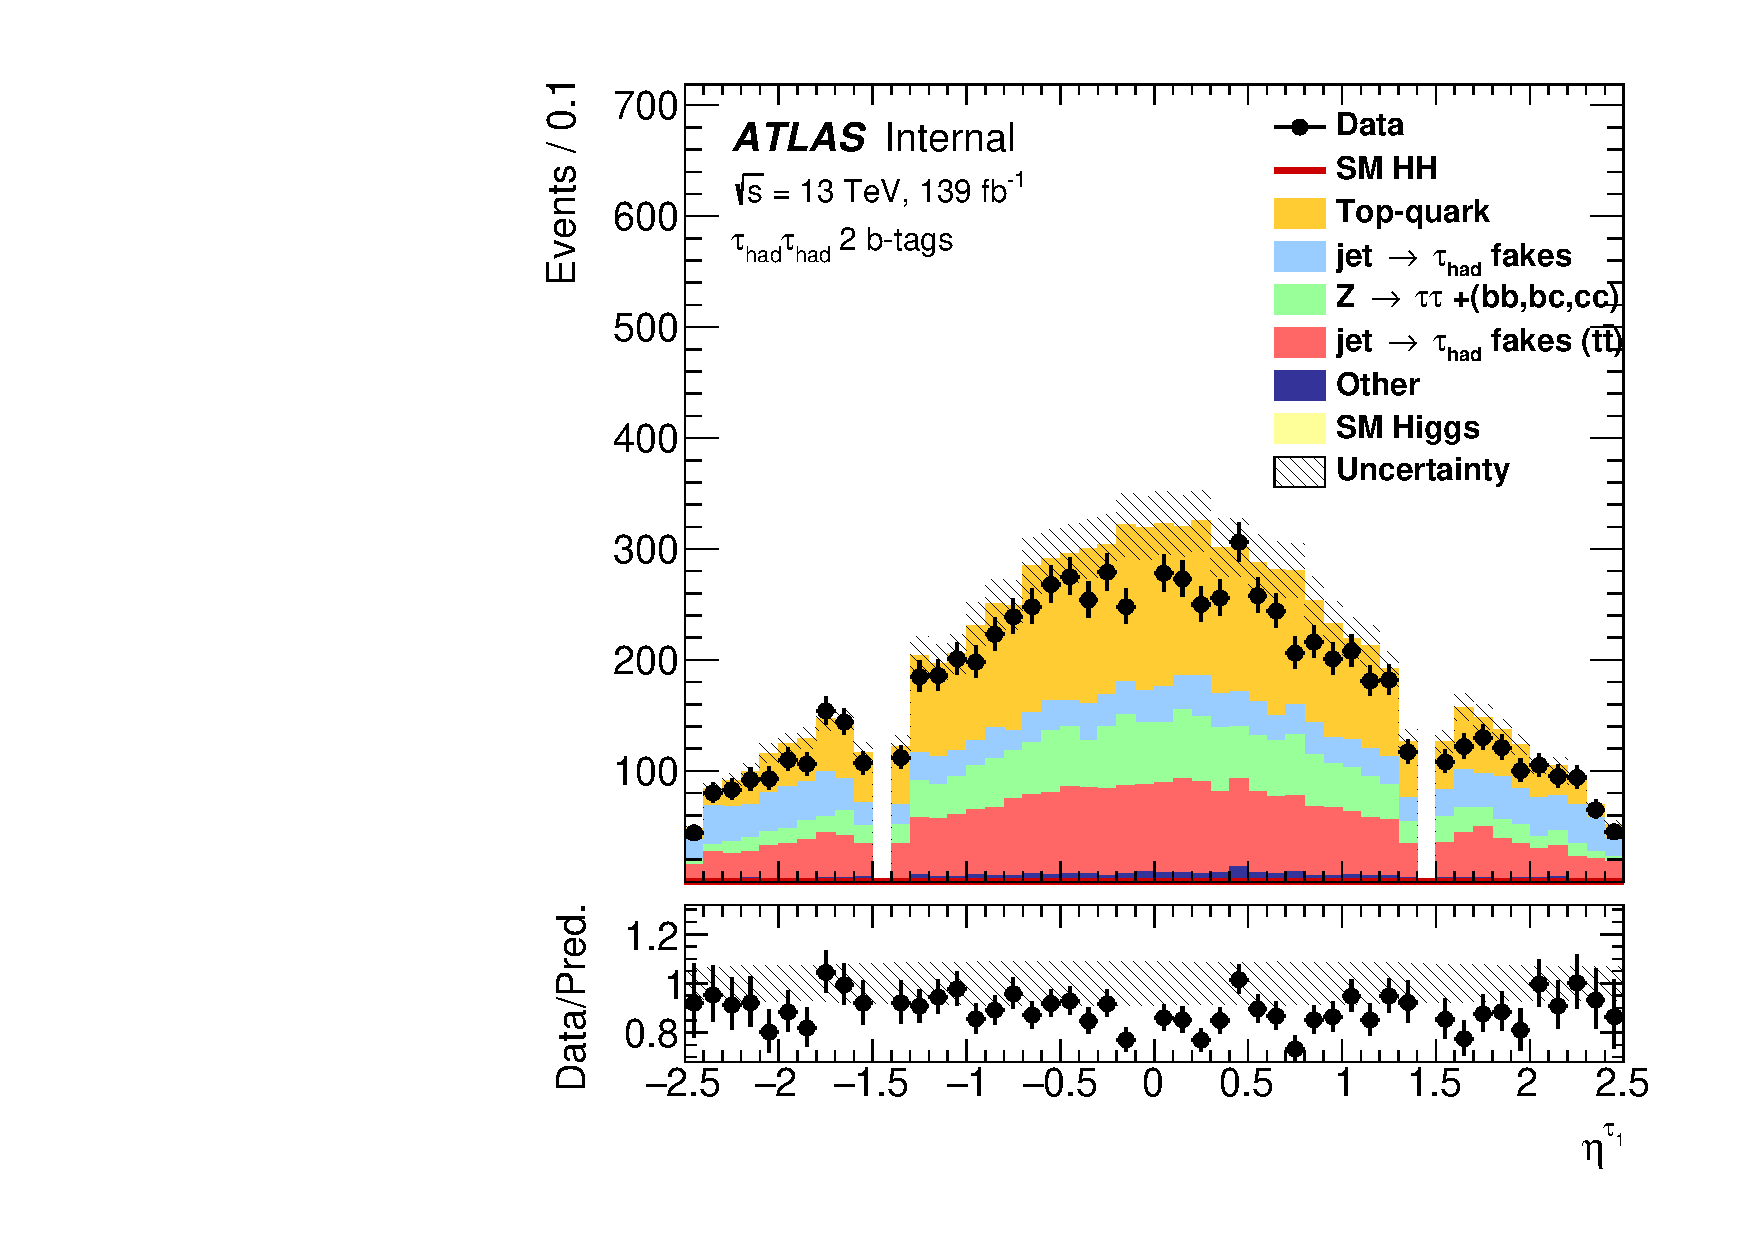
\includegraphics[width=.45\textwidth]{figures/selection/HadHad_HH/Region_BMin0_incJet1_distTau1Eta_J2_Y2015_DLLOS_T2_SpcTauHH_L0_Prefit.pdf}\\
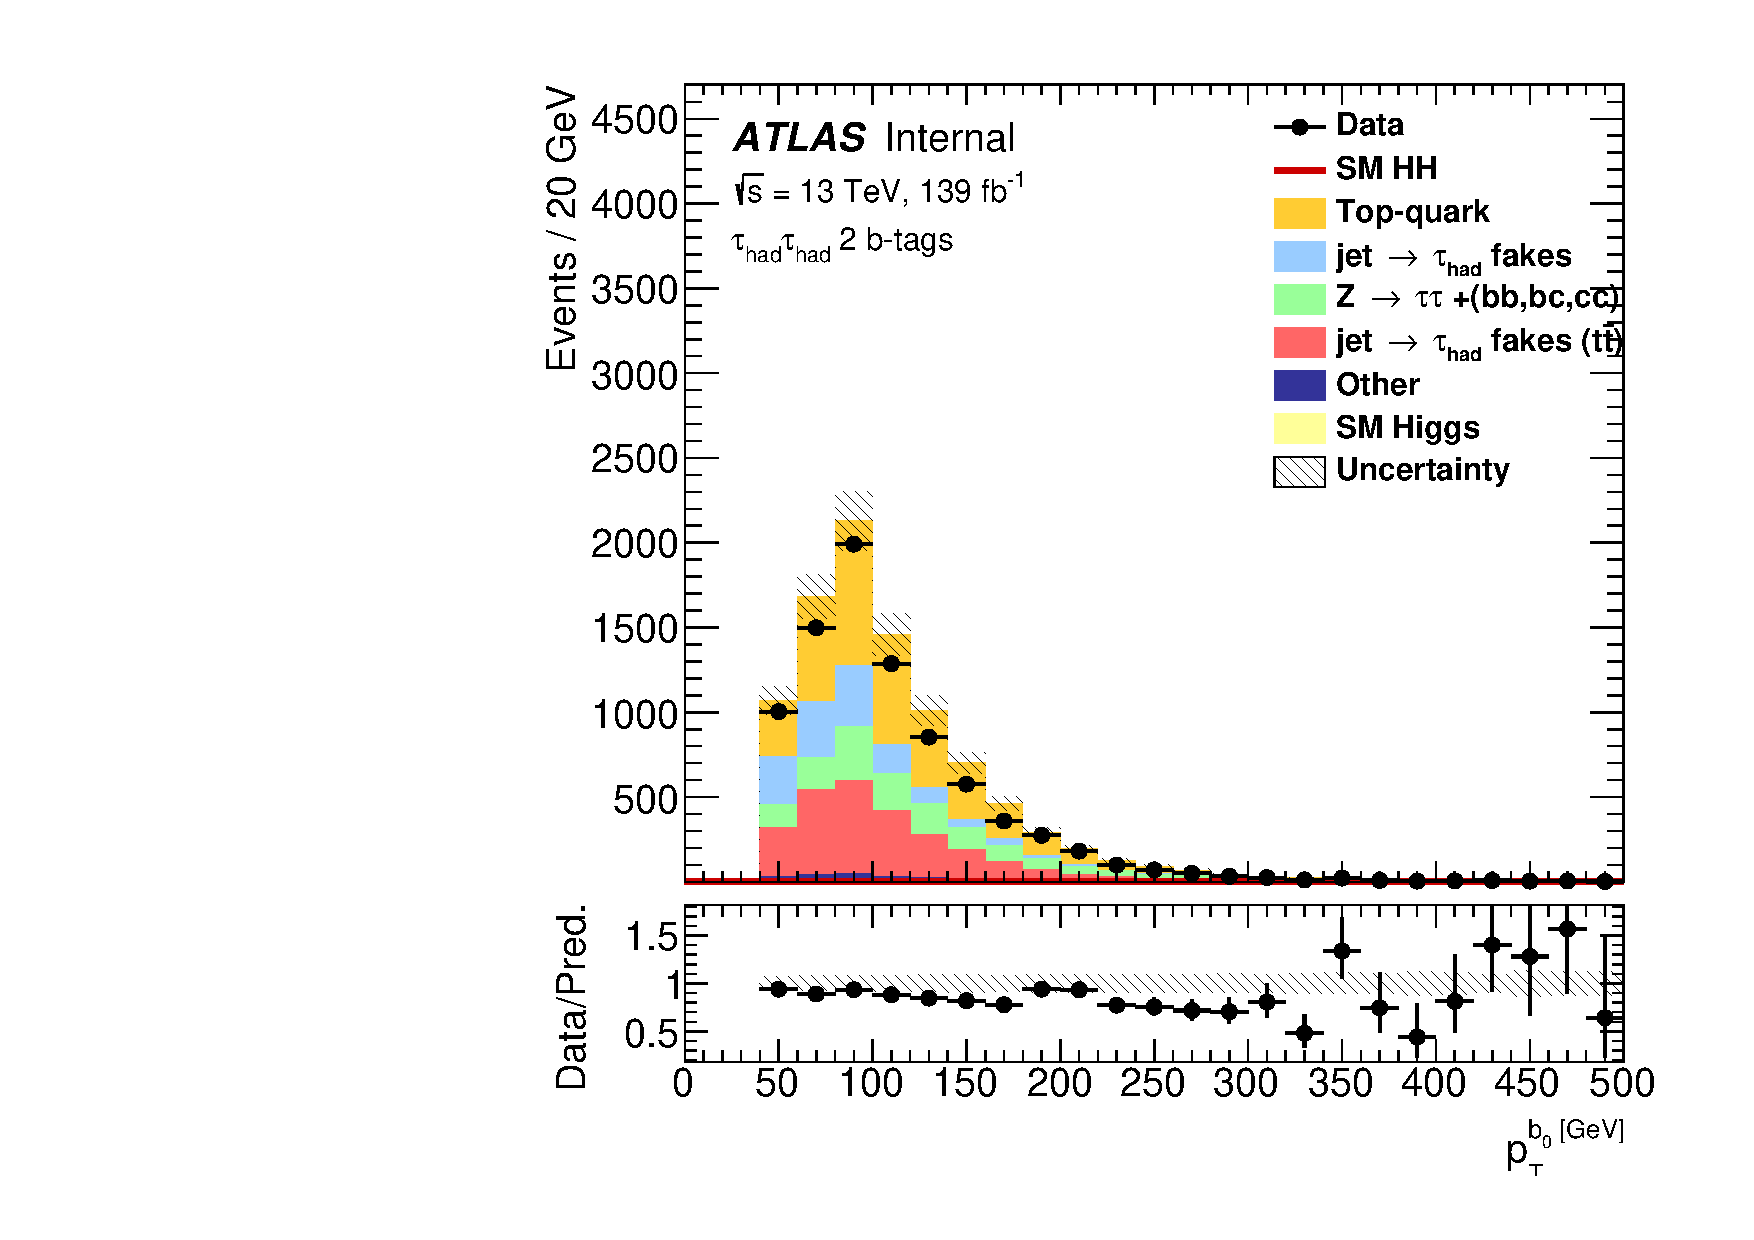
\includegraphics[width=.45\textwidth]{figures/selection/HadHad_HH/Region_BMin0_incJet1_distJet0Pt_J2_Y2015_DLLOS_T2_SpcTauHH_L0_Prefit.pdf}
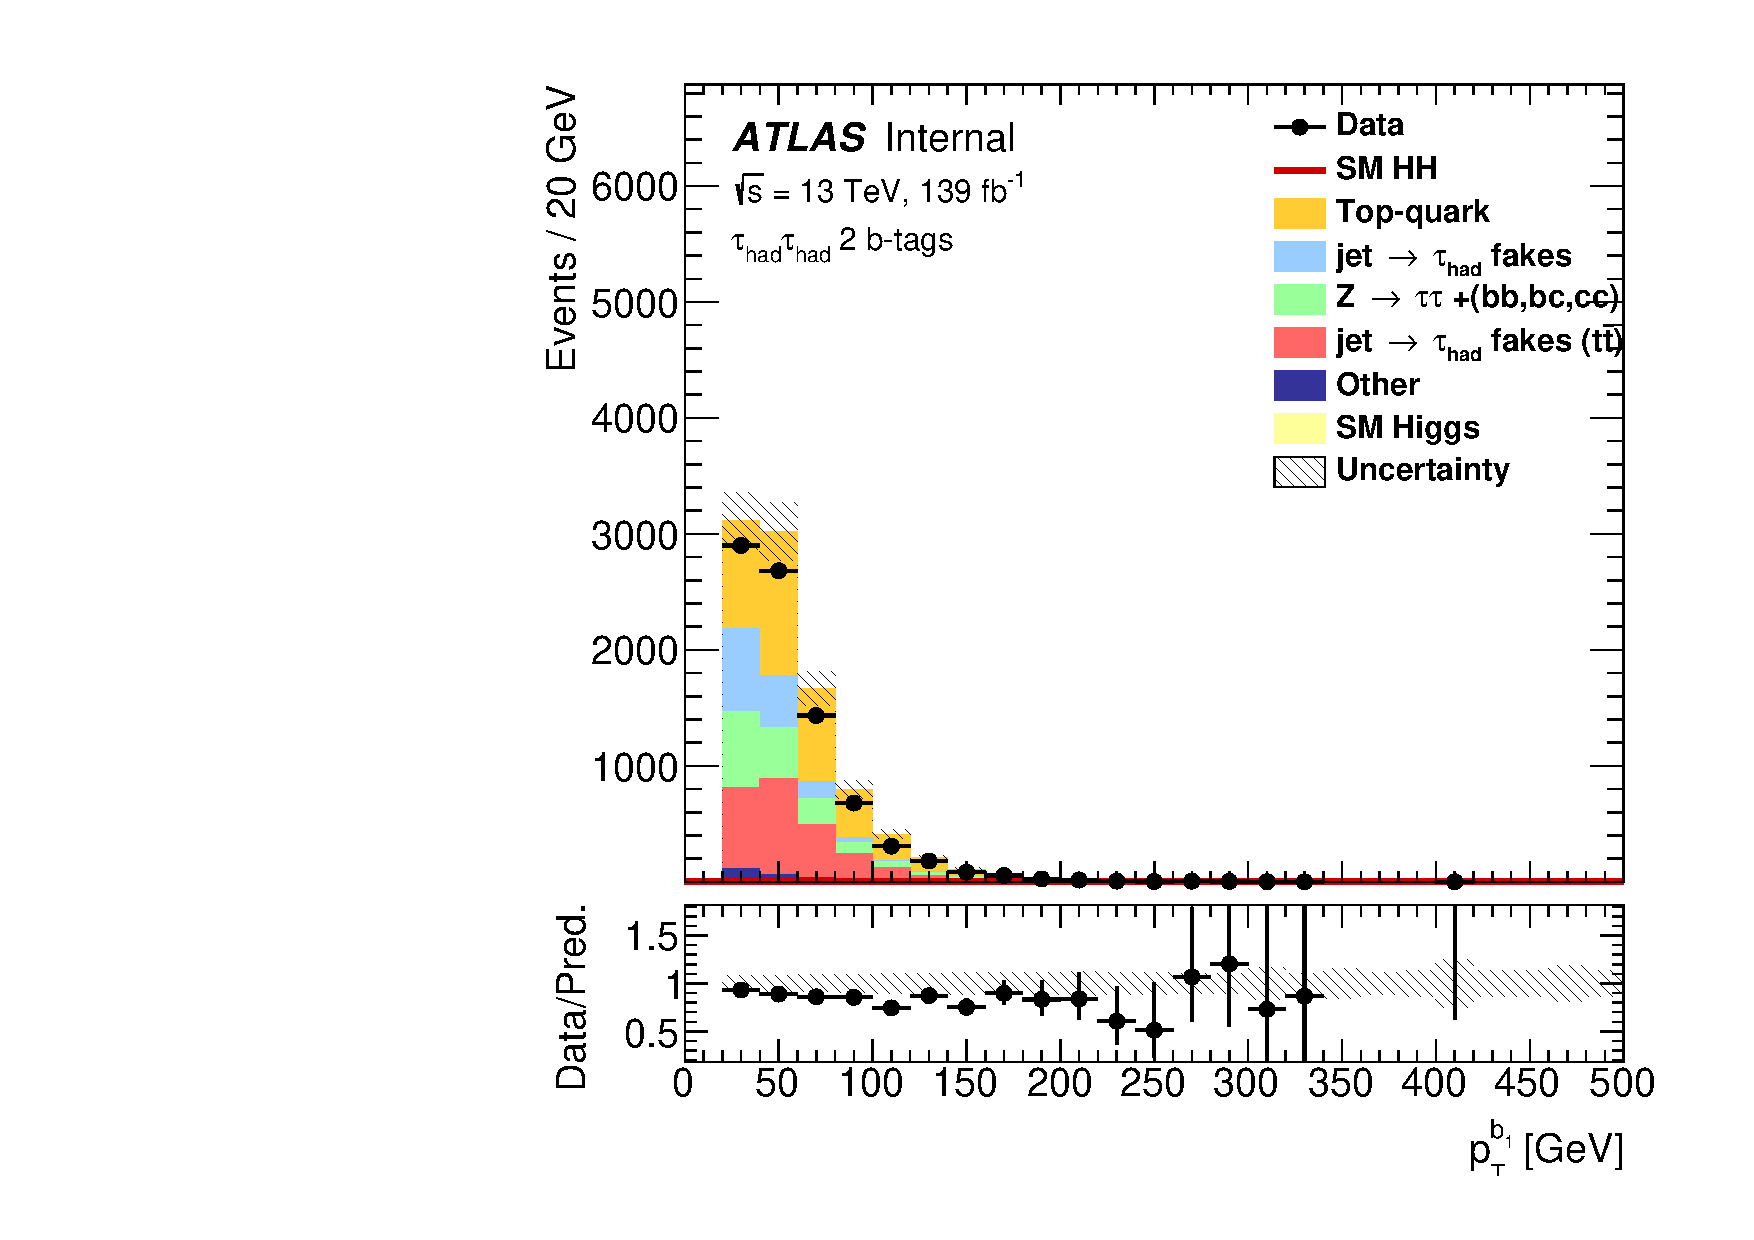
\includegraphics[width=.45\textwidth]{figures/selection/HadHad_HH/Region_BMin0_incJet1_distJet1Pt_J2_Y2015_DLLOS_T2_SpcTauHH_L0_Prefit.pdf}
\caption{Leading and sub-leading $\tau_{had}$ \pt and $\eta$ and $b$-jet \pt pre-fit
  distributions in the di-Higgs \hadhad signal region. (Inputs from 2021\_01\_15)}
\label{fig:HadHadPreselectionPtDistributions}
\end{figure}

\begin{figure}
\centering
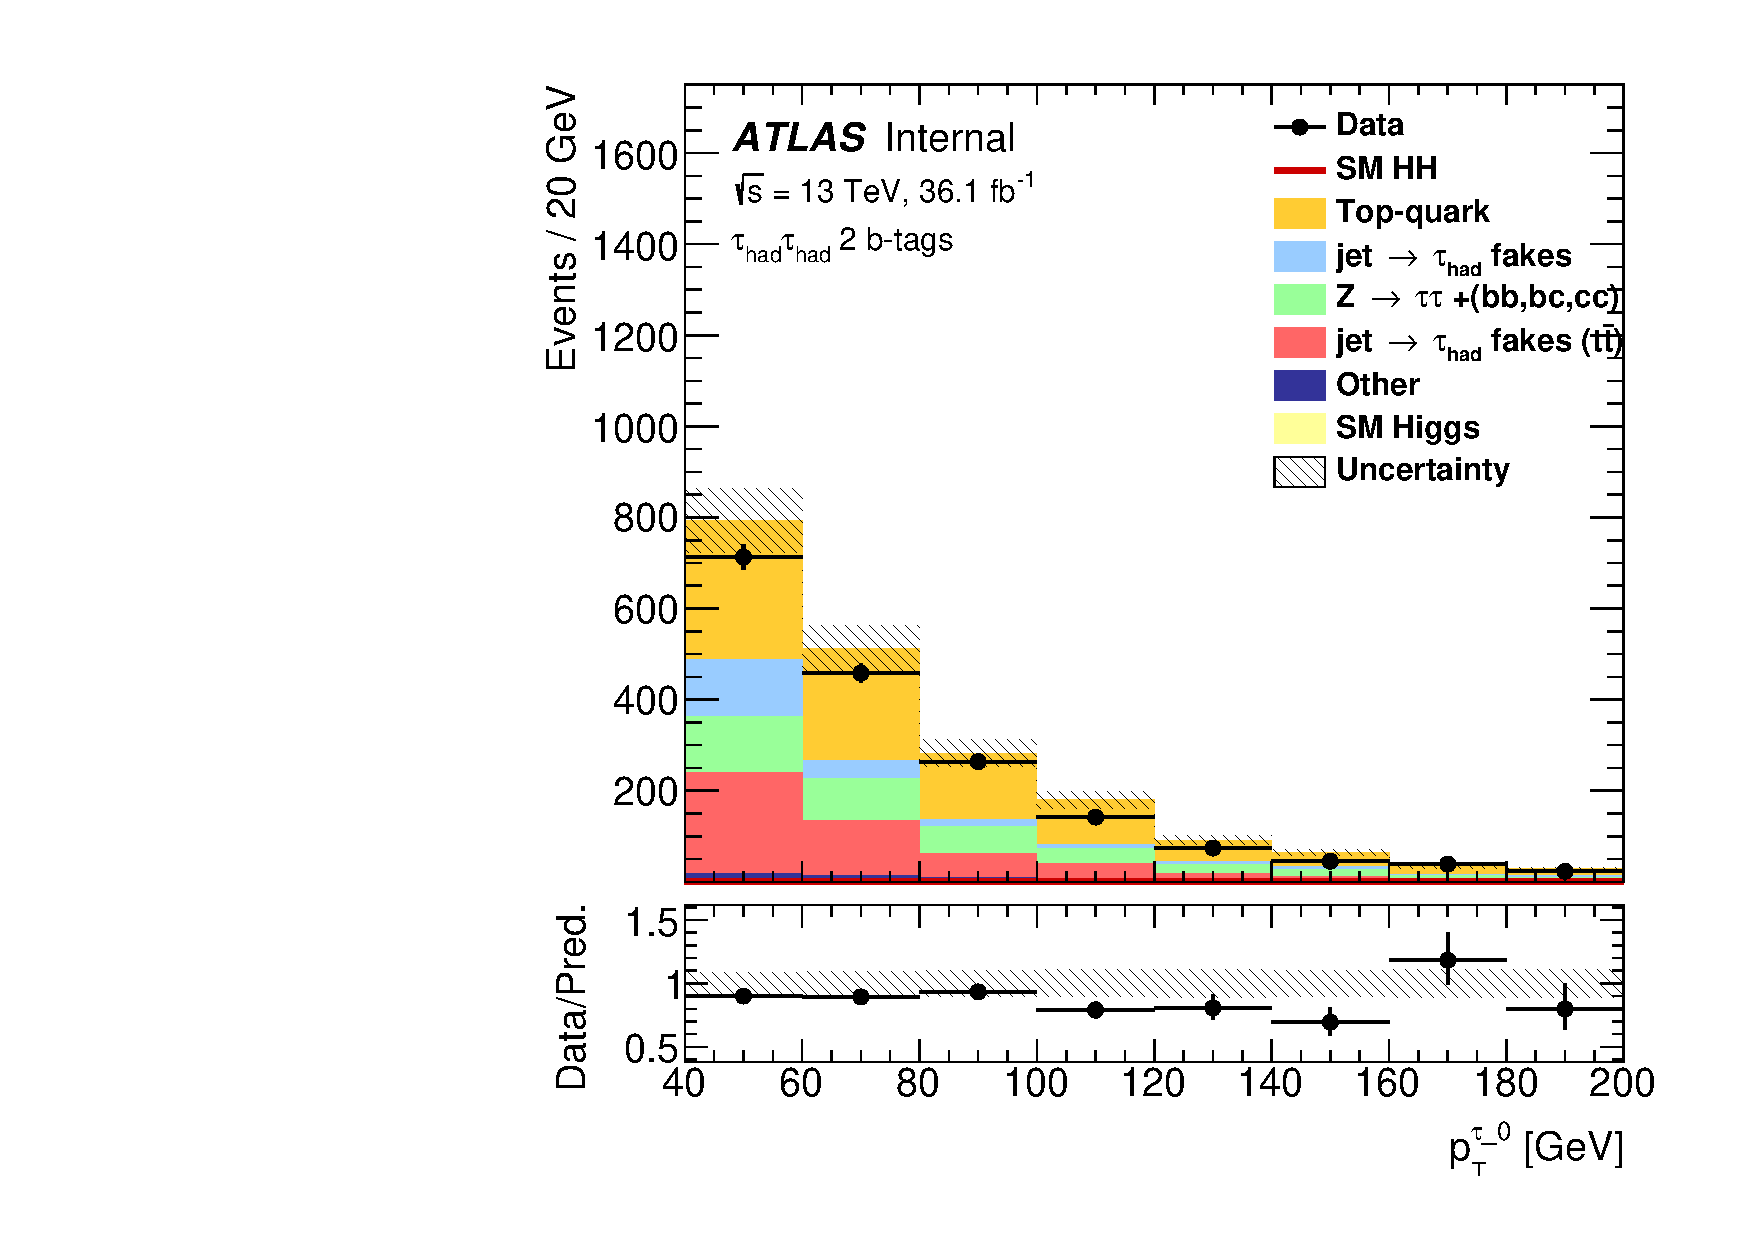
\includegraphics[width=.45\textwidth]{figures/selection/HadHad_HH/Plots2015/Region_BMin0_incJet1_distTau0Pt_J2_Y2015_DLLOS_T2_SpcTauHH_L0_Prefit.pdf}
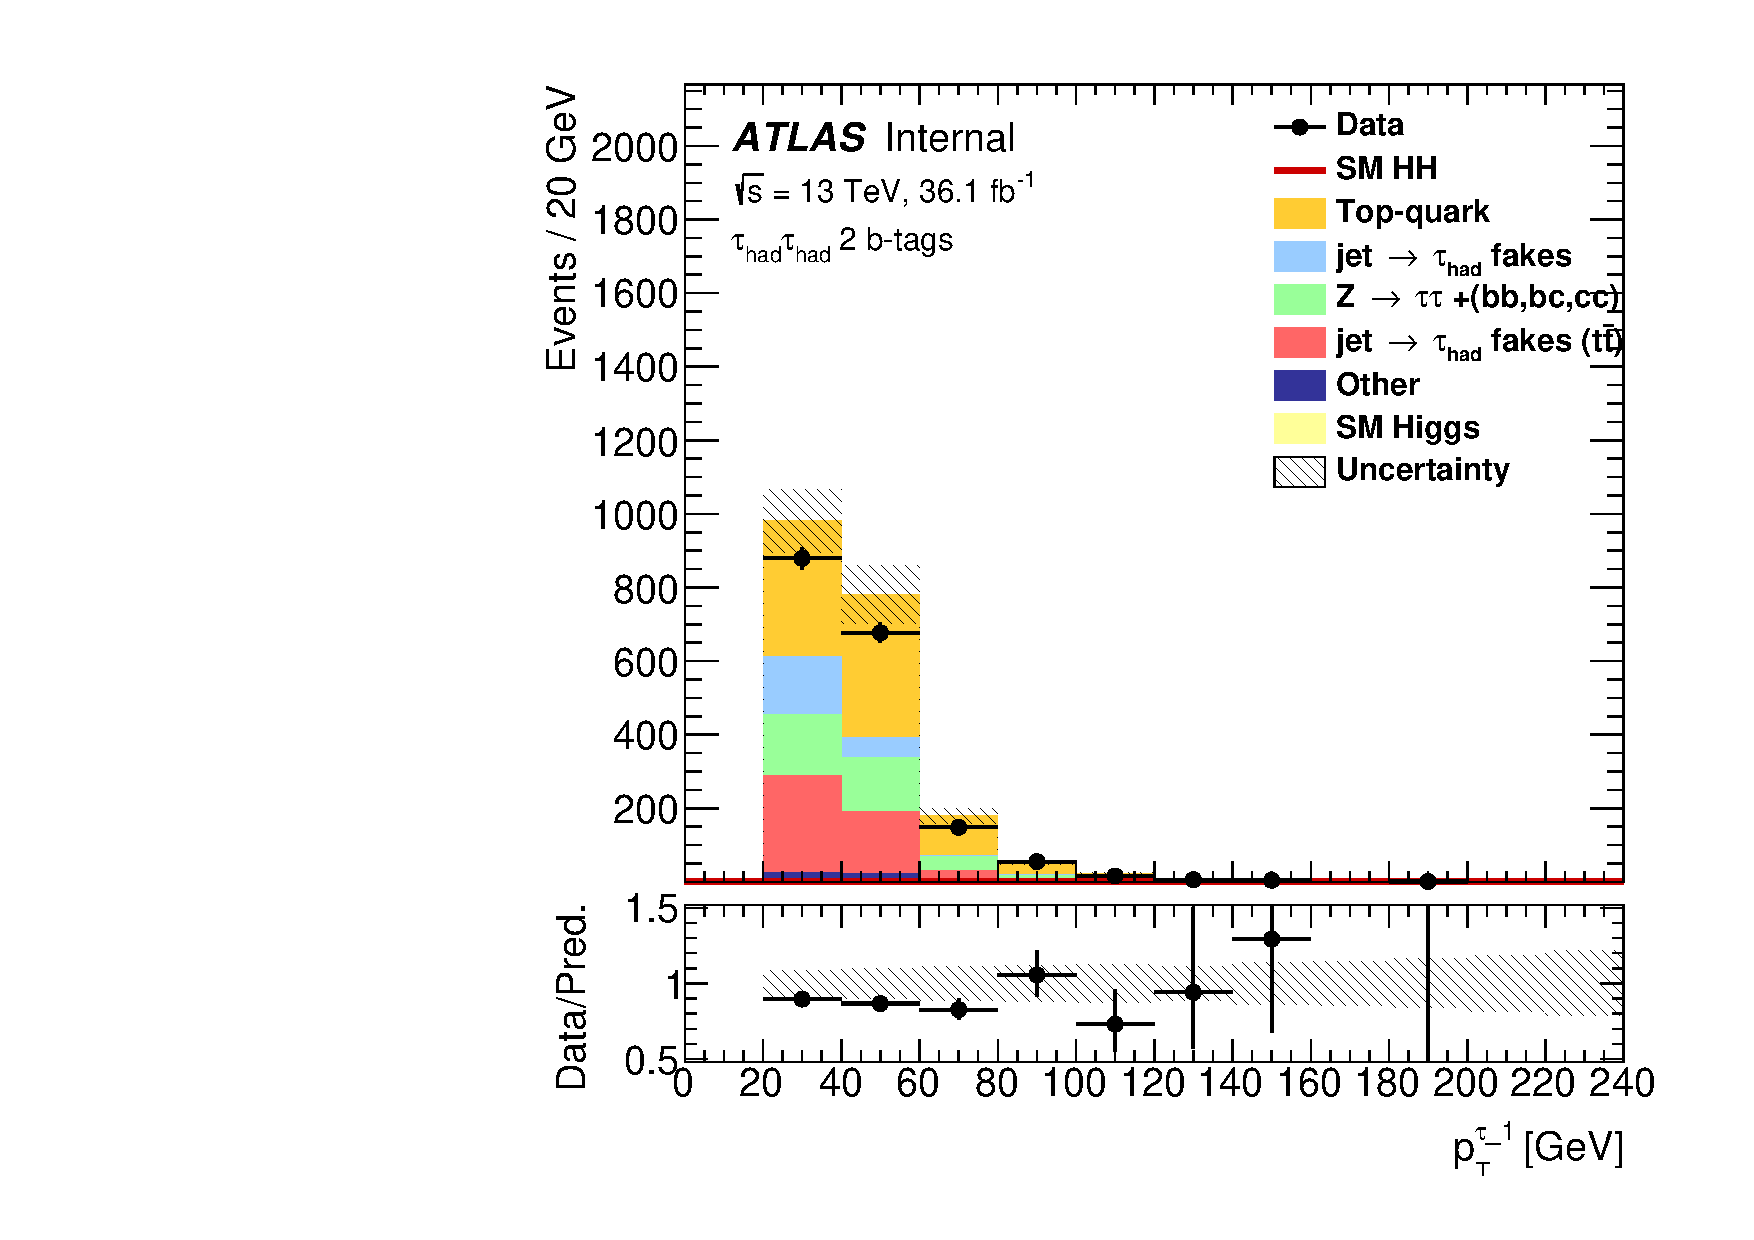
\includegraphics[width=.45\textwidth]{figures/selection/HadHad_HH/Plots2015/Region_BMin0_incJet1_distTau1Pt_J2_Y2015_DLLOS_T2_SpcTauHH_L0_Prefit.pdf}\\
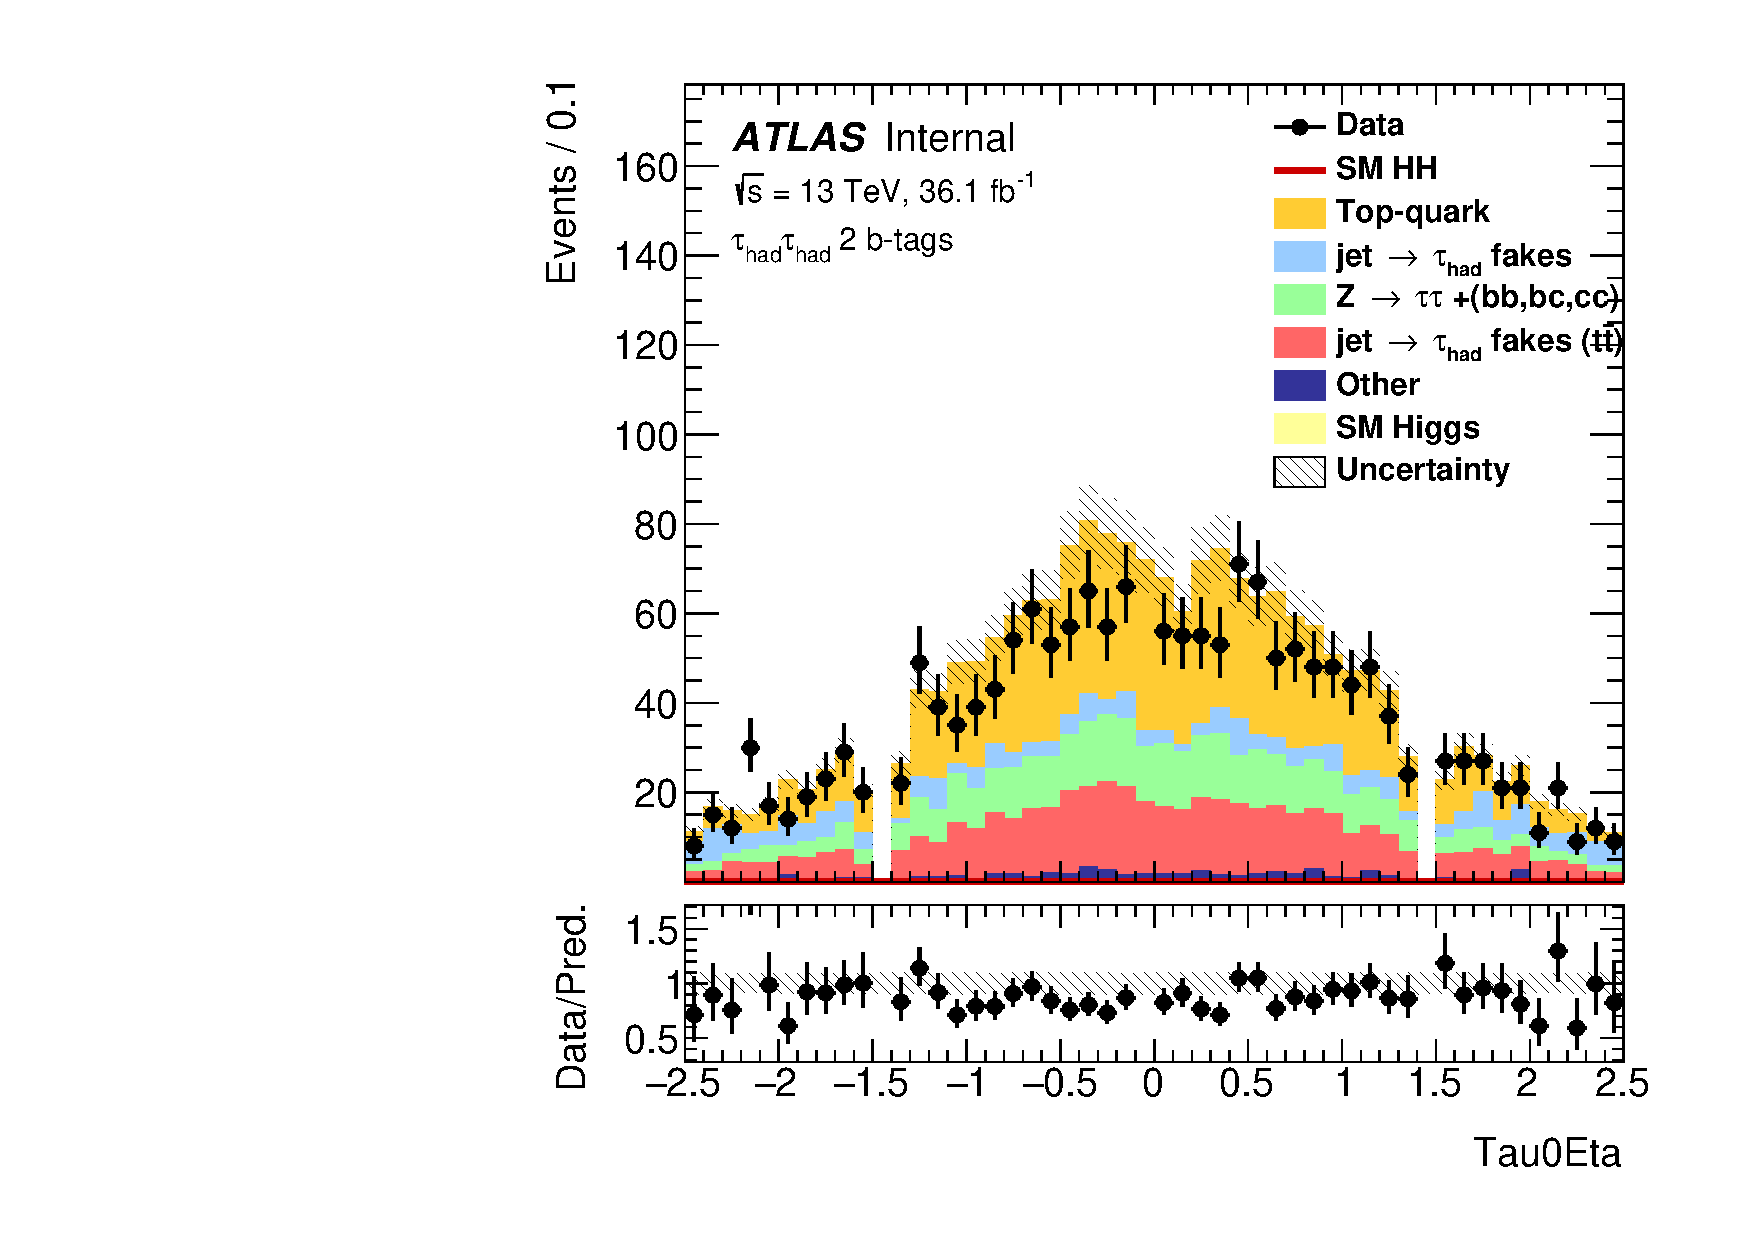
\includegraphics[width=.45\textwidth]{figures/selection/HadHad_HH/Plots2015/Region_BMin0_incJet1_distTau0Eta_J2_Y2015_DLLOS_T2_SpcTauHH_L0_Prefit.pdf}
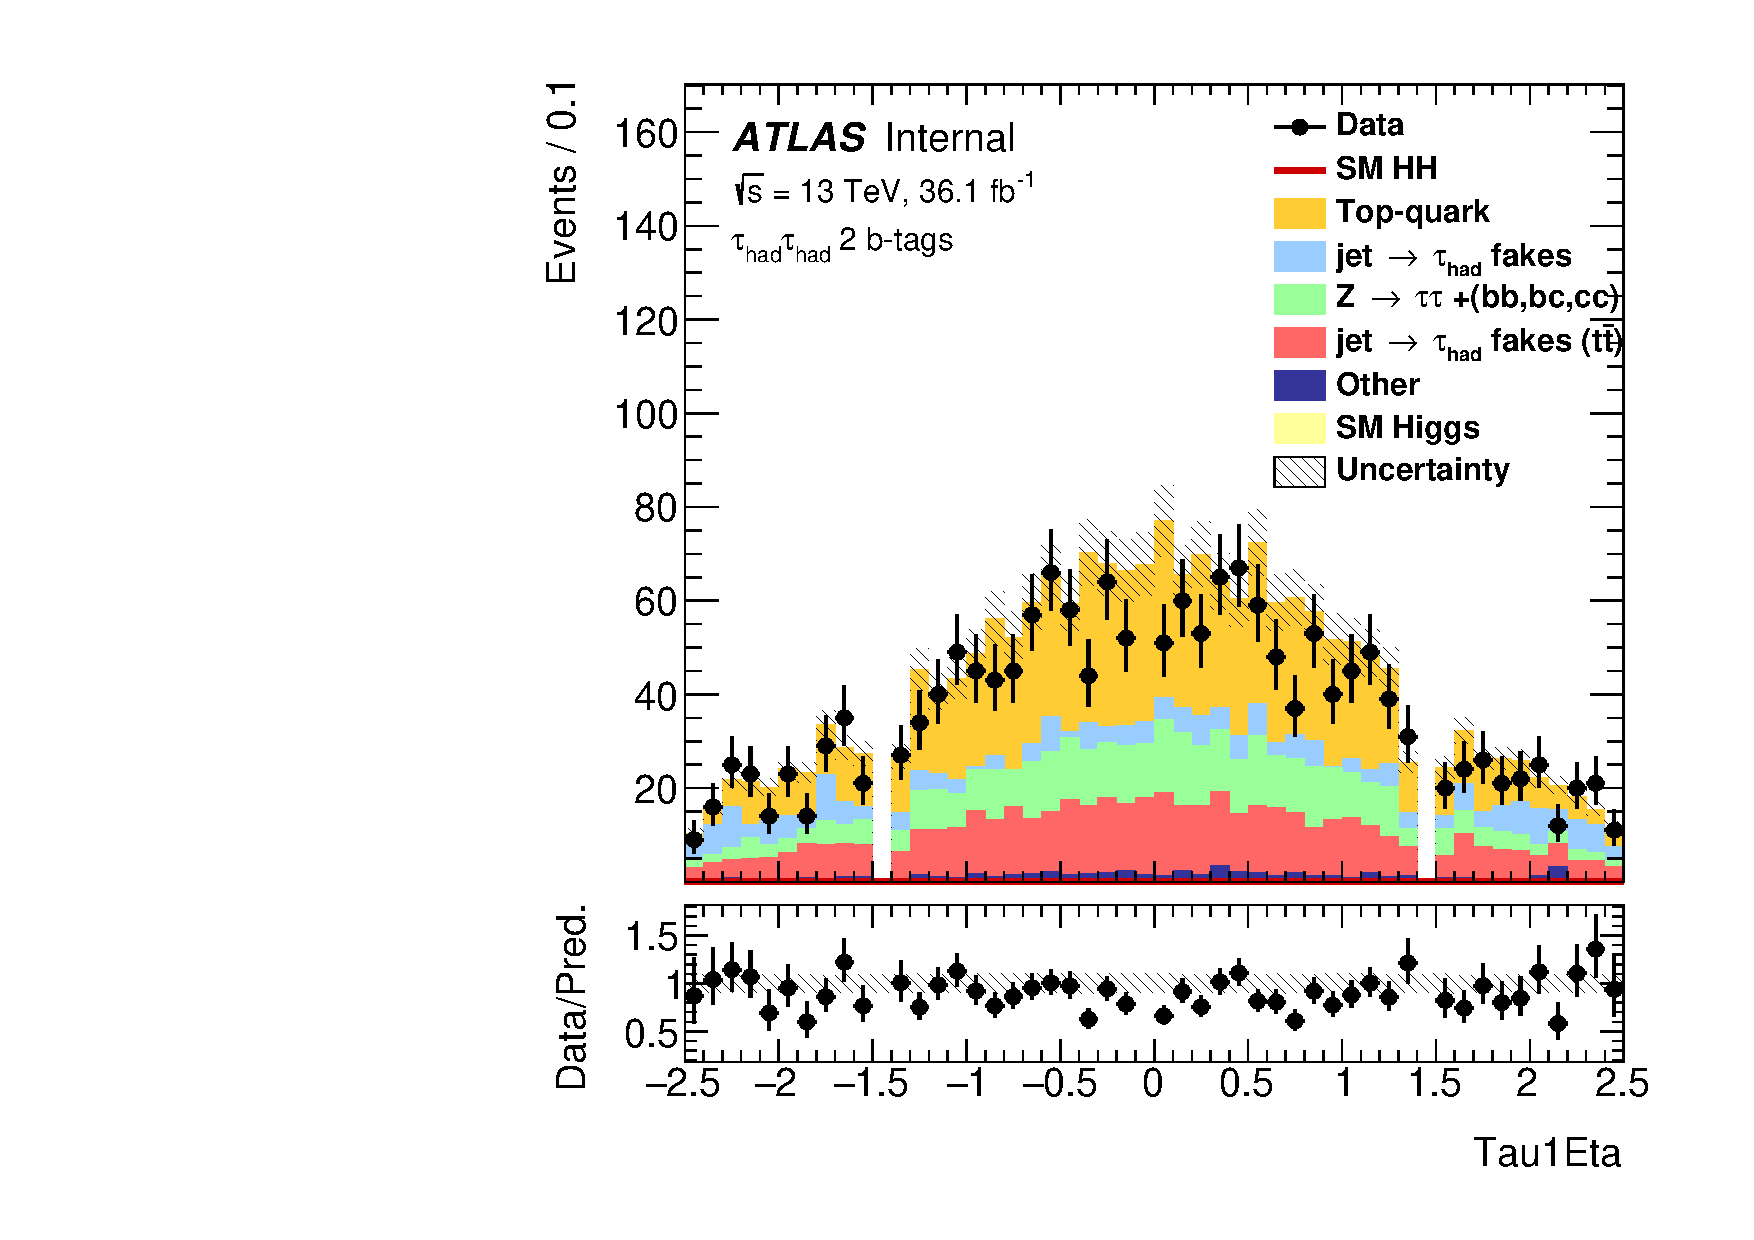
\includegraphics[width=.45\textwidth]{figures/selection/HadHad_HH/Plots2015/Region_BMin0_incJet1_distTau1Eta_J2_Y2015_DLLOS_T2_SpcTauHH_L0_Prefit.pdf}\\
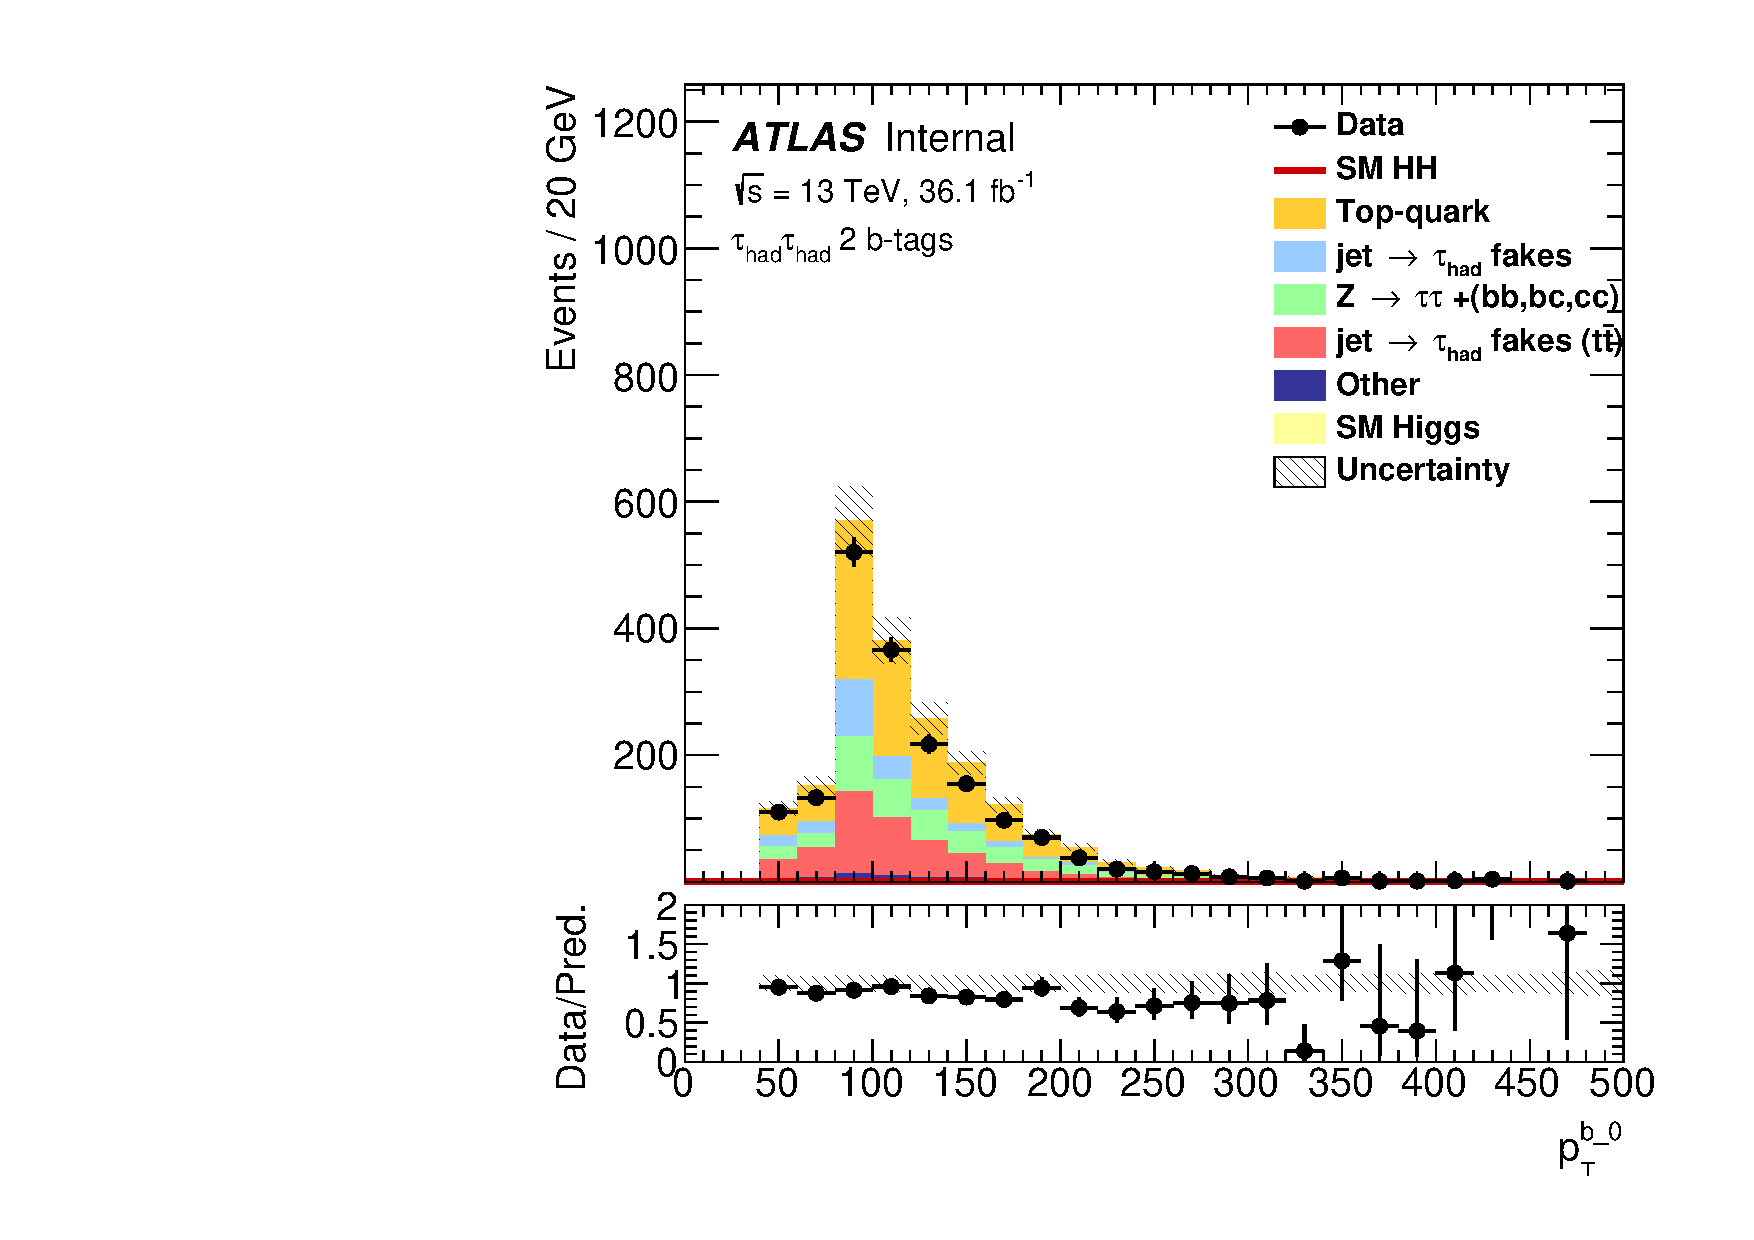
\includegraphics[width=.45\textwidth]{figures/selection/HadHad_HH/Plots2015/Region_BMin0_incJet1_distJet0Pt_J2_Y2015_DLLOS_T2_SpcTauHH_L0_Prefit.pdf}
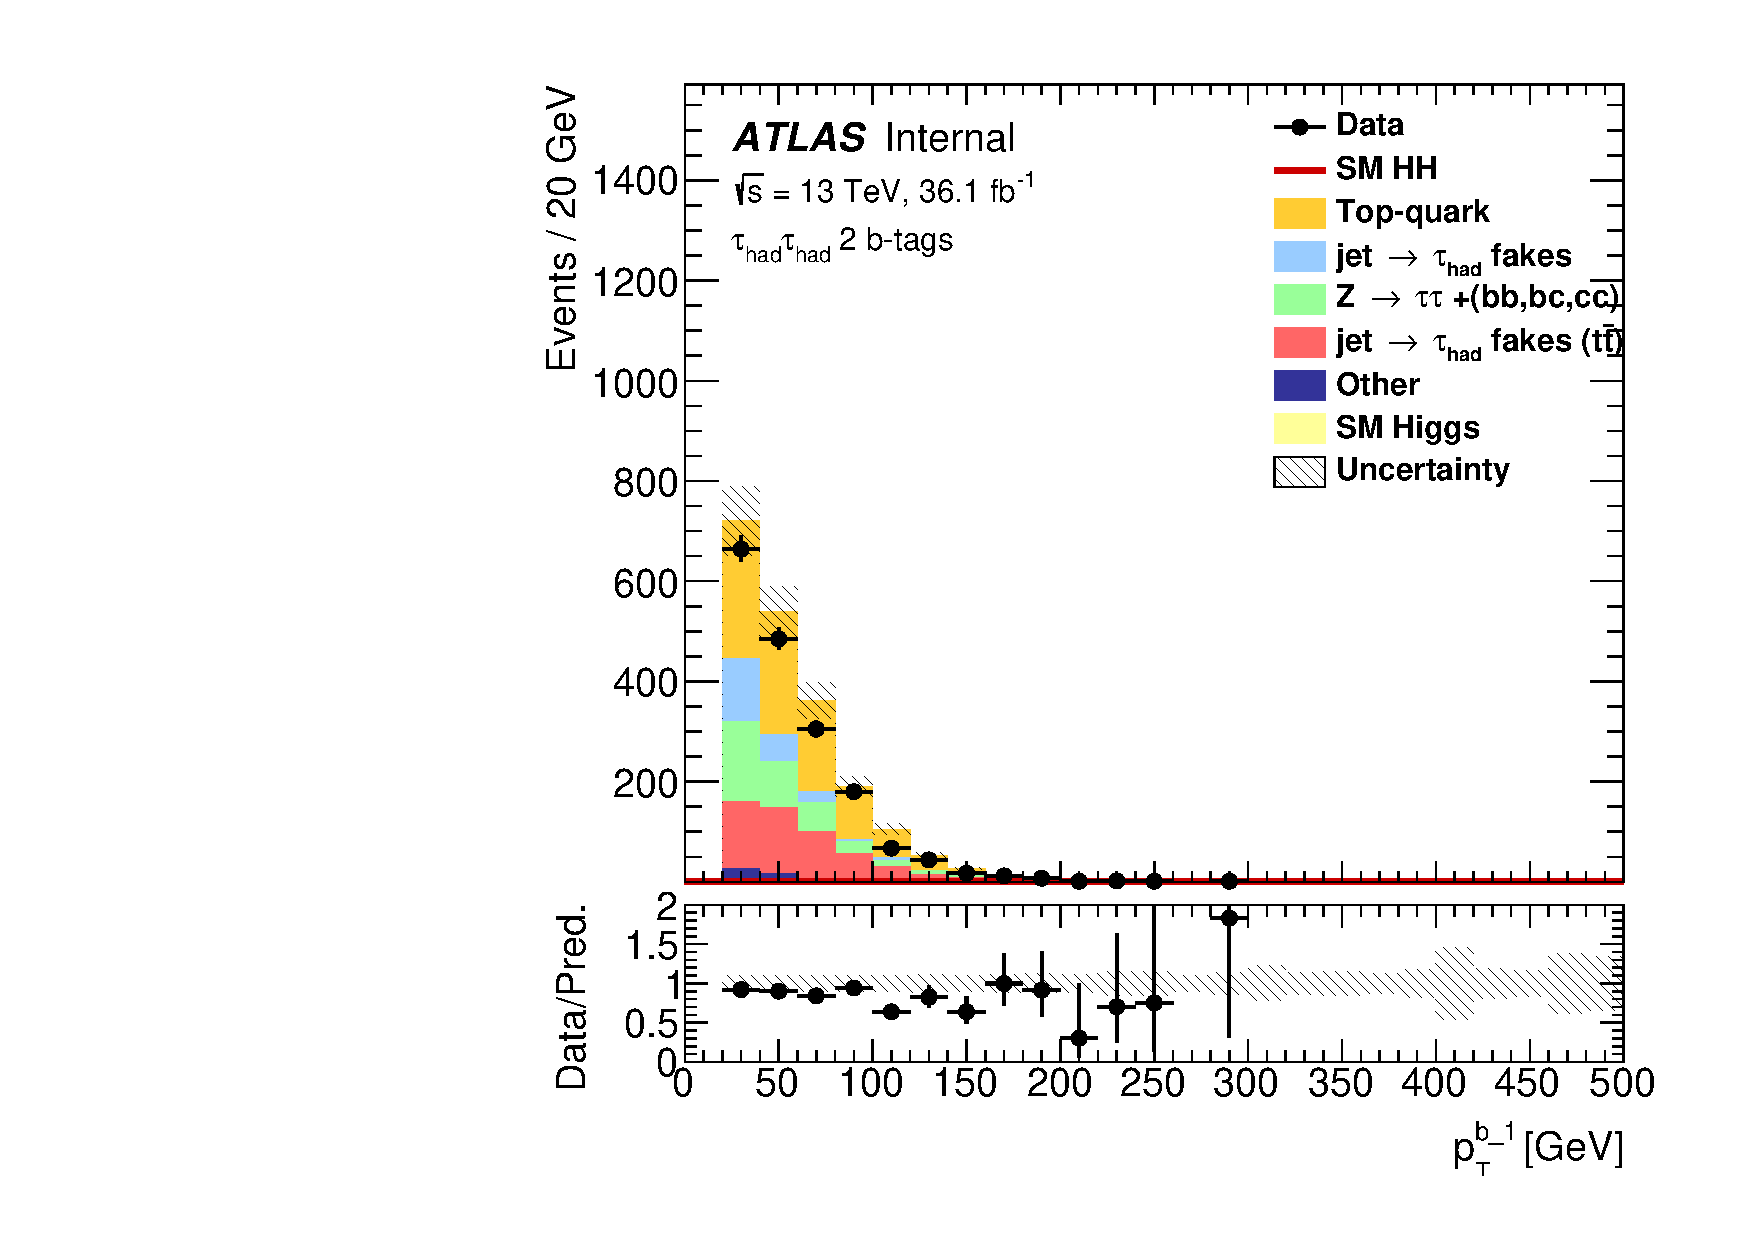
\includegraphics[width=.45\textwidth]{figures/selection/HadHad_HH/Plots2015/Region_BMin0_incJet1_distJet1Pt_J2_Y2015_DLLOS_T2_SpcTauHH_L0_Prefit.pdf}
\caption{Leading and sub-leading $\tau_{had}$ \pt and $\eta$ and $b$-jet \pt pre-fit
  distributions in the di-Higgs \hadhad signal region for the 2015-2016 data-taking period. (Inputs from 2021\_01\_15)}
\label{fig:HadHadPreselectionPtDistributions2015}
\end{figure}

\begin{figure}
\centering
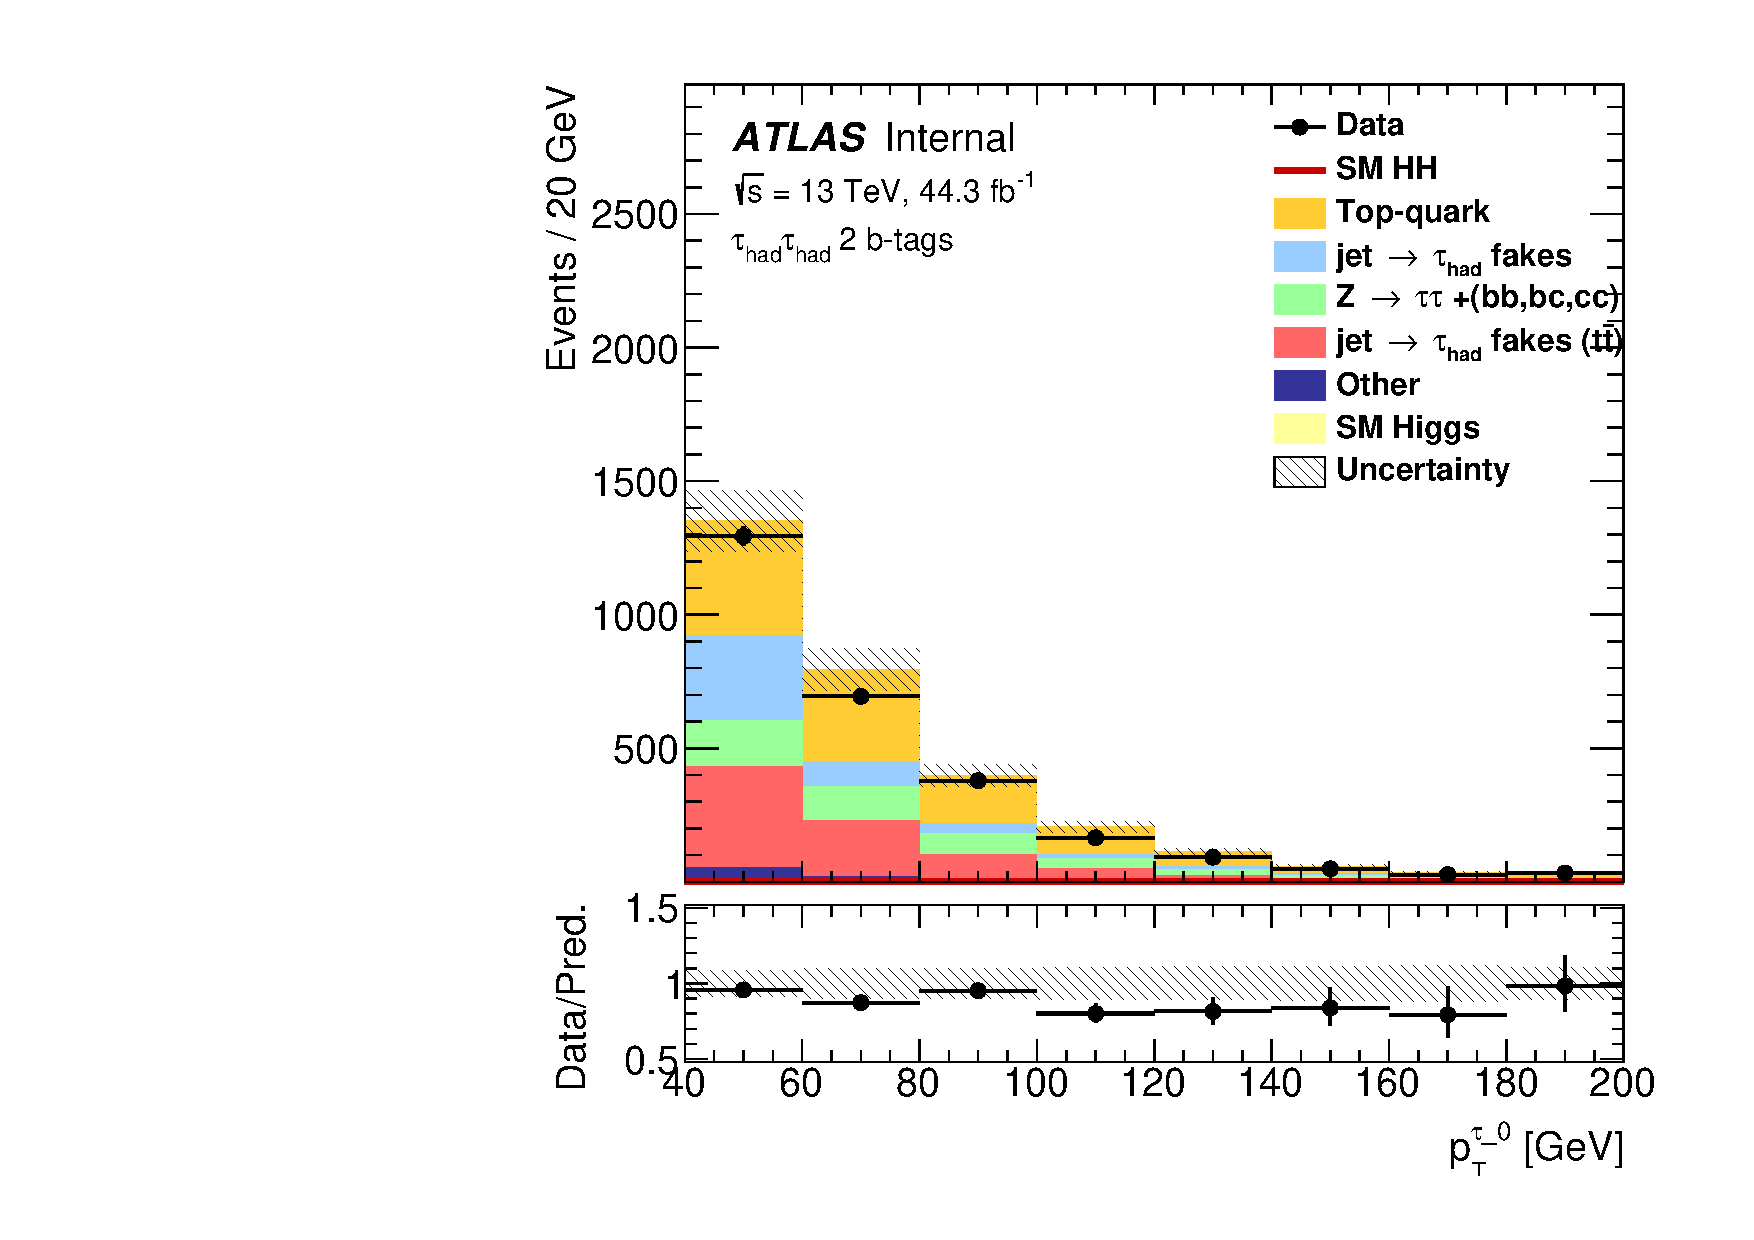
\includegraphics[width=.45\textwidth]{figures/selection/HadHad_HH/Plots2017/Region_BMin0_incJet1_distTau0Pt_J2_Y2015_DLLOS_T2_SpcTauHH_L0_Prefit.pdf}
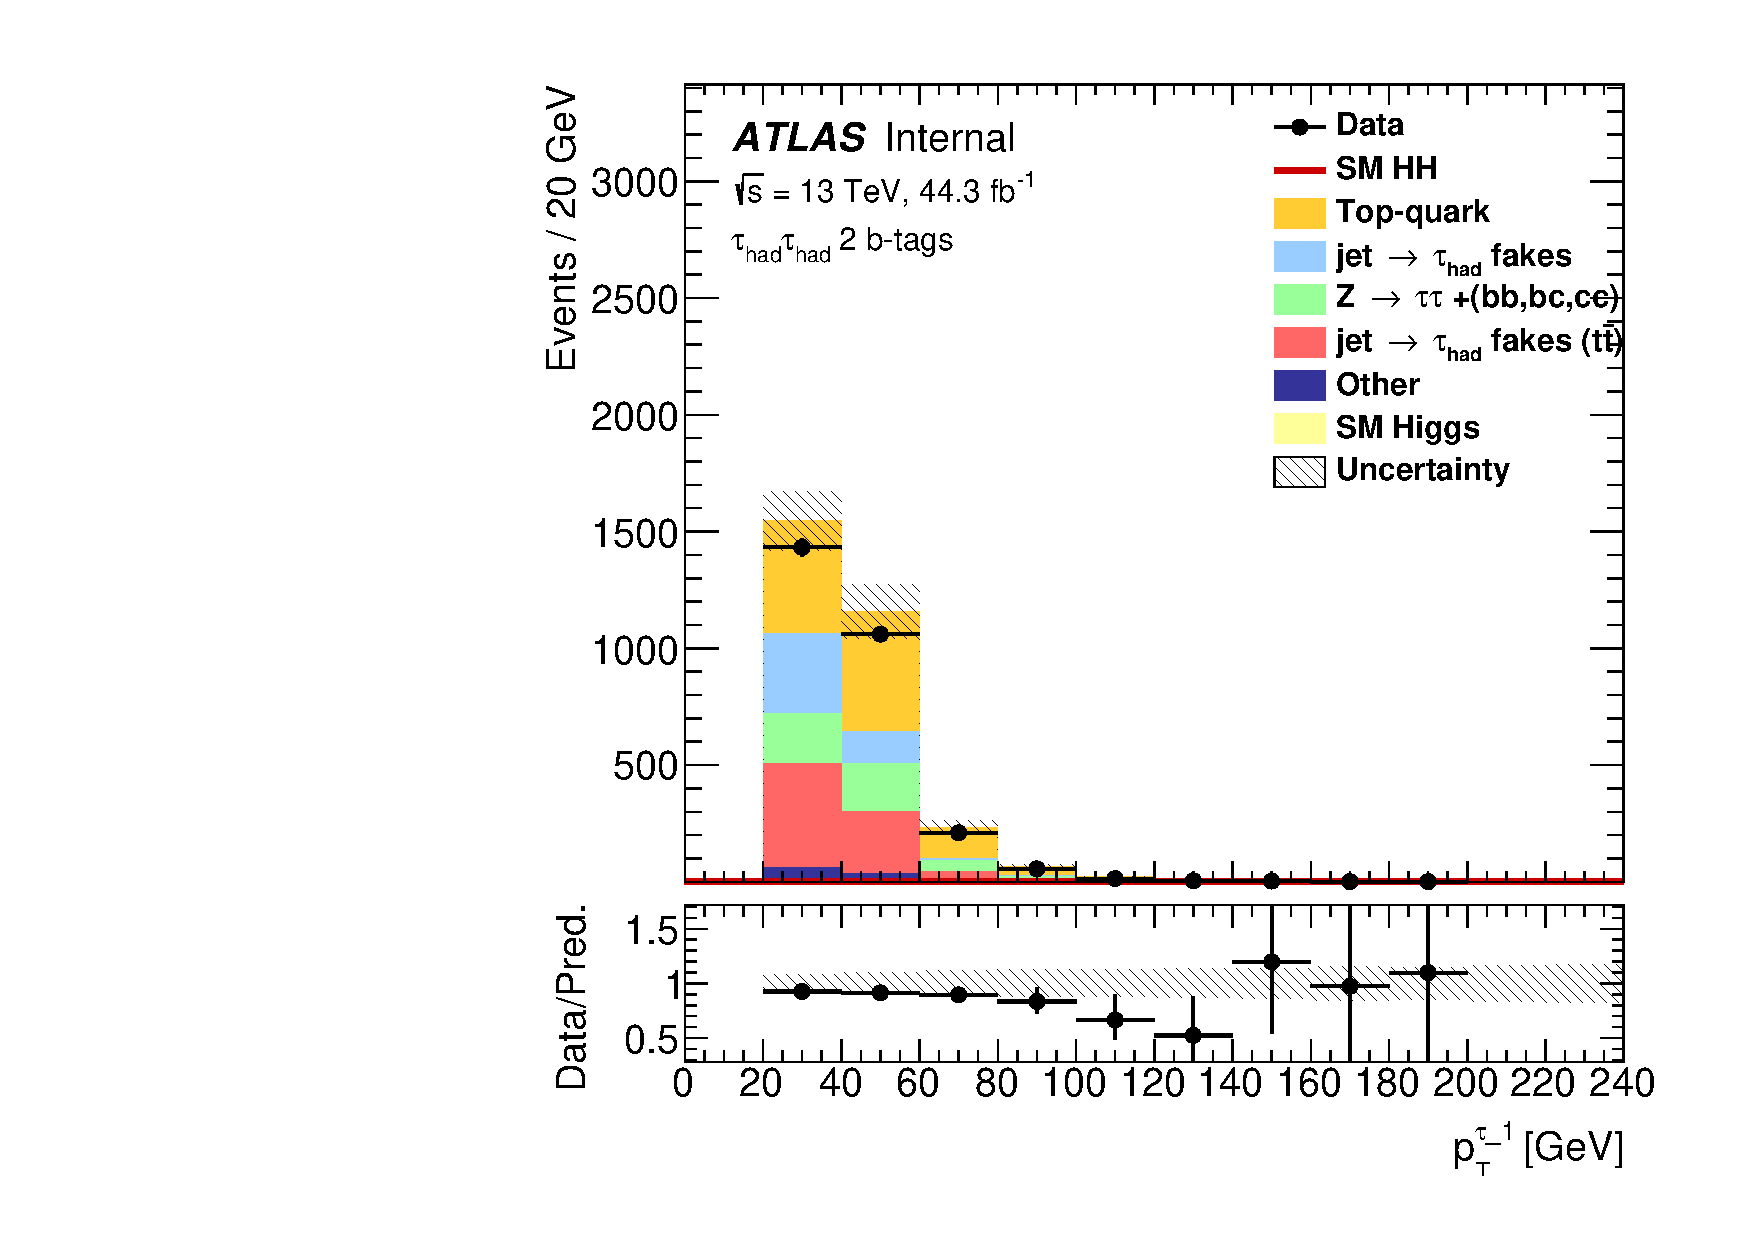
\includegraphics[width=.45\textwidth]{figures/selection/HadHad_HH/Plots2017/Region_BMin0_incJet1_distTau1Pt_J2_Y2015_DLLOS_T2_SpcTauHH_L0_Prefit.pdf}\\
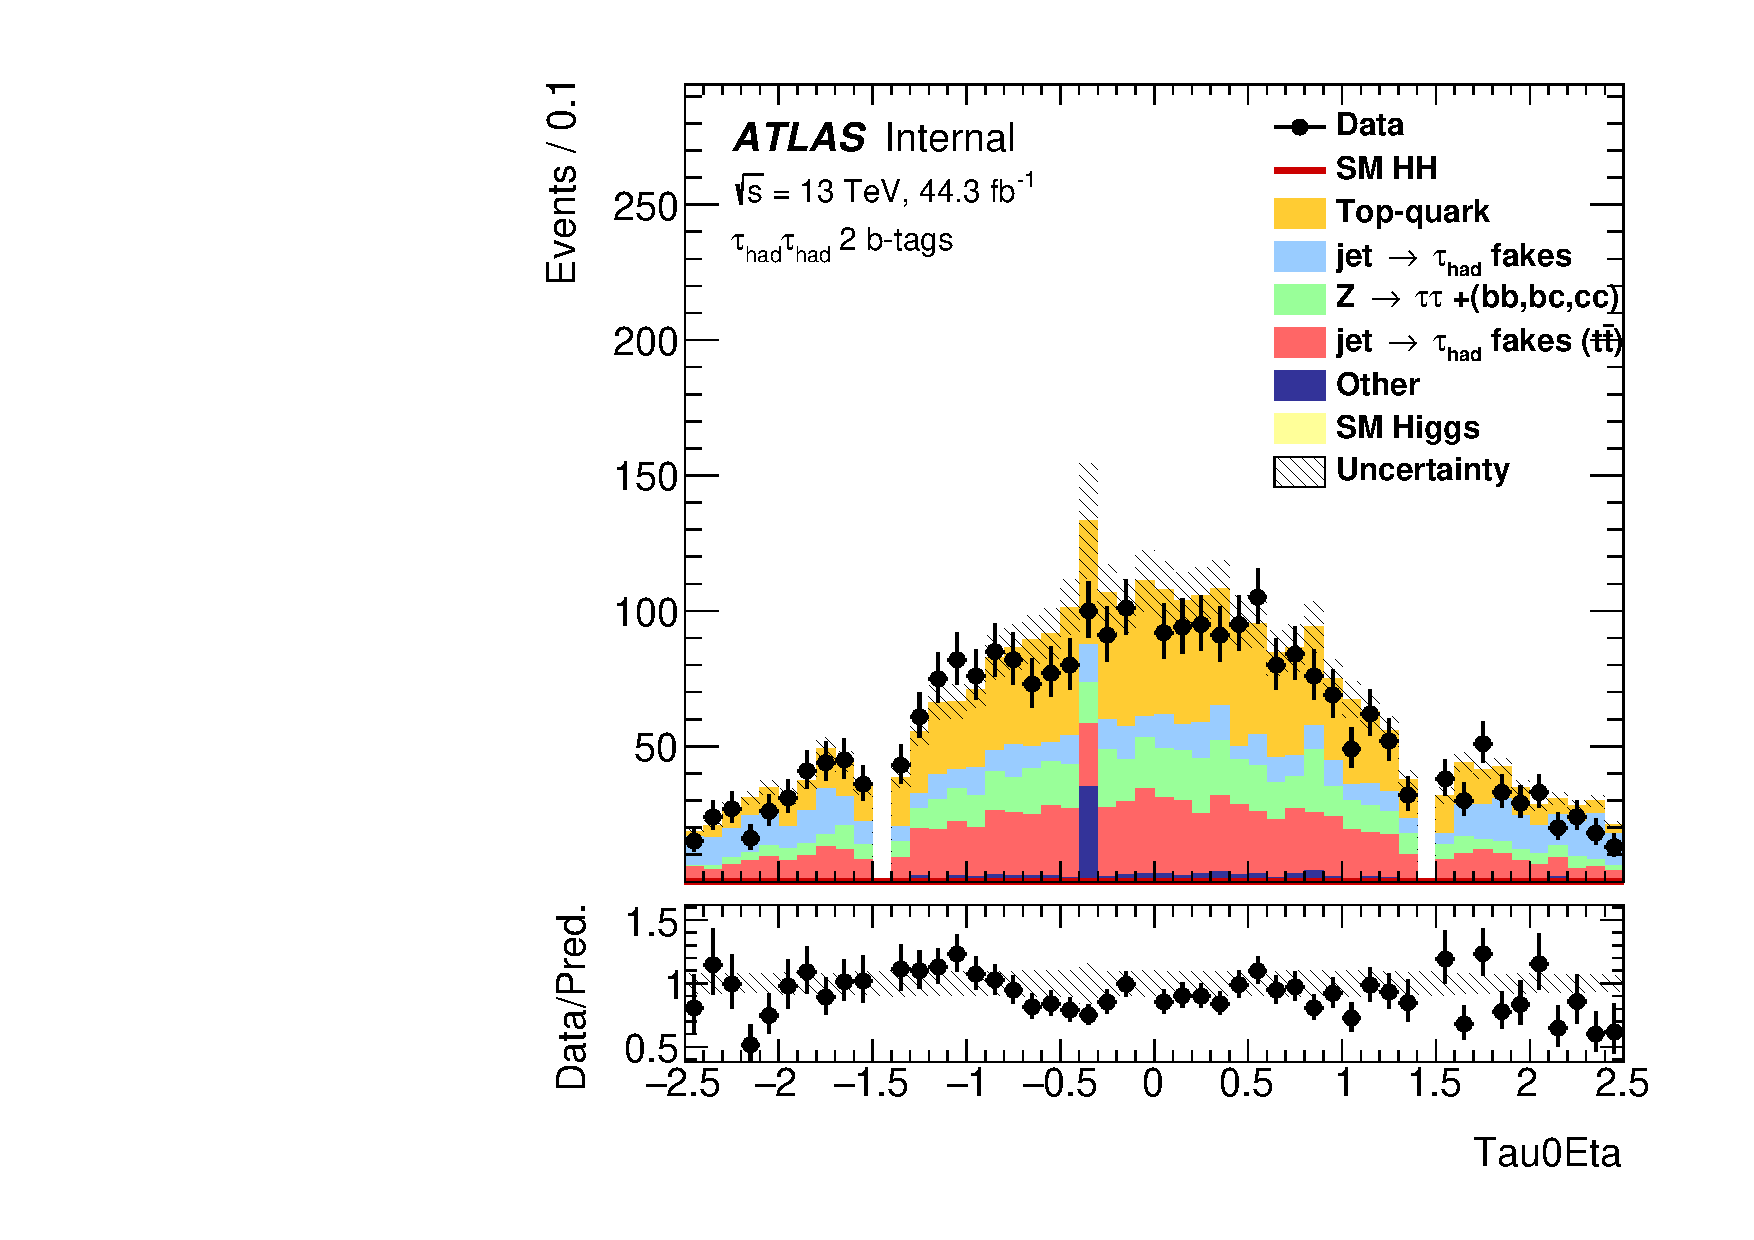
\includegraphics[width=.45\textwidth]{figures/selection/HadHad_HH/Plots2017/Region_BMin0_incJet1_distTau0Eta_J2_Y2015_DLLOS_T2_SpcTauHH_L0_Prefit.pdf}
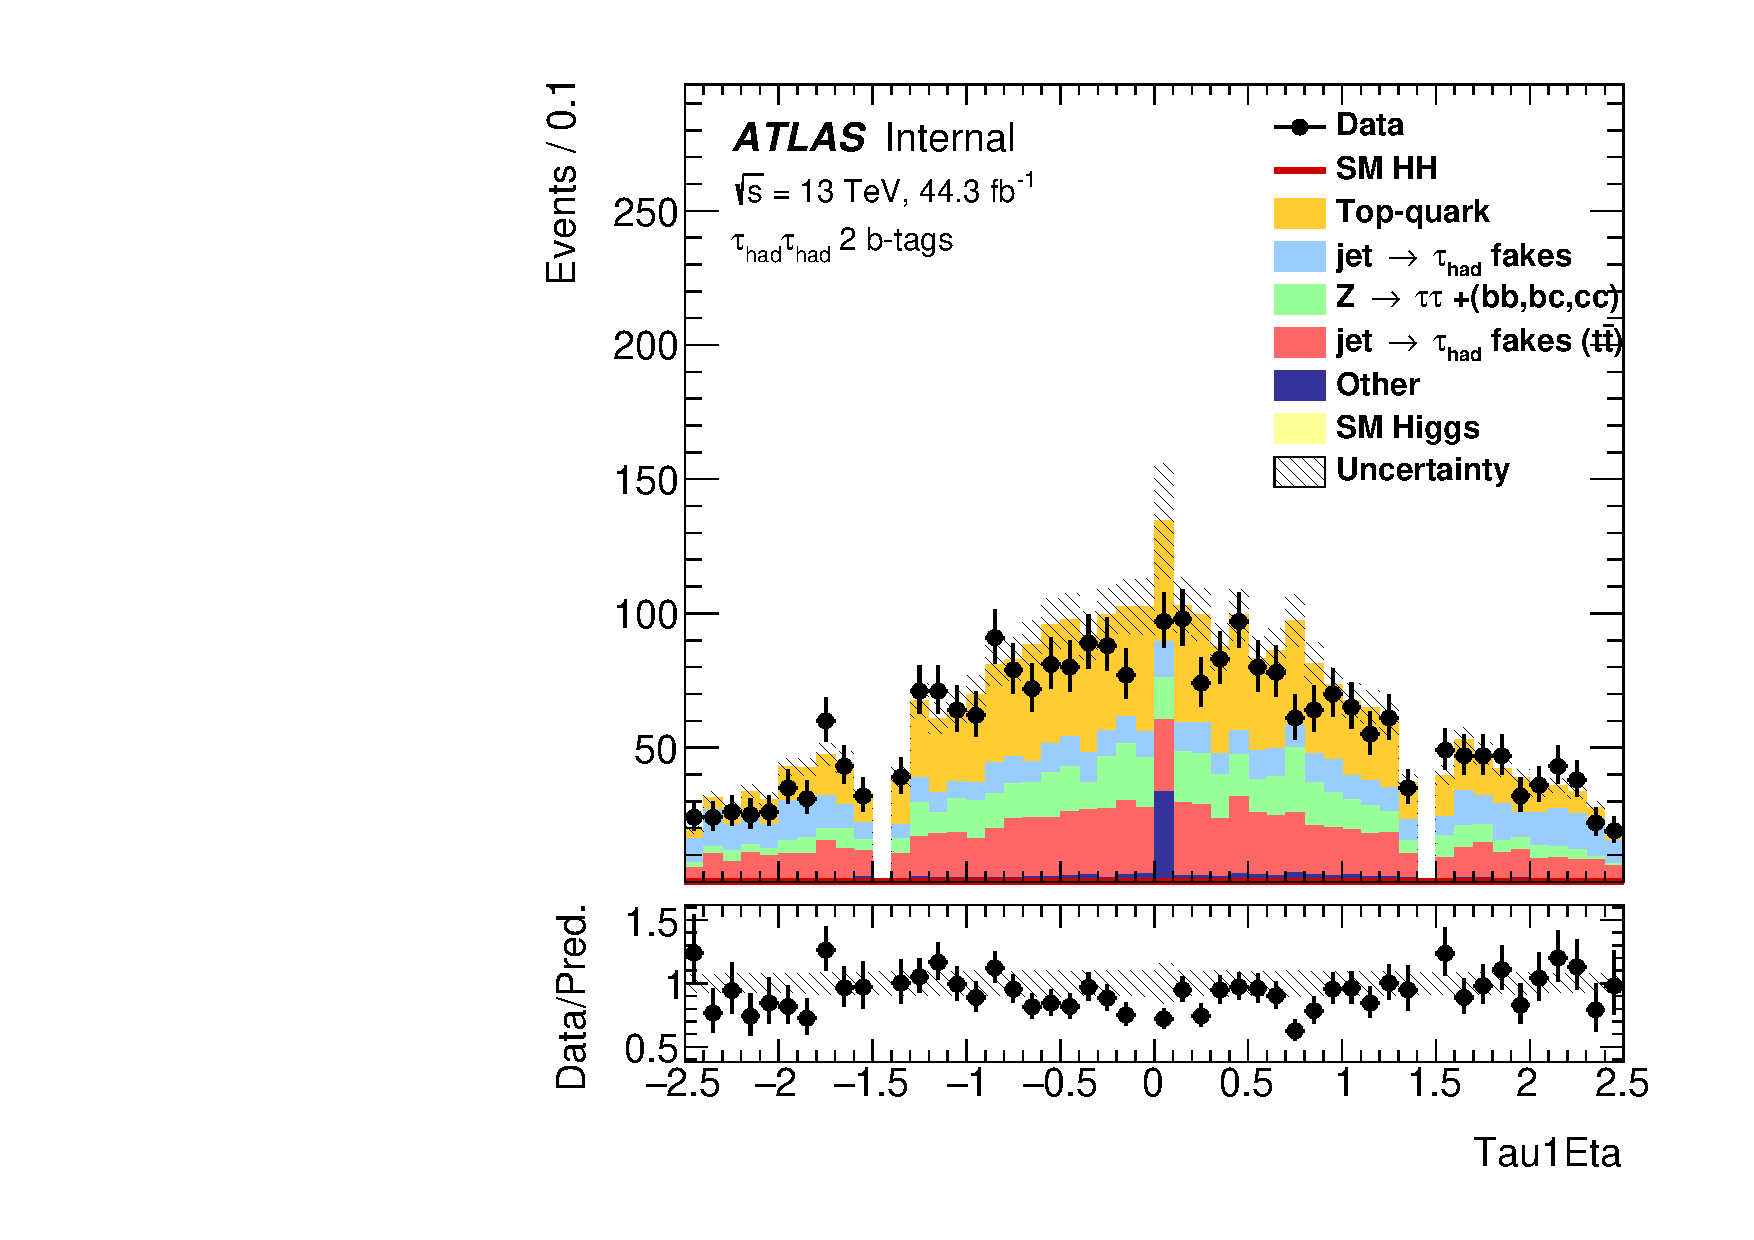
\includegraphics[width=.45\textwidth]{figures/selection/HadHad_HH/Plots2017/Region_BMin0_incJet1_distTau1Eta_J2_Y2015_DLLOS_T2_SpcTauHH_L0_Prefit.pdf}\\
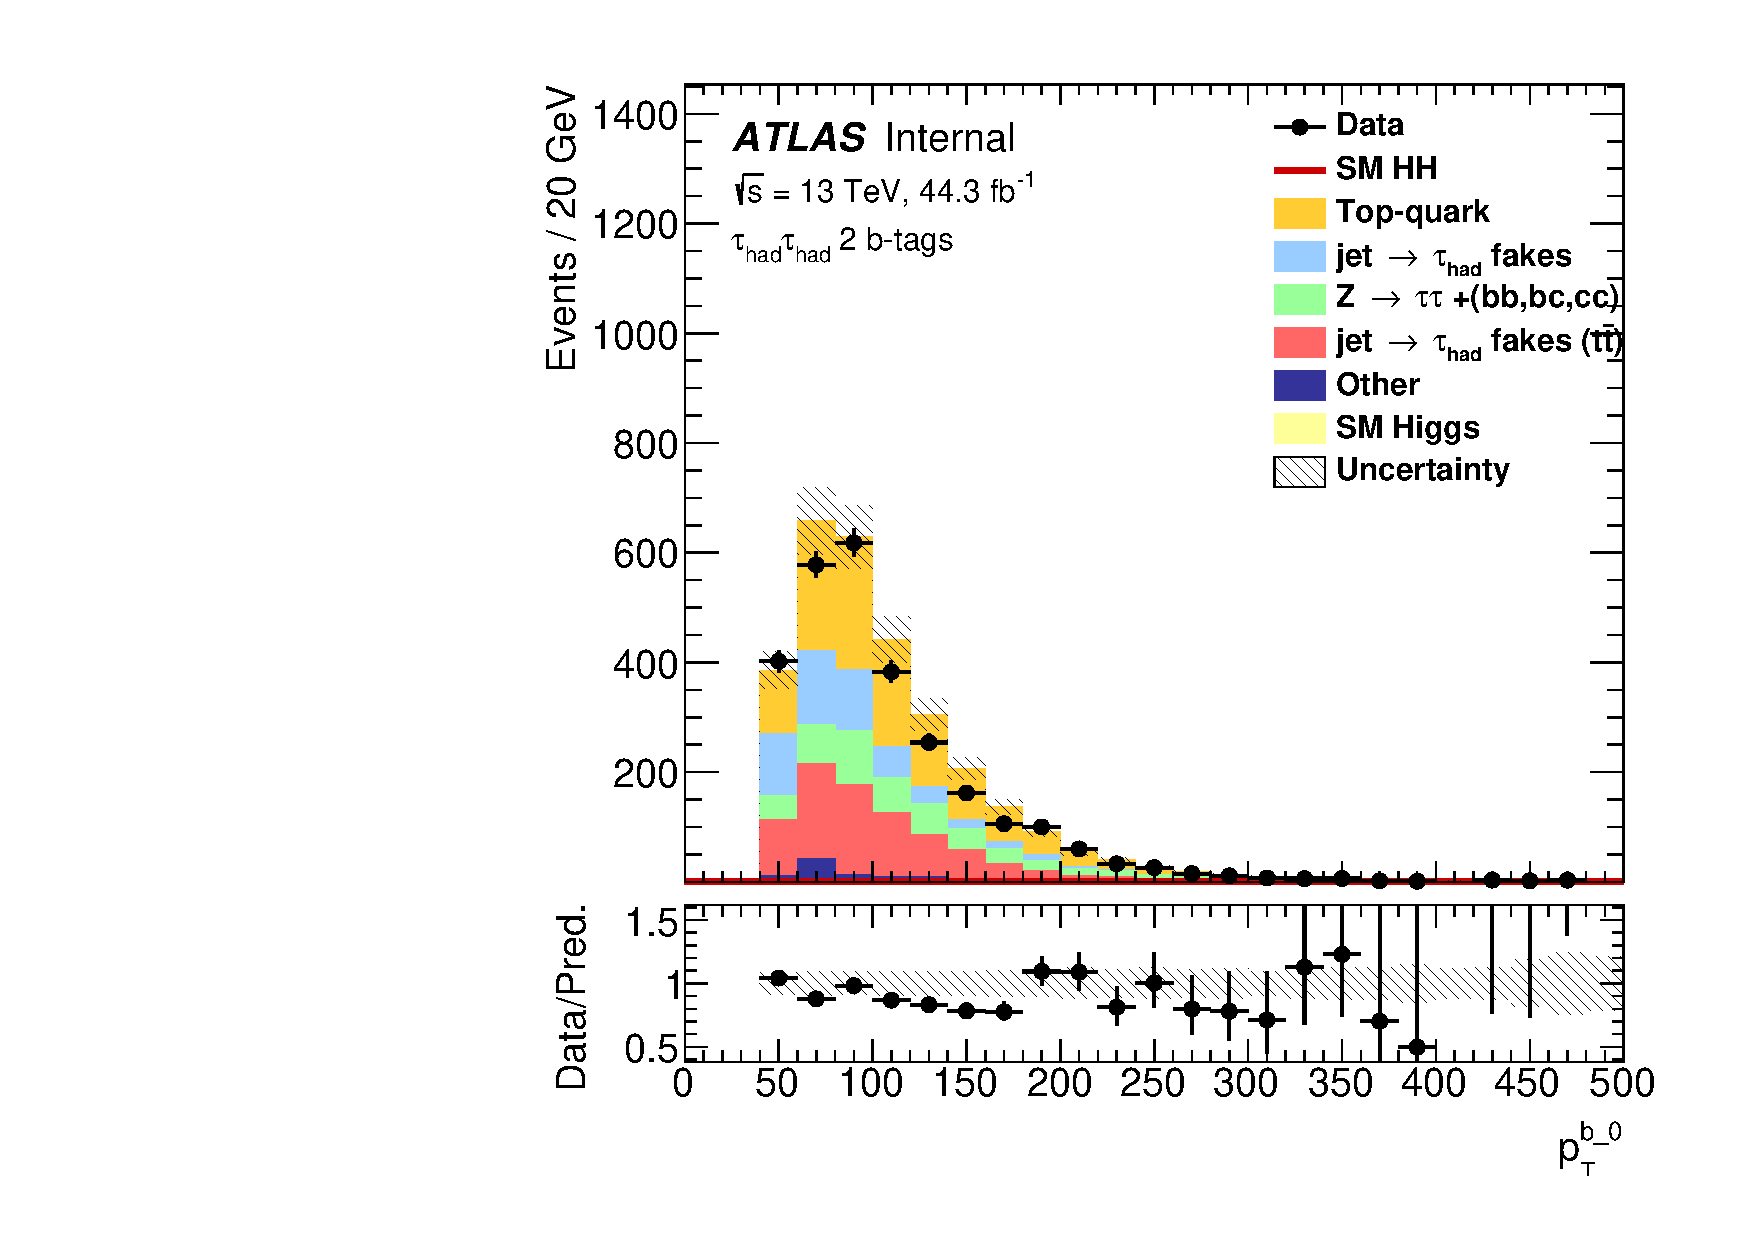
\includegraphics[width=.45\textwidth]{figures/selection/HadHad_HH/Plots2017/Region_BMin0_incJet1_distJet0Pt_J2_Y2015_DLLOS_T2_SpcTauHH_L0_Prefit.pdf}
\includegraphics[width=.45\textwidth]{figures/selection/HadHad_HH/Plots2017/Region_BMin0_incJet1_distJet1Pt_J2_Y2015_DLLOS_T2_SpcTauHH_L0_Prefit.pdf}
\caption{Leading and sub-leading $\tau_{had}$ \pt and $\eta$ and $b$-jet \pt pre-fit
  distributions in the di-Higgs \hadhad signal region for the 2017 data-taking period. (Inputs from 2021\_01\_15)}
\label{fig:HadHadPreselectionPtDistributions2017}
\end{figure}

\begin{figure}
\centering
\includegraphics[width=.45\textwidth]{figures/selection/HadHad_HH/Plots2018/Region_BMin0_incJet1_distTau0Pt_J2_Y2015_DLLOS_T2_SpcTauHH_L0_Prefit.pdf}
\includegraphics[width=.45\textwidth]{figures/selection/HadHad_HH/Plots2018/Region_BMin0_incJet1_distTau1Pt_J2_Y2015_DLLOS_T2_SpcTauHH_L0_Prefit.pdf}\\
\includegraphics[width=.45\textwidth]{figures/selection/HadHad_HH/Plots2018/Region_BMin0_incJet1_distTau0Eta_J2_Y2015_DLLOS_T2_SpcTauHH_L0_Prefit.pdf}
\includegraphics[width=.45\textwidth]{figures/selection/HadHad_HH/Plots2018/Region_BMin0_incJet1_distTau1Eta_J2_Y2015_DLLOS_T2_SpcTauHH_L0_Prefit.pdf}\\
\includegraphics[width=.45\textwidth]{figures/selection/HadHad_HH/Plots2018/Region_BMin0_incJet1_distJet0Pt_J2_Y2015_DLLOS_T2_SpcTauHH_L0_Prefit.pdf}
\includegraphics[width=.45\textwidth]{figures/selection/HadHad_HH/Plots2018/Region_BMin0_incJet1_distJet1Pt_J2_Y2015_DLLOS_T2_SpcTauHH_L0_Prefit.pdf}
\caption{Leading and sub-leading $\tau_{had}$ \pt and $\eta$ and $b$-jet \pt pre-fit
  distributions in the di-Higgs \hadhad signal region for the 2018 data-taking period. (Inputs from 2021\_01\_15)}
\label{fig:HadHadPreselectionPtDistributions2018}
\end{figure}

Table~\ref{tab:HadHadYields} reports the event yields after applying the $bb\hadhad$ event selection.

Figure~\ref{fig:HadHadPreselectionSignalAcceptance} shows the acceptance times efficiency of the \hadhad channel selection for the di-Higgs resonant signals as a function of the resonance mass. The acceptance times efficiency of the \hadhad channel selection for the non-resonant SM ggF di-Higgs signal is 4.08 \%. For the VBF production of the non-resonant di-Higgs signal, the acceptance times efficiency is 2.26 \%.

Comparison of the acceptance times efficiency in this channel of this new analysis to the old analysis explaining the improvements is given in Appendix~\ref{subsec:appendix_selection_sigacc_hadhad}.

\begin{figure}
\centering
\includegraphics[width=.65\textwidth]{figures/selection/HadHad_HH/acc_times_eff}
\caption{Acceptance times efficiency of the \hadhad channel selection for the di-Higgs resonant signals as a function of the resonance mass.}
\label{fig:HadHadPreselectionSignalAcceptance}
\end{figure}


\begin{table}[]
  \centering
  \scriptsize
\begin{tabular}{|c|c|c|c|c|}
\hline
Samplename      & Entries       & Integral      & Error         & Error/Integ. \\
\hline
Hhhbbtautau1600 & 6783          & 151.606       & 1.89591       & 0.0125055 \\
Hhhbbtautau1400 & 10335         & 228.557       & 2.31767       & 0.0101405 \\
Hhhbbtautau1200 & 16458         & 356.701       & 2.86756       & 0.00803913 \\
Hhhbbtautau1100 & 34553         & 396.142       & 2.21483       & 0.00559099 \\
Hhhbbtautau1000 & 39095         & 437.269       & 2.29697       & 0.00525299 \\
Hhhbbtautau900  & 38406         & 425.43        & 2.25069       & 0.00529038 \\
Hhhbbtautau800  & 46730         & 393.532       & 1.97188       & 0.00501073 \\
Hhhbbtautau700  & 42324         & 349.682       & 1.83682       & 0.00525283 \\
Hhhbbtautau600  & 35859         & 289.018       & 1.64761       & 0.00570073 \\
Hhhbbtautau550  & 32183         & 254.681       & 1.53096       & 0.00601127 \\
Hhhbbtautau500  & 28147         & 216.619       & 1.39304       & 0.00643082 \\
Hhhbbtautau450  & 29693         & 174.027       & 1.03694       & 0.0059585 \\
Hhhbbtautau400  & 22998         & 128.518       & 0.870567      & 0.0067739 \\
Hhhbbtautau375  & 19397         & 106.977       & 0.790256      & 0.00738715 \\
Hhhbbtautau350  & 25720         & 84.6505       & 0.54268       & 0.00641083 \\
Hhhbbtautau325  & 20369         & 64.58         & 0.465808      & 0.00721288 \\
Hhhbbtautau300  & 15098         & 45.8639       & 0.383928      & 0.00837103 \\
Hhhbbtautau280  & 14485         & 33.5209       & 0.286617      & 0.00855039 \\
Hhhbbtautau260  & 11709         & 25.815        & 0.246017      & 0.00952999 \\
Hhhbbtautau251  & 12621         & 27.2638       & 0.250045      & 0.00917132 \\
hhttbbVBFSM     & 37974         & 0.166899      & 0.000882937   & 0.00529025 \\
hhttbbggFSM     & 111552        & 5.40058       & 0.0193445     & 0.00358194 \\
\hline
Fake            & 119664        & 1354.66       & 25.8309       & 0.0190681 \\
ttbarSFFF       & 1510          & 358.921       & 10.1382       & 0.0282464 \\
ttbarSFFT       & 5468          & 698.522       & 10.2809       & 0.0147181 \\
ttbarSFTF       & 9223          & 1433.95       & 16.0457       & 0.0111899 \\
ttbar           & 22937         & 3580.69       & 24.734        & 0.00690762 \\
stopWt          & 1828          & 239.007       & 5.85533       & 0.0244986 \\
stopt           & 138           & 31.4158       & 3.04587       & 0.0969535 \\
stops           & 58            & 1.66692       & 0.231854      & 0.139092 \\
Zbb             & 30            & 1.23201       & 0.253941      & 0.20612 \\
Zbc             & 4             & 0.211169      & 0.129463      & 0.613078 \\
Zbl             & 0             & 0     & 0     & 0 \\
Zcc             & 0             & 0     & 0     & 0 \\
Zcl             & 0             & 0     & 0     & 0 \\
Zl              & 1             & 0.391639      & 0.391639      & 1 \\
Zttbb           & 27512         & 1332.46       & 16.4981       & 0.0123817 \\
Zttbc           & 2375          & 140.201       & 5.80802       & 0.0414263 \\
Zttbl           & 1544          & 54.8843       & 3.0808        & 0.0561327 \\
Zttcc           & 719           & 89.8517       & 12.1893       & 0.13566 \\
Zttcl           & 431           & 30.4873       & 3.82835       & 0.125572 \\
Zttl            & 195           & 23.8278       & 36.69         & 1.5398 \\
Wtt             & 457           & 52.269        & 6.50357       & 0.124425 \\
W               & 12            & 0.864665      & 0.292456      & 0.338231 \\
VBFHtautau      & 763           & 1.64109       & 0.0622571     & 0.0379364 \\
ggFHtautau      & 1155          & 14.054        & 0.542865      & 0.0386271 \\
ZHtautau        & 1729          & 8.01903       & 0.204466      & 0.0254976 \\
WHtautau        & 48            & 0.410149      & 0.0630599     & 0.153749 \\
ZHbb            & 62251         & 14.6234       & 0.216057      & 0.0147748 \\
WHbb            & 218           & 0.164501      & 0.0175373     & 0.106609 \\
WW              & 10            & 1.91138       & 0.728729      & 0.381258 \\
WZ              & 373           & 8.8442        & 0.743756      & 0.0840954 \\
ZZ              & 2382          & 33.2378       & 1.23828       & 0.0372553 \\
ttW             & 4850          & 13.6032       & 0.299571      & 0.0220222 \\
ttZ             & 34755         & 32.3468       & 0.482682      & 0.0149221 \\
ttH             & 25696         & 34.6773       & 0.249151      & 0.00718483 \\
\hline
bkg:            & 328336        & 9589.05  &&\\
data            & 8380          & 8380 && \\
\hline
\end{tabular}
\caption{Pre-fit event yields in the di-Higgs $bb\hadhad$ signal
  region. Here, Zttjj represents the processes as $Z\rightarrow\tau\tau + jj$,
whereas Zjj represents  $Z\rightarrow ee/\mu\mu + jj$. The yields for Zttbb, Zttbc and Zttcc are scaled by 1.3. (Inputs from 2021\_06\_17)}
\label{tab:HadHadYields}
\end{table}

The cutflows for non-resonant \hadhad SM ggF and VBF signal, as well as for resonant signals at various mass points are shown in Table~\ref{tab:SMHH_hadhad_cutflow} to Table~\ref{tab:X1000_hadhad_cutflow}.
% ggF SM HH
\begin{landscape}
\begin{table}
\centering

\begin{tabular}{|c|cc|cc|cc|}
\hline
Description & \multicolumn{2}{c|}{Number of events} & \multicolumn{2}{c|}{Efficiency [\%]} & \multicolumn{2}{c|}{Relative Efficiency [\%] }\\
\hline
& STT & DTT & STT &  DTT &  STT &  DTT \\
\hline
$HH$ & \multicolumn{2}{c|}{4314.87} & \multicolumn{2}{c|}{x} & \multicolumn{2}{c|}{x} \\
$HH\rightarrow bb\tau\tau$ & \multicolumn{2}{c|}{315.23} & \multicolumn{2}{c|}{x} & \multicolumn{2}{c|}{x} \\
$HH\rightarrow bb\tau_{h}\tau_{h}$ & \multicolumn{2}{c|}{132.32} & \multicolumn{2}{c|}{100.00} & \multicolumn{2}{c|}{100.00} \\
Generator filter & \multicolumn{2}{c|}{102.78} & \multicolumn{2}{c|}{77.68} & \multicolumn{2}{c|}{77.68} \\
Derivation skimming & \multicolumn{2}{c|}{88.28} & \multicolumn{2}{c|}{66.72} & \multicolumn{2}{c|}{85.89} \\
Object preselection & \multicolumn{2}{c|}{40.44} & \multicolumn{2}{c|}{30.56} & \multicolumn{2}{c|}{45.81} \\
\hline
Trigger selection (online+offline) & \multicolumn{2}{c|}{17.30} & \multicolumn{2}{c|}{13.08} & \multicolumn{2}{c|}{42.79} \\
Trigger category & 1.95 & 15.35 & 1.48 & 11.60 & 11.29 & 88.71 \\
\hline
Random $\tau$ selection & 1.93 & 15.31 & 1.46 & 11.57 & 99.03 & 99.78 \\
Object selection ($n_\tau=2$, further requirements on jets and tau-jet OLR) & 1.86 & 14.12 & 1.40 & 10.67 & 95.92 & 92.19 \\
Pileup Correction & 1.91 & 14.40 & 1.44 & 10.88 & x & x \\
2 Loose $\tau$s (one Loose $\tau$ already required in derivation) & 1.37 & 11.64 & 1.04 & 8.80 & 71.95 & 80.84 \\
Subleading $\tau$ \pt>25 GeV& 1.21 & 11.64 & 0.91 & 8.80 & 87.74 & x \\
\hline
MMC > 60 GeV& 1.15 & 11.40 & 0.87 & 8.62 & 95.40 & 97.98 \\
At least one jet with $\pT > 45$ GeV & 1.15 & 11.17 & 0.87 & 8.44 & 99.63 & 97.95 \\
DTT offline jet cuts & 1.15 & 9.95 & 0.87 & 7.52 & x & 89.05 \\
Scale Factors & 1.16 & 10.48 & 0.87 & 7.92 & x &x \\
Opposite charge sign & 1.14 & 10.34 & 0.86 & 7.82 & 98.14 & 98.71 \\
Both jets are b-tagged & 0.57 & 4.83 & 0.43 & 3.65 & 49.86 & 46.74 \\
\hline
\end{tabular}
\caption{Non-resonant \hadhad SM ggF signal cutflow (Powheg+Pythia8).}
\label{tab:SMHH_hadhad_cutflow}
\end{table}
\end{landscape}


% VBF SM HH
\begin{landscape}
\begin{table}
\centering

\begin{tabular}{|c|cc|cc|cc|}
\hline
Description & \multicolumn{2}{c|}{Number of events} & \multicolumn{2}{c|}{Efficiency [\%]} & \multicolumn{2}{c|}{Relative Efficiency [\%] }\\
\hline
& STT & DTT & STT &  DTT &  STT &  DTT \\
\hline
$HH$ & \multicolumn{2}{c|}{239.85} & \multicolumn{2}{c|}{x} & \multicolumn{2}{c|}{x} \\
$HH\rightarrow bb\tau\tau$ & \multicolumn{2}{c|}{17.52} & \multicolumn{2}{c|}{x} & \multicolumn{2}{c|}{x} \\
$HH\rightarrow bb\tau_{h}\tau_{h}$ & \multicolumn{2}{c|}{7.36} & \multicolumn{2}{c|}{100.00} & \multicolumn{2}{c|}{100.00} \\
Generator filter & \multicolumn{2}{c|}{5.00} & \multicolumn{2}{c|}{67.99} & \multicolumn{2}{c|}{67.99} \\
Derivation skimming & \multicolumn{2}{c|}{4.24} & \multicolumn{2}{c|}{57.61} & \multicolumn{2}{c|}{84.73} \\
Object preselection & \multicolumn{2}{c|}{1.89} & \multicolumn{2}{c|}{25.69} & \multicolumn{2}{c|}{44.59} \\
\hline
Trigger selection (online+offline) & \multicolumn{2}{c|}{0.74} & \multicolumn{2}{c|}{10.11} & \multicolumn{2}{c|}{39.36} \\
Trigger category & 0.06 & 0.69 & 0.79 & 9.32 & 7.82  & 92.18 \\
\hline
Random $\tau$ selection & 0.06 & 0.68 & 0.78 & 9.28 & 98.64 & 99.55 \\
Object selection ($n_\tau=2$, further requirements on jets and tau-jet OLR) & 0.05 & 0.59 & 0.72 & 7.99 & 92.33 & 86.07 \\
Pileup Correction & 0.05 & 0.60 & 0.74 & 8.13 & x	  & x\\
2 Loose $\tau$s (one Loose $\tau$ already required in derivation) & 0.04 & 0.48 & 0.56 & 6.54 & 74.81 & 80.37 \\
Subleading $\tau$ \pt>25 GeV& 0.04 & 0.48 & 0.49 & 6.54 & 88.41 & x\\
\hline
MMC > 60 GeV& 0.03 & 0.47 & 0.47 & 6.37 & 95.60 & 97.52 \\
At least one jet with $\pT > 45$ GeV & 0.03 & 0.45 & 0.46 & 6.07 & 98.65 & 95.26 \\
DTT offline jet cuts & 0.03 & 0.35 & 0.46 & 4.80 & x	  & 78.99 \\
Scale Factors & 0.03 & 0.37 & 0.47 & 5.03 & x	  & x\\
Opposite charge sign & 0.03 & 0.36 & 0.46 & 4.94 & 97.86 & 98.19 \\
Both jets are b-tagged & 0.01 & 0.15 & 0.20 & 2.07 & 42.67 & 41.98 \\
\hline
\end{tabular}
\caption{Non-resonant \hadhad SM VBF signal cutflow.}
\label{tab:SMVBFHH_hadhad_cutflow}
\end{table}
\end{landscape}


% X300
\begin{landscape}
\begin{table}
\centering

\begin{tabular}{|c|cc|cc|cc|}
\hline
Description & \multicolumn{2}{c|}{Number of events} & \multicolumn{2}{c|}{Efficiency [\%]} & \multicolumn{2}{c|}{Relative Efficiency [\%] }\\
\hline
& STT & DTT & STT &  DTT &  STT &  DTT \\
\hline
$HH$ & \multicolumn{2}{c|}{138965.16} & \multicolumn{2}{c|}{x} & \multicolumn{2}{c|}{x} \\
$HH\rightarrow bb\tau\tau$ & \multicolumn{2}{c|}{10152.27} & \multicolumn{2}{c|}{x} & \multicolumn{2}{c|}{x} \\
$HH\rightarrow bb\tau_{h}\tau_{h}$ & \multicolumn{2}{c|}{4261.66} & \multicolumn{2}{c|}{100.00} & \multicolumn{2}{c|}{100.00} \\
Generator filter & \multicolumn{2}{c|}{2652.79} & \multicolumn{2}{c|}{62.25} & \multicolumn{2}{c|}{62.25} \\
Derivation skimming & \multicolumn{2}{c|}{2168.46} & \multicolumn{2}{c|}{50.88} & \multicolumn{2}{c|}{81.74} \\
Object preselection & \multicolumn{2}{c|}{924.99} & \multicolumn{2}{c|}{21.70} & \multicolumn{2}{c|}{42.66} \\
\hline
Trigger selection (online+offline) & \multicolumn{2}{c|}{278.89} & \multicolumn{2}{c|}{6.54} & \multicolumn{2}{c|}{30.15} \\
Trigger category & 0.63 & 278.26 & 0.01 & 6.53 & 0.23   & 99.77  \\
\hline
Random $\tau$ selection & 0.63 & 277.68 & 0.01 & 6.52 & 99.55  & 99.79  \\
Object selection ($n_\tau=2$, further requirements on jets and tau-jet OLR) & 0.58 & 251.00 & 0.01 & 5.89 & 92.79  & 90.39  \\
Pileup Correction & 0.65 & 256.04 & 0.02 & 6.01 & x      & x \\
2 Loose $\tau$s (one Loose $\tau$ already required in derivation) & 0.43 & 200.67 & 0.01 & 4.71 & 66.48  & 78.38  \\
Subleading $\tau$ \pt>25 GeV& 0.32 & 200.67 & 0.01 & 4.71 & 74.60  & x \\
\hline
MMC > 60 GeV& 0.32 & 198.33 & 0.01 & 4.65 & 98.85  & 98.83  \\
At least one jet with $\pT > 45$ GeV & 0.29 & 179.85 & 0.01 & 4.22 & 90.34  & 90.68  \\
DTT offline jet cuts & 0.29 & 104.73 & 0.01 & 2.46 & x      & 58.23  \\
Scale Factors & 0.28 & 106.45 & 0.01 & 2.50 & x      & x \\
Opposite charge sign & 0.28 & 105.04 & 0.01 & 2.46 & 100.00 & 98.68  \\
Both jets are b-tagged & 0.13 & 45.73  & 0.00 & 1.07 & 47.49  & 43.54  \\
\hline
\end{tabular}
\caption{300~GeV resonant \hadhad signal cutflow. Assuming $\sigma(pp\rightarrow X\rightarrow HH)=1$~pb}
\label{tab:X300_hadhad_cutflow}
\end{table}
\end{landscape}


% X500
\begin{landscape}
\begin{table}
\centering

\begin{tabular}{|c|cc|cc|cc|}
\hline
Description & \multicolumn{2}{c|}{Number of events} & \multicolumn{2}{c|}{Efficiency [\%]} & \multicolumn{2}{c|}{Relative Efficiency [\%] }\\
\hline
& STT & DTT & STT &  DTT &  STT &  DTT \\
\hline
$HH$ & \multicolumn{2}{c|}{138965.16} & \multicolumn{2}{c|}{x} & \multicolumn{2}{c|}{x} \\
$HH\rightarrow bb\tau\tau$ & \multicolumn{2}{c|}{10152.27} & \multicolumn{2}{c|}{x} & \multicolumn{2}{c|}{x} \\
$HH\rightarrow bb\tau_{h}\tau_{h}$ & \multicolumn{2}{c|}{4261.66} & \multicolumn{2}{c|}{100.00} & \multicolumn{2}{c|}{100.00} \\
Generator filter & \multicolumn{2}{c|}{3256.65} & \multicolumn{2}{c|}{76.42} & \multicolumn{2}{c|}{76.42} \\
Derivation skimming & \multicolumn{2}{c|}{2843.20} & \multicolumn{2}{c|}{66.72} & \multicolumn{2}{c|}{87.30} \\
Object preselection & \multicolumn{2}{c|}{1364.93} & \multicolumn{2}{c|}{32.03} & \multicolumn{2}{c|}{48.01} \\
\hline
Trigger selection (online+offline) & \multicolumn{2}{c|}{645.23} & \multicolumn{2}{c|}{15.14} & \multicolumn{2}{c|}{47.27} \\
Trigger category & 56.96 & 588.27 & 1.34 & 13.80 & 8.83  & 91.17  \\
\hline
Random $\tau$ selection & 56.56 & 587.17 & 1.33 & 13.78 & 99.29 & 99.81  \\
Object selection ($n_\tau=2$, further requirements on jets and tau-jet OLR) & 54.37 & 551.63 & 1.28 & 12.94 & 96.13 & 93.95  \\
Pileup Correction & 53.43 & 576.13 & 1.25 & 13.52 & x     & x \\
2 Loose $\tau$s (one Loose $\tau$ already required in derivation) & 38.26 & 474.59 & 0.90 & 11.14 & 71.60 & 82.38  \\
Subleading $\tau$ \pt>25 GeV& 31.28 & 474.59 & 0.73 & 11.14 & 81.76 & x \\
\hline
MMC > 60 GeV& 30.09 & 465.55 & 0.71 & 10.92 & 96.20 & 98.09  \\
At least one jet with $\pT > 45$ GeV & 29.85 & 460.32 & 0.70 & 10.80 & 99.18 & 98.88  \\
DTT offline jet cuts & 29.85 & 434.24 & 0.70 & 10.19 & x     & 94.33  \\
Scale Factors & 29.65 & 452.56 & 0.70 & 10.62 & x     & x \\
Opposite charge sign & 28.98 & 446.93 & 0.68 & 10.49 & 97.71 & 98.76  \\
Both jets are b-tagged & 13.37 & 203.25 & 0.31 & 4.77  & 46.13 & 45.48  \\
\hline
\end{tabular}
\caption{500~GeV resonant \hadhad signal cutflow. Assuming $\sigma(pp\rightarrow X\rightarrow HH)=1$~pb}
\label{tab:X500_hadhad_cutflow}
\end{table}
\end{landscape}


% X1000
\begin{landscape}
\begin{table}
\centering

\begin{tabular}{|c|cc|cc|cc|}
\hline
Description & \multicolumn{2}{c|}{Number of events} & \multicolumn{2}{c|}{Efficiency [\%]} & \multicolumn{2}{c|}{Relative Efficiency [\%] }\\
\hline
& STT & DTT & STT &  DTT &  STT &  DTT \\
\hline
$HH$ & \multicolumn{2}{c|}{138965.16} & \multicolumn{2}{c|}{x} & \multicolumn{2}{c|}{x} \\
$HH\rightarrow bb\tau\tau$ & \multicolumn{2}{c|}{10152.27} & \multicolumn{2}{c|}{x} & \multicolumn{2}{c|}{x} \\
$HH\rightarrow bb\tau_{h}\tau_{h}$ & \multicolumn{2}{c|}{4261.66} & \multicolumn{2}{c|}{100.00} & \multicolumn{2}{c|}{100.00} \\
Generator filter & \multicolumn{2}{c|}{3750.86} & \multicolumn{2}{c|}{88.01} & \multicolumn{2}{c|}{88.01} \\
Derivation skimming & \multicolumn{2}{c|}{3330.25} & \multicolumn{2}{c|}{78.14} & \multicolumn{2}{c|}{88.79} \\
Object preselection & \multicolumn{2}{c|}{1753.58} & \multicolumn{2}{c|}{41.15} & \multicolumn{2}{c|}{52.661} \\
\hline
Trigger selection (online+offline) & \multicolumn{2}{c|}{1232.55} & \multicolumn{2}{c|}{28.92} & \multicolumn{2}{c|}{70.29} \\
Trigger category & 779.77 & 452.78 & 18.30 & 10.62 & 63.26 & 36.74 \\
\hline
Random $\tau$ selection & 774.73 & 451.99 & 18.18 & 10.61 & 99.35 & 99.83 \\
Object selection ($n_\tau=2$, further requirements on jets and tau-jet OLR) & 761.35 & 437.79 & 17.87 & 10.27 & 98.27 & 96.86 \\
Pileup Correction & 774.49 & 450.27 & 18.17 & 10.57 & x     & x\\
2 Loose $\tau$s (one Loose $\tau$ already required in derivation) & 587.02 & 384.98 & 13.77 & 9.03  & 75.80 & 85.50 \\
Subleading $\tau$ \pt>25 GeV& 555.91 & 384.98 & 13.04 & 9.03  & 94.70 & x\\
\hline
MMC > 60 GeV& 530.45 & 371.21 & 12.45 & 8.71  & 95.42 & 96.42 \\
At least one jet with $\pT > 45$ GeV & 530.07 & 369.78 & 12.44 & 8.68  & 99.93 & 99.62 \\
DTT offline jet cuts & 530.07 & 353.30 & 12.44 & 8.29  & x     & 95.54 \\
Scale Factors & 531.29 & 373.62 & 12.47 & 8.77  & x     & x\\
Opposite charge sign & 520.97 & 367.95 & 12.22 & 8.63  & 98.06 & 98.48 \\
Both jets are b-tagged & 263.95 & 173.31 & 6.19  & 4.07  & 50.67 & 47.10 \\
\hline
\end{tabular}
\caption{1000~GeV resonant \hadhad signal cutflow. Assuming $\sigma(pp\rightarrow X\rightarrow HH)=1$~pb}
\label{tab:X1000_hadhad_cutflow}
\end{table}
\end{landscape}




\FloatBarrier



The event selection in the signal regions in the di-Higgs analysis, i.e. the $p_T$ requirements and the object multiplicities, are summarised in Table~\ref{tab:DiHiggsEventSelection}.

\begin{table}
\centering
\begin{tabular}{ c |c| c |c }
 \toprule
  \multicolumn{2}{c}{\lephad\ channel} & \multicolumn{2}{c}{\hadhad\ channel}  \\[0.2em]
 \toprule
  \multicolumn{4}{c}{Trigger selection:} \\[0.5em]
 Single-$\ell$ trigger         & $e/\mu+$\tauhad\ trigger            & Single-\tauhad\ trigger  & Di-\tauhad\ trigger  \\
 SLT                           & LTT                                 & STT                      & DTT                  \\\cmidrule[0.2pt]{1-4}

 % light-lepton selection
 \multicolumn{4}{c}{$e/\mu$ selection:} \\ [0.5em]
 \multicolumn{2}{c}{\small One tight $e$ or medium $\mu$} & \multicolumn{2}{c}{\small No loose $e/\mu$ with $p_T>7$~GeV}  \\[0.2em]
 \small $p_T^{e}>25,27$ GeV    & \small 18 GeV $<p_T^e <$ SLT cut    &  &  \\
 \small $p_T^{\mu}>21,27$ GeV  & \small 15 GeV$<p_T^{\mu}<$ SLT cut  &  &  \\\cmidrule[0.2pt]{1-4}

 % tau_had selection
 \multicolumn{4}{c}{\tauhad\ selection:} \\ [0.5em]
 \multicolumn{2}{c}{\small One loose \tauhad\ ($|\eta|<2.3$)} & \multicolumn{2}{c}{\small Two loose \tauhad\ ($|\eta|<2.5$)}  \\[0.2em]
 \small $p_T^{\tau}>20$ GeV    & \small $p_T^{\tau}>30$ GeV$^*$    & \small $p_T>100,140,180\text{ }(25)$~GeV & \small $p_T>40\text{ }(30)$ GeV \\\cmidrule[0.2pt]{1-4}


 % jet selection
 \multicolumn{4}{c}{Jet selection {\small($\geq2$ central jets)}:} \\[0.5em]

 \small $p_T>45\text{ }(20)$ GeV & \small \textbf{2015 $+$ 2016:}  & \small $p_T>45\text{ }(20)$ GeV & \small \textbf{2015 $+$ 2016:}  \\
                                 & \small $p_T>80\text{ }(20)$ GeV &                                 & \small $p_T>80\text{ }(20)$ GeV \\[0.5em]

                                 & \small\textbf{2017 $+$ 2018:}   &                                 & \small \textbf{2017 $+$ 2018:}  \\
                                 & \small\textit{``L14j12'' seed:} &                                 & \small\textit{``L14j12'' seed:} \\
                                 & \small $p_T>45\text{ }(45)$ GeV &                                 & \small $p_T>45\text{ }(45)$ GeV \\[0.5em]
                                 & \small\textit{``L1j25'' seed:}  &                                 & \small\textit{``L1Topo'' seed:} \\
                                 & \small $p_T>80\text{ }(20)$ GeV &                                 & \small $p_T>80\text{ }(20)$ GeV \\
                                 &                                 &                                 & \small and $\Delta R_{\tau\tau}<2.5$\\[0.5em]
                                 & \small\textit{No additional jets} &                               &        \\
                                 & \small\textit{at L1 ($\mu$ channel} &                             &        \\
                                 & \small\textit{and $p_T^{\tauhad} >40$~GeV$^*$):} &                &        \\
                                 & \small $p_T>45\text{ }(20)$ GeV &                                 & \small                       \\\cmidrule[0.2pt]{1-4}

% \midrule
 \multicolumn{4}{c}{Additional selection:}                                                 \\[0.5em]
 \multicolumn{4}{c}{\small $m_{\tau\tau}^{\mathrm{MMC}}>60$~GeV}                           \\
 \multicolumn{4}{c}{\small Opposite-sign electric charges of $e/\mu/$\tauhad\ and \tauhad} \\
 \multicolumn{4}{c}{\small Exactly two $b$-tagged jets (77\% efficiency)}                  \\
 \multicolumn{4}{c}{\small Leading $b$-jet $p_T>45$~GeV}                                   \\[0.5em]
 \multicolumn{2}{c|}{\small $m_{bb}<150$~GeV}       & \multicolumn{2}{c}{}                 \\[0.2em]
 \bottomrule
\end{tabular}
\caption{Summary of the signal region event selection in the di-Higgs analysis, shown separately for the four trigger categories. Three signal regions are defined: \lephad\ SLT, \lephad\ LTT and the \hadhad\ SR. In cases when several objects of the same type are required, the respective $p_T$ threshold for the leading (sub-leading) object is given outside (within) parentheses. For the SLT and STT categories, the $p_T$ requirements depend on the data-taking period, therefore several thresholds are listed, separated by commas. In the LTT and DTT trigger categories, several different L1 seeds are used for the 2017 and 2018 data-taking periods, impacting the jet selection criteria, and thus the jet $p_T$ thresholds are summarised separately for the each L1 seed.
}
\label{tab:DiHiggsEventSelection}
\end{table}


Table~\ref{tab:DiHiggsNonResAcc} summarises the acceptance times efficiency for the non-resonant SM ggF and VBF signals in the three analysis signal regions.

\begin{table}
\centering
\begin{tabular}{| c |c| c |c |}
\hline
Process & LepHad SLT & LepHad LTT & HadHad\\
\hline
ggF SM & 4.08\% & 0.985\% & 4.08\%\\
VBF SM & 2.50\% & 0.685\% & 2.26\%\\
\hline
\end{tabular}
\caption{Acceptance times efficiency for the non-resonant SM ggF and VBF signals in the three analysis signal regions.
}
\label{tab:DiHiggsNonResAcc}
\end{table}


Figure~\ref{fig:DiHiggsResSignalAcceptance} shows the acceptance times efficiency for the resonant signals as a function of the resonance mass in the three analysis signal regions.

\begin{figure}
\centering
\includegraphics[width=.75\textwidth]{figures/selection/AcceptanceEfficinecy_ATLASInternal_lin_smooth}
\caption{Acceptance times efficiency for the di-Higgs resonant signals as a function of the resonance mass in the three analysis signal regions.}
\label{fig:DiHiggsResSignalAcceptance}
\end{figure}



\FloatBarrier


%\subsection{Leptoquark event selection}
%\label{subsec:sellq}
%
%\subsubsection{\lephad event selection}
%\label{subsec:sellq_lephad}
%Event selection is applied to select events compatible with containing a $\ell b\tau_{\mathrm{had}}b+E_{T}^{\mathrm{miss}}$ final state. 
This selection forms the set of events that are used as input to the MVA analysis.
Although the basic concept of the event selection is almost same as for the HH analysis, the LQ analysis focuses on higher energy region.
Therefore, some energy thresholds have been increased with respect to the HH analysis.

First, LQ \lephad channel uses events triggered by SLT (Single Lepton Triggers).
Events for higher energy region are selected by applying selection on \tauhad \pT, \MET and $s_T$.
$s_T$ is the scalar sum of \MET, two highest jets \pT, \tauhad \pT and lepton \pT.
These selections are also helpful to reject multijet background events.
Events must meet the requirements shown in Table~\ref{tab:lq_lephad_event_selection}.

\begin{table}[!ht]
  \centering
  \begin{tabular}{l|c} 
    \hline\hline
                                             & Criteria \\ \hline
    Trigger                                  & Single Lepton Trigger \\
    Light lepton $p_T$                       & $>$ trigger threshold + 1 GeV \\
    $N_{\ell}$                               & $=1$ \\
    $N_{\mathrm{jets}}$                      & $\geq 2$ \\
    $N_{\mathrm{b-jets}}$                    & $=1$ and $=2$ (DL1r 77\% WP)\\
    $\tauhad~p_T$                            & $>100$ GeV \\
    $\tauhad~|\eta|$                         & $<2.3$ \\
    Leading jet $p_T$                        & $>60$ GeV \\
    Sub-leading jet $p_T$                    & $>20$ GeV \\
    $\ell$ and $\tau_{\mathrm{had}}$ charges & Opposite sign\\
    $s_T$                                    & $> 600$ GeV \\
    $E_{T}^{\mathrm{miss}}$                  & $> 100$ GeV \\
    \hline\hline
  \end{tabular}
  \caption{Event selection criteria for the LQ \lephad channel.}
  \label{tab:lq_lephad_event_selection}
\end{table}

%% Thresholds for transverse momentum of light leptons, transverse momentum of jets, number of jets are the same as for the previous early Run-2 analysis.
%% For the analysis with the full Run-2 dataset, the following requirements are tuned:
%% \begin{description}
%%   \item[$\tau_{\mathrm{had}} p_T$]\mbox{}
%%     Tighter \pT requirement is used to target a higher energy region.
%%   \item[$s_T$]\mbox{}
%%     In the previous paper, the $s_T$ requirement did not used because the target energy region was lower.
%%     To aim the higher energy region, the threshold is added. Furthermore, this selection is also useful to reject a lot 
%%     of backgrounds as discussed in Sec~\ref{sec:bkgLQ}.
%%   \item[$E_T^{\mathrm{miss}}$]\mbox{}
%%     In the previous paper, this $E_T^{\mathrm{miss}}$ cut did not used because the target energy region was lower.
%%     To aim the higher energy region, the threshold was added. Furthermore, this selection is also useful to reject a lot of 
%%     backgrounds as discussed in Sec~\ref{sec:bkgLQ}.
%% \end{description}


The event yields after applying the requirements are shown in Table~\ref{tab:lq_lephad_prefit_event_yields} for backgrounds, signal and data.
Plots of basic kinematic distributions are shown in~\Cref{fig:lq_lephad_kinvars1},~\ref{fig:lq_lephad_kinvars2}.
% Although individual kinematic variables do not have enough power to discriminate the signal and background events, a conservative blinding strategy is taken.
% In bins with $S/\sqrt{N}>0.1$ no data is shown and the grey coloured area is the blinded region in the ratio plot.
For \pT, \MET and $s_T$, quadratic sum of $S/\sqrt{B}$ is calculated from left to right, and when it exceeds 0.5, data is blinded from that bin.
Here signal sample of $m_{LQ} = 1100 GeV$ is considered.
More details about the cut optimisation studies can be found in Appendix~\ref{subsec:appendix_lq_criteria_optimization}.


\begin{table}[!htb]
  \centering
  \begin{tabular}{c|c}
    \hline
    \hline
    Source        & Yields \\ \hline
    VH            &     0.7 \\
    WJets         &     1.4 \\
    Diboson       &     4.5 \\
    Zll           &     6.4 \\
    Z$\tau\tau$   &   122.7 \\
    single top    &   224.2 \\
    \ttbar        &  2265.9 \\
    Fake(\ttbar)  &   165.0 \\
    Fake(single-top)  &   4.5 \\
    Fake(others)  &    26.6 \\
    \hline
    \hline
  \end{tabular}
  \caption{Pre-fit event yields in the LQ \lephad signal region.}
  \label{tab:lq_lephad_prefit_event_yields}
\end{table}

\begin{figure}
  \centering
  \includegraphics[width=0.4\textwidth]{figures/selection/lq3/lephad/Kinematics/FinalPlots_TauLH_SR_cluster1_btag77_fullrun2_20210217_BasicKinematics_OS_combined_Jet0Pt_Rebin20.pdf} 
  \includegraphics[width=0.4\textwidth]{figures/selection/lq3/lephad/Kinematics/FinalPlots_TauLH_SR_cluster1_btag77_fullrun2_20210217_BasicKinematics_OS_combined_Jet1Pt_Rebin20.pdf} \\
  \includegraphics[width=0.4\textwidth]{figures/selection/lq3/lephad/Kinematics/FinalPlots_TauLH_SR_cluster1_btag77_fullrun2_20210217_BasicKinematics_OS_combined_Jet0Eta_Rebin15.pdf} 
  \includegraphics[width=0.4\textwidth]{figures/selection/lq3/lephad/Kinematics/FinalPlots_TauLH_SR_cluster1_btag77_fullrun2_20210217_BasicKinematics_OS_combined_Jet1Eta_Rebin15.pdf} \\
  \includegraphics[width=0.4\textwidth]{figures/selection/lq3/lephad/Kinematics/FinalPlots_TauLH_SR_cluster1_btag77_fullrun2_20210217_BasicKinematics_OS_combined_Tau0Pt_Rebin10.pdf} 
  \includegraphics[width=0.4\textwidth]{figures/selection/lq3/lephad/Kinematics/FinalPlots_TauLH_SR_cluster1_btag77_fullrun2_20210217_BasicKinematics_OS_combined_Tau0Eta_Rebin15.pdf} \\
  \caption{Kinematic variable distributions in the signal region. The grey colored band show the blinded region. Here, bins where the quadratic sum of $S/\sqrt{B}$ is greater than 0.2 are blinded for the 1100 GeV signal. $S$ is the number of signal yields , and $\sqrt{B}$ is the square of the number of backgrounds in the bin respectively.}
  \label{fig:lq_lephad_kinvars1}
\end{figure}

\FloatBarrier

\begin{figure}
  \centering
  \includegraphics[width=0.4\textwidth]{figures/selection/lq3/lephad/Kinematics/FinalPlots_TauLH_SR_cluster1_btag77_fullrun2_20210217_BasicKinematics_OS_combined_Lepton0Pt_Rebin10.pdf}
  \includegraphics[width=0.4\textwidth]{figures/selection/lq3/lephad/Kinematics/FinalPlots_TauLH_SR_cluster1_btag77_fullrun2_20210217_BasicKinematics_OS_combined_Lepton0Eta_Rebin15.pdf} \\
  \includegraphics[width=0.4\textwidth]{figures/selection/lq3/lephad/Kinematics/FinalPlots_TauLH_SR_cluster1_btag77_fullrun2_20210217_BasicKinematics_OS_combined_sT_Rebin40.pdf} 
  \includegraphics[width=0.4\textwidth]{figures/selection/lq3/lephad/Kinematics/FinalPlots_TauLH_SR_cluster1_btag77_fullrun2_20210217_BasicKinematics_OS_combined_MET_Rebin10.pdf} \\
  \caption{Kinematic variable distributions in the signal region. The grey colored band show the blinded region. Here, bins where the quadratic sum of $S/\sqrt{B}$ is greater than 0.2 are blinded for the 1100 GeV signal. $S$ is the number of signal yields , and $\sqrt{B}$ is the square of the number of backgrounds in the bin respectively.}
  \label{fig:lq_lephad_kinvars2}
\end{figure}

\FloatBarrier

%
%\subsubsection{\hadhad event selection}
%\label{subsec:sellq_hadhad}
%%% Same trigger selection as summarized in~\Cref{tab:triggers_hadhad} is used and similar event selection is applied for the LQ \hadhad channel as for the HH \hadhad channel as described in~\Cref{subsec:selhh_hadhad}, and additional or modified selections are applied to select preferable higher momentum objects. The event selection for the LQ \hadhad channel is summarized in~\Cref{tab:lq_hadhad_event_selection} and the additional or modified selections are listed below.

Selections are applied to selects events compatible with containing a $bb\tau_{had}\tau_{had}$ final state.
All events passing the trigger selection must then meet the following requirements.

\begin{itemize}
\item At least two jets;
\item Exactly two $\tau$-leptons passing the `loose' identification criteria;
\item No electrons or muons in the event;
\item 1 or 2 $b$-tagged jets (using DL1r 77\% working point);
\item Opposite-sign charge between the two $\tau$-leptons;
\item At least one \bjet with \pT > \SI{45}{\GeV}. %\todo{Chris: maybe we
  % shoulddrop this selection?}
\item Applying $Z$ veto by excluding 40 GeV < $\mMMC_{\tau\tau}$ < 150 GeV.
\item The subleading \tauhad candidate is required to have $\pT > \SI{25}{\GeV}$
  (this is due to a $\SI{23}{\GeV}$ requirement in the HIGG4D3 derivation skim)
\item \MET is required to be greater than 100 GeV.
\end{itemize}

For STT events one of the two $\tau_{had}$ has to be matched to the object that fired the trigger, for DTT events both $\tau_{had}$ have to be matched to the objects that fired the trigger.

The \pt thresholds applied on the jets and the $\tau$-leptons depend on the trigger applied. The summary of the \pT thresholds applied is as follows:
\begin{itemize}
\item STT events: \tauhadvis are required to pass a trigger-dependent
  \pT threshold as described in
  \cref{sec:hadhad_trigger_selection}. Only if the event was not
  selected by the STT relevant for the particular run (even if the
  event was selected by a di-\tauhad trigger), it is checked whether
  the event passes the DTT selection (i.e.\ STT events are prioritized
  over DTT events).

\item DTT events in 2015-2016: The leading jet is required to have \pT >
  \SI{80}{\GeV} due to the additional jet requirement (J25) at L1 in 2016. This
  ensures that the L1 trigger is close to its efficiency plateau, minimizing the
  impact of a mismatch in trigger efficiency in data / MC.

\item DTT events in 2017-2018: Are categorised into two categories depending on
  the triggers to be checked: %\todo{Chris: need to check treatment of non-L1Topo trigger at the beginning of 2017}
  \begin{itemize}
  \item If leading and subleading jet $\pT > \SI{45}{\GeV}$: Event is considered a
    4J12 event. This cut ensures that the additional jet requirement at L1 (J12)
    is fulfilled.
  \item Else if leading jet $\pT > \SI{80}{\GeV}$ and $\dRtautau \leq 2.5$:
    Event is considered a L1Topo event. The jet \pT and \dRtautau cut ensure
    that the additional J25 and \dRtautau requirement at L1 are fulfilled.
  \end{itemize}
\end{itemize}

\begin{table}
  \centering
  \begin{tabular}{l|c} 
    \hline\hline
                                             & Criteria \\ \hline
    Trigger                                  & Single Tau Trigger or Di-Tau Trigger \\
    $N_{\ell}$                               & $=0$ \\
    $N_{\tauhad}$                            & $=2$ \\
    $N_{\mathrm{jets}}$                      & $\geq 2$ \\
    $N_{\mathrm{b-jets}}$                    & $=1$ or $=2$ (DL1r 77\% WP)\\
    $m_{MMC}$                                & $<40$ GeV or $>150$ GeV\\
    At least one b-jet $p_T$                 & $>45$ GeV \\
    $\tau_{\mathrm{had}}$ charges            & Opposite sign\\
    $E_{T}^{\mathrm{miss}}$                  & $> 100$ GeV \\
    \hline\hline
  \end{tabular}
  \caption{Event selection criteria for the LQ \hadhad channel.}
  \label{tab:lq_hadhad_event_selection}
\end{table}

%% \begin{itemize}
%%     \item The invariant mass requirement for the di-$\tau$ system of $\mMMC_{\tau\tau}$ > 60 $\GeV$ is not applied. Instead, applying $Z$ veto by excluding 40 GeV < $\mMMC_{\tau\tau}$ < 150 GeV.
%%     %% \item $s_T$ is required to be greater than 600 GeV.
%%     \item \MET is required to be greater than 100 GeV.
%%     \item One or two $b$-tagged jets are required.
%% \end{itemize} 

The $Z$ veto selection removes 95\% of $Z$+jets events while almost no loss of high mass LQ signal events. The \MET requirement reduces significant amount of multijet background. Events containing one or two $b$-tagged jets are inclusively treated as signal region. The event yields after applying the LQ \hadhad event selection is summarised in~\Cref{tab:LQHadHadYields} for backgrounds and in~\Cref{tab:LQHadHadYields_signal} for signal. The estimation of \ttbar with fake $\tau$s and multijet events is described in~\Cref{sec:bkgLQ}.

\begin{table}
\centering
\begin{tabular}{|c|c|c|c|c|}
\hline
\hline
SampleName & Entries & Integral & Error    & Error/Integ.\\
Fake       & 50029   & 42.5544  & 13.3786  & 0.314389\\
ttbarFF    & 116     & 16.7689  & 1.79812  & 0.107229\\
ttbarFT    & 2999    & 338.806  & 6.80948  & 0.0200985\\
ttbarTF    & 4307    & 618.382  & 10.1364  & 0.0163918\\
ttbar      & 15145   & 2321.82  & 19.8941  & 0.00856833\\
stopWtFF   & 10      & 1.27205  & 0.418383 & 0.328905\\
stopWtFT   & 232     & 29.7747  & 2.03509  & 0.0683495\\
stopWtTF   & 484     & 63.4372  & 3.04002  & 0.0479217\\
stopWt     & 1600    & 211.989  & 5.59653  & 0.0264\\
stoptFF    & 0       & 0        & 0        & 0\\
stoptFT    & 26      & 6.49854  & 1.36511  & 0.210064\\
stoptTF    & 24      & 5.21982  & 1.37138  & 0.262725\\
stopt      & 12      & 3.5321   & 1.14257  & 0.323481\\
stopsFF    & 0       & 0        & 0        & 0\\
stopsFT    & 6       & 0.225962 & 0.093998 & 0.415991\\
stopsTF    & 21      & 0.661816 & 0.14988  & 0.226468\\
stops      & 4       & 0.168106 & 0.0884309& 0.526041\\
Zbb        & 1       & 0.0152084& 0.0152084& 1\\
Zbc        & 0       & 0        & 0        & 0\\
Zbl        & 8       & 0.0409055& 0.0497236& 1.21557\\
Zcl        & 0       & 0        & 0        & 0\\
Zl         & 0       & 0        & 0        & 0\\
Zttbb      & 1236    & 25.8128  & 1.39126  & 0.053898\\
Zttbc      & 597     & 5.15543  & 0.610529 & 0.118424\\
Zttbl      & 4823    & 54.3552  & 1.99543  & 0.036711\\
Zttcc      & 372     & 2.72167  & 0.382479 & 0.140531\\
Zttcl      & 1148    & 5.954    & 0.588987 & 0.098923\\
Zttl       & 2261    & 2.153    & 0.743418 & 0.345294\\
Wtt        & 2109    & 61.3235  & 2.76479  & 0.0450854\\
WW         & 85      & 1.83874  & 0.424814 & 0.231035\\
WZ         & 313     & 3.84024  & 0.474338 & 0.123518\\
ZZ         & 145     & 1.16605  & 0.180758 & 0.155017\\
VH         & 2069    & 0.255066 & 0.00843544 & 0.0330717\\
bkg:       & 90182   & 3825.74  & & \\
data       & 3450    & 3450     & & \\
\hline
\hline
\end{tabular}
\caption{Pre-fit event yields for backgrounds in the LQ \hadhad signal region. Here, Zttjj represents the processes as $Z\rightarrow\tau\tau + jj$,
whereas Zjj represents  $Z\rightarrow ee/\mu\mu + jj$.}
\label{tab:LQHadHadYields}
\end{table}

\begin{table}
\centering
\begin{tabular}{|c|c|c|c|c|}
\hline
\hline
SampleName & Entries & Integral  &    Error    & Error/Integ.\\
LQ3Up300   &  3693   &   11611.8 &    373.784  & 0.0321901 \\
LQ3Up400   &  4476   &   3543.39 &    102.957  & 0.0290561 \\
LQ3Up500   & 17337   &   1405.91 &    18.8652  & 0.0134185 \\
LQ3Up600   &  6701   &   538.013 &    11.7529  &  0.021845 \\
LQ3Up700   &  7108   &   217.606 &    4.38101  & 0.0201327 \\
LQ3Up800   &  7417   &   98.8519 &    1.88928  & 0.0191122 \\
LQ3Up850   &  5249   &   62.7702 &    1.41402  & 0.0225269 \\
LQ3Up900   & 18170   &   44.2458 &   0.527333  & 0.0119183 \\
LQ3Up950   &  5464   &   30.2151 &   0.652541  & 0.0215965 \\
LQ3Up1000  &  5351   &   20.4643 &   0.453636  & 0.0221671 \\
LQ3Up1050  &  5476   &    14.105 &   0.312004  & 0.0221202 \\
LQ3Up1100  &  5334   &   9.82703 &    0.21345  & 0.0217207 \\
LQ3Up1150  &  5162   &    6.6657 &   0.145919  &  0.021891 \\
LQ3Up1200  &  5265   &    4.8194 &   0.104777  & 0.0217407 \\
LQ3Up1250  &  2521   &   3.64774 &   0.112072  & 0.0307236 \\
LQ3Up1300  & 13799   &   2.57844 &   0.033844  & 0.0131258 \\
LQ3Up1350  &  1232   &   1.82472 &  0.0836093  & 0.0458204 \\
LQ3Up1400  &  1193   &   1.35815 &  0.0598979  & 0.0441025 \\
LQ3Up1450  &  1171   &  0.992608 &  0.0433566  & 0.0436795 \\
LQ3Up1500  &  1201   &  0.691491 &  0.0316072  & 0.0457088 \\
LQ3Up1550  &   762   &  0.610432 &  0.0327674  &  0.053679 \\
LQ3Up1600  &   651   &  0.366938 &  0.0216716  & 0.0590607 \\
LQ3Up1700  &  5079   &  0.211028 & 0.00445163  &  0.021095 \\
LQ3Up1800  &   616   &  0.103486 & 0.00642085  & 0.0620455 \\
LQ3Up1900  &   628   & 0.0642773 & 0.00371324  &  0.057769 \\
LQ3Up2000  &   649   & 0.0346446 & 0.00217091  & 0.0626623 \\
\hline
\hline
\end{tabular}
\caption{Pre-fit event yields for signals in the LQ \hadhad signal region. Here, Zttjj represents the processes as $Z\rightarrow\tau\tau + jj$,
whereas Zjj represents  $Z\rightarrow ee/\mu\mu + jj$.}
\label{tab:LQHadHadYields_signal}
\end{table}

\Cref{fig:selection_lq_hadhad:kinematic_variables} shows some kinematic variables in the signal region.
%Although individual kinematic variables do not have enough power to discriminate the signal and background events, a conservative blinding strategy is taken.
For \pT, \MET and $s_T$, quadratic sum of $S/\sqrt{B}$ is calculated from left to right, and when it exceeds 0.5, data is blinded from that bin.
Here signal sample of $m_{LQ} = 1100 GeV$ is considered.

\begin{figure}[!h]
  \centering
  \includegraphics[width=0.4\textwidth]{figures/selection/lq3/hadhad/Plots_SR/C_3tag2pjet_0ptv_OS_Tau0Pt.eps} 
  \includegraphics[width=0.4\textwidth]{figures/selection/lq3/hadhad/Plots_SR/C_3tag2pjet_0ptv_OS_Tau1Pt.eps} \\
  \includegraphics[width=0.4\textwidth]{figures/selection/lq3/hadhad/Plots_SR/C_3tag2pjet_0ptv_OS_Tau0Eta.eps} 
  \includegraphics[width=0.4\textwidth]{figures/selection/lq3/hadhad/Plots_SR/C_3tag2pjet_0ptv_OS_Tau1Eta.eps} \\
  \includegraphics[width=0.4\textwidth]{figures/selection/lq3/hadhad/Plots_SR/C_3tag2pjet_0ptv_OS_Jet0Pt.eps} 
  \includegraphics[width=0.4\textwidth]{figures/selection/lq3/hadhad/Plots_SR/C_3tag2pjet_0ptv_OS_Jet1Pt.eps} \\
  \includegraphics[width=0.4\textwidth]{figures/selection/lq3/hadhad/Plots_SR/C_3tag2pjet_0ptv_OS_Jet0Eta.eps} 
  \includegraphics[width=0.4\textwidth]{figures/selection/lq3/hadhad/Plots_SR/C_3tag2pjet_0ptv_OS_Jet1Eta.eps} \\
  \includegraphics[width=0.4\textwidth]{figures/selection/lq3/hadhad/Plots_SR/C_3tag2pjet_0ptv_OS_MET.eps} 
  \includegraphics[width=0.4\textwidth]{figures/selection/lq3/hadhad/Plots_SR/C_3tag2pjet_0ptv_OS_SR_sT.eps} 
  \caption{Kinematic variable distributions in the signal region. The grey colored band show the blinded region. Here, bins where the quadratic sum of $S/\sqrt{B}$ is greater than 0.2 are blinded for the 1100 GeV signal. $S$ is the number of signal yields , and $\sqrt{B}$ is the square of the number of backgrounds in the bin respectively.}
  \label{fig:selection_lq_hadhad:kinematic_variables}
\end{figure}


The event selection in the signal regions in the LQ analysis, i.e. the $p_T$ requirements and the object multiplicities, are summarised in Table~\ref{tab:LQEventSelection}.

\begin{table}[!h]
\centering
\begin{tabular}{c|c|c}
 \toprule
  \lephad\ channel & \multicolumn{2}{c}{\hadhad\ channel}  \\[0.2em]
 \toprule
  \multicolumn{3}{c}{Trigger selection:} \\[0.5em]
 Single-$\ell$ trigger            & Single-\tauhad\ trigger  & Di-\tauhad\ trigger  \\
 SLT                              & STT                      & DTT                  \\\cmidrule[0.2pt]{1-3}

 % light-lepton selection
 \multicolumn{3}{c}{$e/\mu$ selection:} \\ [0.5em]
 \small One tight $e$ or medium $\mu$ & \multicolumn{2}{c}{\small No loose $e/\mu$ with $p_T>7$~GeV}  \\[0.2em]
 \small $p_T^{e}>25,27$ GeV    &  &  \\
 \small $p_T^{\mu}>22,27$ GeV  &  &  \\\cmidrule[0.2pt]{1-3}

 % tau_had selection
 \multicolumn{3}{c}{\tauhad\ selection:} \\ [0.5em]
 \small One loose \tauhad\ ($|\eta|<2.3$) & \multicolumn{2}{c}{\small Two loose \tauhad\ ($|\eta|<2.5$)}  \\[0.2em]
 \small $p_T^{\tau}>100$ GeV              & \small $p_T>100,140,180\text{ }(25)$~GeV & \small $p_T>40\text{ }(30)$ GeV \\\cmidrule[0.2pt]{1-3}


 % jet selection
 \multicolumn{3}{c}{Jet selection {\small($\geq2$ central jets)}:} \\[0.5em]

 \small $p_T>60\text{ }(20)$ GeV & \small $p_T>45\text{ }(20)$ GeV & \small \textbf{2015 $+$ 2016:}  \\
                                 &                                 & \small $p_T>80\text{ }(20)$ GeV \\[0.5em]

                                 &                                 & \small \textbf{2017 $+$ 2018:}  \\
                                 &                                 & \small\textit{``L14j12'' seed:} \\
                                 &                                 & \small $p_T>45\text{ }(45)$ GeV \\[0.5em]
                                 &                                 & \small\textit{``L1Topo'' seed:} \\
                                 &                                 & \small $p_T>80\text{ }(20)$ GeV \\
                                 &                                 & \small and $\Delta R_{\tau\tau}<2.5$\\[0.5em]\cmidrule[0.2pt]{1-3}

% \midrule
 \multicolumn{3}{c}{Additional selection:}                                                 \\[0.5em]
 \multicolumn{3}{c}{\small Opposite-sign electric charges of $e/\mu/$\tauhad\ and \tauhad} \\
 \multicolumn{3}{c}{\small 1 or 2 $b$-tagged jets (77\% efficiency)}                       \\
 \multicolumn{3}{c}{\small $E_{T}^{\mathrm{miss}} > 100$~GeV} \\
                                 & \multicolumn{2}{c}{\small 40~GeV $ < m_{\tau\tau}^{\mathrm{MMC}} < 150 $~GeV} \\
 \small $s_T$ > 600~GeV          &                                 &                       \\ 
 \bottomrule
\end{tabular}
\caption{Summary of the signal region event selection in the LQ analysis, shown separately for the three trigger categories. In cases when several objects of the same type are required, the respective $p_T$ threshold for the leading (sub-leading) object is given outside (within) parentheses. For the SLT category, the $p_T$ requirements depend on the data-taking period, therefore several thresholds are listed, separated by commas. In the DTT trigger category, several different L1 seeds are used for the 2017 and 2018 data-taking periods, impacting the jet selection criteria, and thus the jet $p_T$ thresholds are summarised separately for the each L1 seed.
}
\label{tab:LQEventSelection}
\end{table}

\FloatBarrier


%% \begin{figure}[!h]
%%   \centering
%%   \includegraphics[width=0.4\textwidth]{figures/selection/lq3/Merged_TauHH_LQ_1618_No4_Final_20201026_Preselection_incl12tag_Tau0Pt.pdf} 
%%   \includegraphics[width=0.4\textwidth]{figures/selection/lq3/Merged_TauHH_LQ_1618_No4_Final_20201026_Preselection_incl12tag_Tau1Pt.pdf} \\
%%   \includegraphics[width=0.4\textwidth]{figures/selection/lq3/Merged_TauHH_LQ_1618_No4_Final_20201026_Preselection_incl12tag_Jet0Pt.pdf} 
%%   \includegraphics[width=0.4\textwidth]{figures/selection/lq3/Merged_TauHH_LQ_1618_No4_Final_20201026_Preselection_incl12tag_Jet1Pt.pdf} \\
%%   \includegraphics[width=0.4\textwidth]{figures/selection/lq3/Merged_TauHH_LQ_1618_No4_Final_20201026_Preselection_incl12tag_sT.pdf}
%%   \caption{Kinematic variable distributions in the signal region. The grey colored band show the blinded region. Here, bins where the $S/\sqrt{B}$ is greater than 0.1 are blinded for the 1000 GeV signal. $S$ is the number of signal yields , and $\sqrt{B}$ is the square of the number of backgrounds in the bin respectively.}
%%   \label{fig:selection_lq_hadhad:kinematic_variables}
%% \end{figure}

\clearpage 


%There are two differences between the \hadhad channels of di-Higgs and LQLQ. One is that the requirement for invariant mass of the di-$\tau$ system is not applied in the LQLQ channel since correct pairing for a LQ is from $b\tau$, and the other is that events with 1 or 2 b-jets are considered as signal region for the LQLQ channel while only events with 2 b-jets are for the di-Higgs channel.

% The invariant mass requirement for the di-$\tau$ system is not applied in this channel since correct pairing for a LQ is from $b\tau$

%
%\subsubsection{Pairing b and $\tau$s}
%\label{subsec:btau_pairing}
%It is necessary to correctly identify which $b$'s and $\tau$'s originate from the same LQ. Several approaches are explored in order to pair the $b$-jets 
and $\tau$ leptons correctly. The investigated mass pairing strategies are the following: 

\begin{itemize}
    \item $\mathrm{min}|\Delta m|$: choose the $b\tau$ pairs which minimise the mass difference between the two pairs
    \item $\mathrm{max}|\Delta \phi|$: choose the $b\tau$ pairs which maximise the sum of $\Delta\phi(b,\tau)$ of the two pairs
    \item $\mathrm{min}|\pi-\Delta R|$: choose the $b\tau$ pairs which maximise the sum of $\Delta R(b,\tau)$ of the two pairs.
\end{itemize}

The efficiencies for the different strategies are shown in the~\Cref{fig:LQ_pairing} for the \lephad channel.
This result is derived using the MC truth information as discussed in Ref.~\cite{bib:lq_pairing}, a similar result is expected for the \hadhad channel.
All methods give approximately the same cross-section upper limits as shown in~\Cref{appendix:LQmasspairing},
since energy scale information as $s_T$, LQ mass used as PNN inputs are much more discriminating power than 
other information as the correctness of b$\tau$ pairing. The $\mathrm{min}|\Delta m|$ pairing method is selected as default strategy for 
this analysis as it was the case in the previous paper analysis.

\begin{figure}
  \centering
  \includegraphics[width=0.5\textwidth]{figures/selection/lq3/LQ_pairing.png}
  \caption{Efficiency of pairing the final state b-quarks and $\tau$ leptons for the \lephad channel. Taken from Ref.~\cite{bib:lq_pairing}.}
  \label{fig:LQ_pairing}
\end{figure}


\subsection{$Z+HF$ control region event selection}
\label{subsec:selhh_ZHFCR}
The cross section of $Z$ boson production in association with heavy flavour ($b,c$) jets is known to be not well predicted by the Sherpa MC and so these processes are normalised to data in a control region. Since the production of jets is independent of the decay mode of the $Z$ boson, $Z \rightarrow \mu\mu/ee$ + heavy flavour jets are selected as this provides a high purity sample that is orthogonal to the signal regions selection and can be included in the final fit to determine the Z+HF normalisation from data.

The events falling in the control region are selected as follows:

\begin{itemize}
\item Events selected with $bbll$ trigger selection~\cite{Olsson:2765838} using single-lepton and di-lepton triggers (reported in Figure~\ref{fig:bbllTriggers});
\item Exactly two muons or two electrons with opposite-sign charges;
\item Exactly two $b$-tagged jets (using DL1r 77\% working point);
\item 75 GeV $<m_{ll}<$ 110 GeV (select Z mass peak);
\item $m_{bb}<$40 GeV or $m_{bb}>$210 GeV (to veto Higgs mass peak and to ensure orthogonality to $bb\ell\ell$ signal region).
\end{itemize}

\begin{figure}
\centering
\includegraphics[width=.9\textwidth]{figures/selection/bbllTriggers}
\caption{Triggers used for data-taking for the Z+HF control regions events (from the $bb\ell\ell$ analysis).}
\label{fig:bbllTriggers}
\end{figure}

This selection has been harmonised with the selection of the $Z+$HF control region applied in the di-Higgs to $bbll$ analysis in order to use the same definition of the control region and simplify its inclusion in the di-Higgs combination (the control region used in this $bb\tau\tau$ analysis is built using the $bbll$ analysis framework and it is common for the two analyses). 

This region is dominated by $Z+$HF events followed by $t\bar{t}$ events as shown in Table~\ref{tab:Yields_ZHF_prefit} reporting the event yields for the processes entering the $Z+$HF control region. 

\begin{table}[h]
  \centering
  \begin{tabular}{lll}
  \hline
  \hline
Process & Yields\\ 
$Z \rightarrow ee$ & 20132.2507877 $\pm$ 163.697540715\\
$Z \rightarrow \mu\mu$ & 26718.1411476 $\pm$ 225.441215886\\
$t\bar{t}$ & 34909.8856201 $\pm$ 39.0175844078\\
Total background &  83464.0578613 $\pm$ 281.699638149 \\
Data & 96032\\
\hline
\hline
\end{tabular}
 \caption{Pre-fit event yields in the Z+HF control region.}
  \label{tab:Yields_ZHF_prefit}
\end{table}


This control region is included in the final fit as $m_{ll}$ distribution shown in Figure~\ref{fig:mll_ZHF_prefit}. Given the large fraction of \ttbar events and the high purity for this background in the tails of the $m_{ll}$ distribution, this region has good constraining power not only on Z+hf but also on \ttbar.

From a fit to data of this CR alone, shown in Appendix~\ref{subsec:appendix_fit_ZCR}, the normalisation of the Z+HF background is found to be $1.38 \pm 0.11$ (expected and in agreement with normalisation found also in other analyses) and the normalisation of the \ttbar background is found to be $0.97 \pm 0.04$.

\begin{figure}
\centering
\includegraphics[width=.9\textwidth]{figures/selection/ZHF_mll}
\caption{Pre-fit and post-fit $m_{ll}$ distribution in the Z+HF control region. Note: plot done with an older version of inputs with \ttbar reweighting included, which result in slightly higher \ttbar normalisation factor of $0.99 \pm 0.04$.}
\label{fig:mll_ZHF_prefit}
\end{figure}

Additional studies on the definition of the CR are reported in Appendix~\ref{subsec:appendix_selection_ZHFCR}.

